%% 
%% Copyright 2007, 2008, 2009 Elsevier Ltd
%% 
%% This file is part of the 'Elsarticle Bundle'.
%% ---------------------------------------------
%% 
%% It may be distributed under the conditions of the LaTeX Project Public
%% License, either version 1.2 of this license or (at your option) any
%% later version.  The latest version of this license is in
%%    http://www.latex-project.org/lppl.txt
%% and version 1.2 or later is part of all distributions of LaTeX
%% version 1999/12/01 or later.
%% 
%% The list of all files belonging to the 'Elsarticle Bundle' is
%% given in the file `manifest.txt'.
%% 

%% Template article for Elsevier's document class `elsarticle'
%% with numbered style bibliographic references
%% SP 2008/03/01

\documentclass[preprint,12pt]{elsarticle}

\usepackage{fullpage}
\usepackage{amsmath}
%\interdisplaylinepenalty=2500
%\usepackage[cmintegrals]{newtxmath}
%\hyphenation{op-tical net-works semi-conduc-tor}
\usepackage{epsfig}    
\usepackage{amsfonts}
\usepackage{amssymb}
\usepackage{amsmath}
\usepackage{subfigure}
\usepackage{comment}
\usepackage{multirow}
\usepackage{soul} 
%\usepackage[dvipsnames]{xcolor}
\usepackage{hyperref}
\usepackage{color}
\usepackage{mathtools}
\usepackage{algorithmic}

\usepackage{textcomp}
\usepackage{siunitx}
\usepackage{epstopdf}
\usepackage{url}
%\usepackage[normalem]{ulem}
%\usepackage{dblfloatfix}
%\usepackage{wrapfig}
\usepackage{caption}\usepackage{tikz}
\usepackage{tkz-tab}
\usetikzlibrary{automata,arrows,positioning,calc}
\usetikzlibrary{shapes,snakes}
\usetikzlibrary{arrows}
\usepackage{multirow}
\usepackage{booktabs}
\usepackage{hyperref}
\usepackage{scalerel}
\usepackage[toc,page]{appendix}


\DeclareMathOperator*{\argmin}{argmin}
\DeclareMathOperator*{\argmax}{argmax}

%\algsetup{linenosize=\small}
%\usepackage[table,xcdraw]{xcolor}
\usepackage{multirow}
\usepackage[super]{nth}
\usepackage{graphicx,adjustbox}
\usepackage{caption}
%\usepackage[labelformat=simple]{subcaption}
\usepackage{setspace}
\usepackage{textcomp}
\usepackage{xspace}
\usepackage{siunitx}
\usepackage{soul}
\usepackage{url}
\usepackage{tablefootnote}
\DeclareMathOperator{\E}{\mathbb{E}} % Expectation Symbol
\usepackage[linesnumbered,ruled]{algorithm2e}
\usepackage{booktabs}
\usepackage{hyperref}
\usepackage[normalem]{ulem}
\usepackage{footnote}
\usepackage[misc,geometry]{ifsym} 
\makesavenoteenv{tabular}
\renewcommand\thesubfigure{(\alph{subfigure})}
\let\OldTexttrademark\texttrademark
\renewcommand{\texttrademark}{\OldTexttrademark\xspace}%
\DeclarePairedDelimiter\ceil{\lceil}{\rceil}

\journal{Computer Communications}

%\usepackage{natbib}
%%\bibliographystyle{abbrvnat}
%\setcitestyle{authoryear,open={((},close={))}}
%%\makesavenoteenv{tabular}
%\renewcommand\thesubfigure{(\alph{subfigure})}
%\let\OldTexttrademark\texttrademark
%\renewcommand{\texttrademark}{\OldTexttrademark\xspace}%
%\DeclarePairedDelimiter\ceil{\lceil}{\rceil}

\begin{document}
	
\begin{frontmatter}
	
\title{Spatial Reuse in IEEE 802.11ax WLANs}

\author[label1]{Francesc Wilhelmi \corref{cor1}} % \corref{cor1}}%\ead{francisco.wilhelmi@upf.edu}
\author[label1]{Sergio~Barrachina-Mu\~noz}
\author[label2]{Cristina~Cano}
\author[label3]{Ioannis~Selinis}
\author[label1]{Boris~Bellalta}
\address[label1]{Wireless Networking Research Group (WN-UPF), 08002 Barcelona, Spain}
\address[label2]{Wireless Networks Research Group (WINE-UOC), 08860 Barcelona, Spain}
\address[label3]{Institute for Communications Systems (ICS-UoS), GU2 7XH Surrey, United Kingdom}
\cortext[cor1]{Corresponding Author: Francesc Wilhelmi (\href{francisco.wilhelmi@upf.edu}{francisco.wilhelmi@upf.edu})}

\begin{abstract}
Dealing with massively crowded scenarios is one of the most ambitious goals of next-generation wireless networks. With this goal in mind, the IEEE 802.11ax amendment includes, among other techniques, the Spatial Reuse (SR) operation. The SR operation encompasses a set of unprecedented techniques {that are expected to significantly boost Wireless Local Area Networks (WLANs) performance in dense environments}. In particular, the main objective of the SR operation is to maximize the utilization of the medium by increasing the number of parallel transmissions. Nevertheless, due to the novelty of the operation, its performance gains remain largely unknown. In this paper, we first provide a gentle tutorial of the SR operation included in the IEEE 802.11ax. Then, we analytically model SR and delve into the new kinds of MAC-level interactions among network devices. Finally, we provide a simulation-driven analysis to showcase the potential of SR in various deployments, comprising different network densities and traffic loads. Our results show that the SR operation can significantly improve the medium utilization, especially in scenarios under high interference conditions. Moreover, our results demonstrate the non-intrusive design characteristic of SR, which allows enhancing the number of simultaneous transmissions with a low impact on the environment. We conclude the paper by giving some thoughts on the main challenges and limitations of the IEEE 802.11ax SR operation, including research gaps and future directions.
\end{abstract}
	
\begin{keyword}
dense deployment, IEEE 802.11ax WLAN, next-generation networks, performance evaluation, spatial reuse, tutorial
\end{keyword}

\end{frontmatter}
		
\newpage	
		
\section{Introduction}
\label{section:intro}

Due to the popularity and ease of deployment of IEEE Wireless Local Area Networks (WLANs), it is becoming increasingly common to find multiple Basic Service Sets (BSSs) within the same overlapping areas. \textcolor{black}{Unfortunately}, the most typical channel access mechanism based on Carrier Sense Multiple Access (CSMA) was not designed to support a \textcolor{black}{massive} number of contending devices, thus resulting in low performance.

\textcolor{black}{Several amendments have been conceived over the past few years to improve the performance of WLANs.} Earlier IEEE 802.11 standards, e.g., 11n (2009) and 11ac (2013), defined the concepts of High Throughput (HT) and Very High Throughput (VHT) devices, respectively. These standards defined new functionalities to be included at that time, such as Channel Bonding (CB). More recently, the Task Group ax (TGax) was created to develop the IEEE 802.11ax-2021 (11ax) standard \cite{tgax2019draft}, which belongs to the group of standards for next-generation WLANs (e.g., IEEE 802.11aq, IEEE 802.11ad, IEEE 802.11ay). Through the definition of High Efficiency (HE) WLANs, the 11ax aims to improve network efficiency in dense deployments. To that purpose, it includes several novel techniques, such as Orthogonal Frequency Division Multiple Access (OFDMA), Downlink/Uplink Multi-User Multiple-Input-Multiple-Output (DL/UL MU-MIMO), and the Spatial Reuse (SR) operation. We refer the reader to the works in \cite{bellalta2016ieee, afaqui2016ieee, qu2018survey, khorov2018tutorial} for an overview of the major novelties proposed in the IEEE 802.11ax standard.

In this paper, we focus on the 11ax SR operation \cite{merlin2009methods}, which seeks to increase the number of parallel transmissions and therefore improve spectral efficiency. In order to do so, the amendment introduces Carrier Sense Threshold (CST) adjustment for the detected inter-BSS transmissions\footnote{In the following, we will use intra-BSS or inter-BSS to refer to the transmissions detected from the same or a different BSS, respectively.}, which is \textcolor{black}{achieved} through two different mechanisms: \emph{i)} OBSS Packet Detect (PD)-based SR, and \emph{ii)} Parametrized Spatial Reuse (PSR). The main difference between the two mechanisms lies in the degree of collaboration among BSSs for identifying SR-based opportunities (further details are provided in Sections \ref{section:enablers_sr_11ax} and \ref{section:operation_sr_11ax}). Both mechanisms include Transmission Power Control (TPC) to limit the additional interference produced by simultaneous transmissions. Fig.~\ref{fig:sr_summary} summarizes the components that constitute the 11ax SR operation, which are described in detail throughout this paper.

\begin{figure}[ht!]
	\centering
	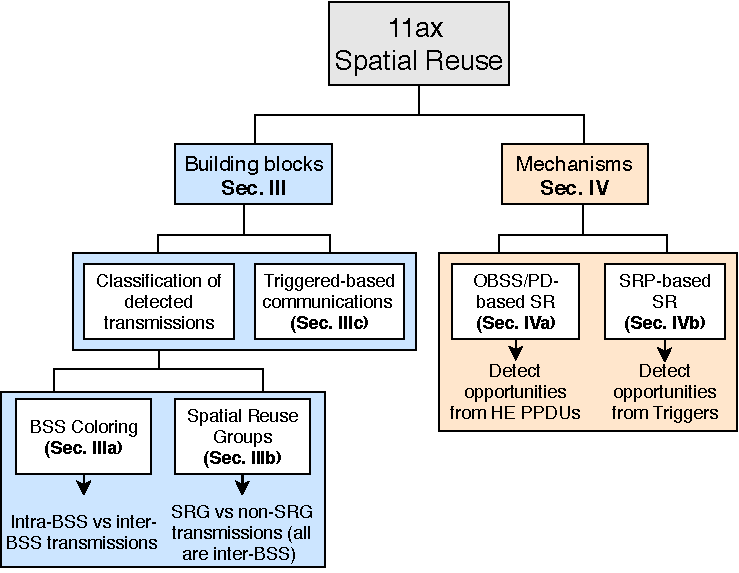
\includegraphics[width=.55\columnwidth]{sr_summary}
	\caption{Summary of the 11ax SR operation.}
	\label{fig:sr_summary}
\end{figure}

\textcolor{black}{Fig.~\ref{fig:spatial_reuse_11ax} illustrates the primary purpose of applying SR in an OBSS, where both Access Points (APs) would be able to transmit simultaneously to their corresponding stations (STAs) if using the enhanced combination of CST and transmission power (bold line). Unlike typical coverage representations in wireless networks, throughout this paper, we consider the dashed circles to be the carrier sense area of a given device (instead of the interference it generates). Accordingly, the devices that fall into the carrier sense area of a given device are considered to be detected by the latter when transmitting.} Notice that our representation assumes that \textcolor{black}{any device's} transmission power is fixed and that all the BSSs use the same frequency channel, which allows focusing on the spatial interactions only. 
\begin{figure}[ht!]
	\centering
	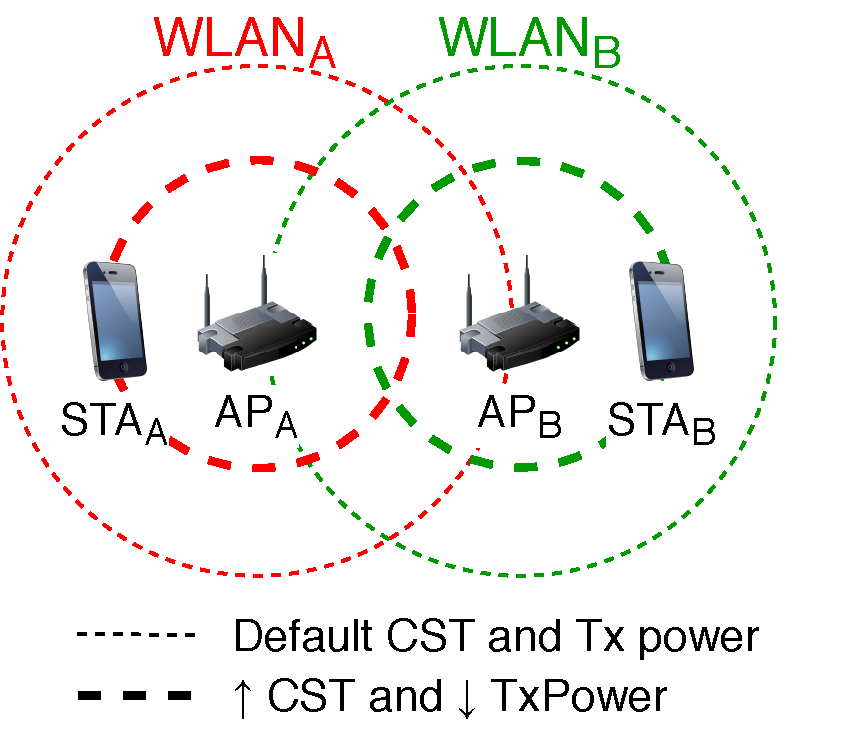
\includegraphics[width=0.38\textwidth]{fig_1.pdf}
	\caption{SR enhancement through CST adjustment and TPC. The carrier sensing area of each transmitter is graphically represented by the dashed lines.}
	\label{fig:spatial_reuse_11ax}
\end{figure}

Despite the apparent benefits of the SR operation, its actual potential is still unknown. \textcolor{black}{The fact is that SR depends on multiple factors, such as the network topology, the type of propagation effects, or the type of radio used by devices \cite{guo2003spatial, zhu2004adapting}. Moreover, sensitivity adjustment and power control may result in asymmetric links that can potentially lead to unfairness situations \cite{mhatre2007interference}.} In some cases, dynamic sensitivity and transmission power adjustment have been shown to significantly increase the network performance and contribute to reducing the effects of the well-known hidden and exposed terminal problems \cite{zhou2005balancing}. However, in some other cases, these problems may be exacerbated \cite{wilhelmi2019potential}. Modifying either the CST or the transmit power can worsen the hidden/exposed terminal problems by generating flow starvation and asymmetries.

Fig.~\ref{fig:policies_sr} shows \textcolor{black}{intuitively} the effect of increasing and decreasing both the transmission power and the sensitivity in WLANs. For instance, increasing the sensitivity may contribute to accessing the channel more often since the listening area is reduced. However, this can lead to observing a higher number of collisions by hidden nodes. Moreover, using a more aggressive channel access policy may expose the receivers to a higher level of interference, thus requiring a more robust Modulation and Coding Scheme (MCS).
\begin{figure}[ht!]
	\centering
	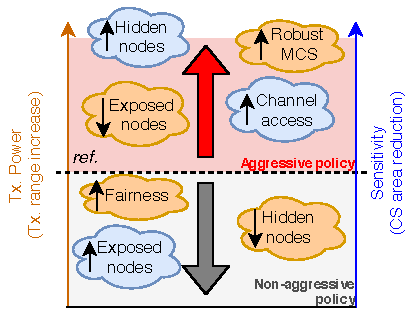
\includegraphics[width=0.4\columnwidth]{policies_sr}
	\caption{Effects of different policies concerning sensitivity adjustment and transmission power control.}
	\label{fig:policies_sr}
\end{figure}

As discussed, dealing with the spatial dimension has different implications and leads to complex inter-BSS interactions that are hard to predict beforehand. The 11ax SR operation is indeed one of the least studied features \textcolor{black}{for} next-generation WLANs, and only a few works have devised its potential. Firstly, the authors of \cite{mori2014performance} evaluated the benefits of using dynamic sensitivity thresholds for inter-BSS transmissions, given a fixed transmit power. Secondly, the work in \cite{qu2018survey} exhaustively surveyed the 11ax amendment, thus providing an overview of the first drafted SR operation. Moreover, it provided some results \textcolor{black}{of} applying SR in both indoor and outdoor scenarios, showing a higher potential for indoor deployments. Similarly, the authors of \cite{shen2018research} introduced \textcolor{black}{the SR operation as described in the 11ax amendment}. Besides, they provided a performance evaluation based on the adjustment of the inter-BSS sensitivity threshold. Their results showed significant gains when applying SR, especially for dense scenarios. 

% Contributions
Unlike in \cite{mori2014performance, qu2018survey, shen2018research}, in this paper, \textcolor{black}{we delve into the SR operation in more detail since we consider the two mechanisms included in the 11ax amendment}. In addition, our analysis of the 11ax SR is not limited to the technical information included in the amendment. Instead, we accompany our descriptions with illustrative use cases, bringing a new perspective that allows devising the real utility behind the operation. \textcolor{black}{Thus, we} go beyond the definition of the specification, shedding light on its purpose, benefits, and challenges. Our aim in this paper is to provide a comprehensive tool for researchers interested in the topic and to analyze the potential of the SR operation in future WLANs. Besides, we focus on the potential gaps in the standard to be filled by the research community. \textcolor{black}{This paper's main contributions} lie in the description, analysis, and evaluation of the 11ax SR operation. In particular:
\begin{enumerate}
	\item We provide a gentle, exhaustive, and comprehensive overview of the SR operation included in the 11ax amendment.
	\item We analytically model the 11ax SR operation for the sake of \textcolor{black}{capturing and understanding the new kinds of inter-BSS interactions that result from it}. The results of this model are verified with the Komondor 11ax-based simulator \cite{barrachina2019komondor}.
	\item We study the potential performance gains of the 11ax SR operation through simulations. 
	\item We delve into the gaps and gray areas existing in the current 11ax SR operation and \textcolor{black}{devise} future research directions in the field.
\end{enumerate}

% Document structure
The remainder of this document is structured as follows. Section \ref{section:previous_work_sr} surveys the related work on SR in WLANs. Section \ref{section:enablers_sr_11ax} describes the specifications and procedures \textcolor{black}{that} enable 11ax SR, whereas Section \ref{section:operation_sr_11ax} details the operation itself. Section~\ref{section:analytical_model} presents an analysis-based study of 11ax SR in simple scenarios. \textcolor{black}{The analysis is extended in Section~\ref{section:performance_evaluation} through the simulation of dense deployments}. Section \ref{section:ways_forwad} identifies the gaps and research opportunities found within the 11ax SR operation and explores potential ways forward. Finally, Section~\ref{section:conclusions} provides some concluding remarks.

% ----------------------------------
% -
% 	-- Previous Work on SR --
% -
% ----------------------------------
\section{Spatial Reuse techniques in IEEE 802.11 WLANs}%\section{Related Work on Spatial Reuse in IEEE 802.11 WLANs}
\label{section:previous_work_sr}

The problem of dynamic sensitivity and transmission power adjustment has been previously addressed in multiple ways. \textcolor{black}{Firstly}, we find centralized solutions such as the ones proposed in \cite{li2011achieving, jamil2016novel, nakahira2014centralized}, where the SR operation is controlled and mandated from the APs. Among these, we highlight \cite{jamil2016novel}, which uses a method based on Neural Networks (NN) to compute the best combination of sensitivity and transmit power to be used by all the BSSs in a given scenario. Nonetheless, centralized approaches require coordination and extra overhead, which is usually impractical.

\textcolor{black}{Secondly}, SR has been addressed through a decentralized perspective in \cite{chevillat2005dynamic, tang2011improving, chau2017effective, wilhelmi2019collaborative, wilhelmi2019potential}. Most of the decentralized strategies rely on collecting feedback on several performance metrics (e.g., sensed interference, packets lost). While works such as \cite{chevillat2005dynamic, tang2011improving, chau2017effective} propose adaptive mechanisms to adjust the CST and the transmission power, some others like \cite{wilhelmi2019collaborative, wilhelmi2019potential} provide probabilistic approaches based on Reinforcement Learning (RL) for finding the best possible configuration. 

Concerning IEEE 802.11ax WLANs, the Dynamic Sensitivity Control (DSC) scheme was proposed to be included in the standard, but it was never incorporated. The performance of DSC was evaluated in \cite{afaqui2015evaluation, afaqui2016dynamic, kulkarni2015taming}. Furthermore, the authors of \cite{selinis2016evaluation, selinis2017exploiting} combined DSC with BSS color schemes to devise further improvements in WLANs.

The current 11ax SR operation has nonetheless been studied to a lower extent. Based on the OBSS/PD-based SR operation, the work in \cite{selinis2018control} proposed a new mechanism to adjust the OBSS/PD threshold.\footnote{The OBSS/PD threshold refers to the sensitivity to be used for detected inter-BSS transmissions.} This mechanism, so-called Control OBSS/PD Sensitivity Threshold (COST), differs from DSC in terms of the information available in 11ax nodes. In this case, nodes need to be aware of changes in the neighboring BSSs. \textcolor{black}{Besides, \cite{ropitault2018evaluation} proposed a method for adjusting the OBSS/PD threshold in 11ax WLANs, which is based on the Received Signal Strength Indicator (RSSI).}

Unlike previous works, we focus on the IEEE 802.11ax SR operation defined in Draft v4.0 and delve into its potential through analytical modeling and a simulation tool. Moreover, we identify potential gaps and research opportunities \textcolor{black}{concerning} the amendment.

% ----------------------------------
% -
% 	-- IEEE 802.11ax Preliminaries --
% -
% ----------------------------------
\section{IEEE 802.11ax Spatial Reuse Operation: Building Blocks}
\label{section:enablers_sr_11ax}
Before delving into the 11ax SR mechanisms, we first describe the enabling concepts and features. In particular, the 11ax SR operation can be understood through \textbf{BSS coloring} and \textbf{Spatial Reuse Groups (SRG)}. In addition, we introduce the \textbf{Triggered-based (TB) transmissions} upon which the PSR operation is based.

%% BSS COLORING
\subsection{BSS coloring}	
\label{section:bss_coloring}	
BSS coloring is a key enabler of the 11ax SR operation, whereby HE nodes can rapidly identify the source of a given \textcolor{black}{detected} transmission. \textcolor{black}{When implementing BSS coloring,} a given device can effectively determine whether the channel is occupied by another device belonging to the same BSS (intra-BSS transmission, same color) or from a different one (inter-BSS transmission, different color). \textcolor{black}{The BSS color is determined by the AP (an integer between 1 and 63) and is included in the preambles of Wi-Fi frames.}\footnote{The \texttt{BSS color} field is included in the Physical Layer Convergence Procedure (PLCP) header. See Appendix \ref{section:frames} for further details.} It remains static until the AP considers to change it\textcolor{black}{, which can be provoked when a BSS color overlap is noticed (i.e., two different BSSs use the same color).} The method for selecting a new color is out of the scope of the 11ax amendment, but the advertising procedure is defined. An HE AP may announce a new BSS color via the \texttt{BSS Color Change Announcement} element, carried in Beacon, Probe Response, and (Re)Association Response frames. 

% Intra-BSS and Inter-BSS frames
\subsubsection{BSS color-based channel access rules}
\label{section:bss_color_channel_access}
When detecting a transmission, an HE node can distinguish between intra and inter-BSS frames by rapidly inspecting the \texttt{BSS color} field that is carried in every HE PLCP Protocol Data Unit (PPDU).\footnote{If the \texttt{BSS color} is not announced, frames can be classified according to the \texttt{GROUP\_ID} and \texttt{PARTIAL\_AID} in VHT PPDUs, or the MAC address in the MAC header of legacy frames (i.e., predecessor amendments of the IEEE 802.11ac).} \textcolor{black}{In practice, once a frame is detected (the received power is above the receiver's sensitivity), a device locks onto it and starts decoding the fields of the different headers. If the preamble and PHY headers can be successfully decoded, the frame is forwarded to the MAC layer for further processing (e.g., determining the transmission destination, or setting virtual carrier sensing). Otherwise, the packet is considered as interference. The accumulated interference is used to determine the state of the channel; if the accumulative interference is above the Clear Channel Assessment / Carrier Sense threshold (CCA/CS), then the channel is marked as busy. In particular, HE nodes applying SR use the default CCA/CA threshold (i.e., -82 dBm) upon detecting intra-BSS frames. On the contrary, when inter-BSS frames are detected, more aggressive PD thresholds can be applied to increase the number of parallel transmissions. Those PD thresholds are termed \textbf{non-SRG OBSS/PD} and \textbf{SRG OBSS/PD}. The SRG OBSS/PD is used when spatial reuse groups are allowed, which is discussed in detail in Section \ref{section:srg}.}

To illustrate how BSS coloring can help at enhancing SR, let us consider the scenario shown in Fig.~\ref{fig:11ax_bss_coloring_a}. We consider that $\text{AP}_\text{A}$ is prone to suffer from flow starvation if it uses the default CCA/CS value, \textcolor{black}{since it is} in the range of both $\text{AP}_\text{B}$ and $\text{AP}_\text{C}$. Note that simultaneous downlink transmissions can be held in both $\text{BSS}_\text{B}$ and $\text{BSS}_\text{C}$ because the transmitters are not in the range of each other. \textcolor{black}{The flow-in-the-middle starvation generated to $\text{BSS}_\text{A}$ can be overcome by applying an OBSS/PD threshold higher than the CCA/CS for inter-BSS frames. The way $\text{BSS}_\text{A}$ can ignore inter-BSS transmissions is illustrated in Fig.~\ref{fig:11ax_bss_coloring_b}, where $\text{AP}_\text{A}$ first identifies the source of a detected transmission by inspecting its headers (notice that the frame reception procedure has been simplified for the sake of illustration).} Then, after detecting the source of the ongoing transmissions (indicated by the color), the non-SRG OBSS/PD threshold is applied. If the OBSS/PD threshold is high enough to ignore inter-BSS transmissions, $\text{AP}_\text{A}$ can reset the PHY and continue the backoff procedure. \textcolor{black}{Besides, it is important to remark the importance of the capture effect for preventing losses from frame collisions \cite{lee2007experimental}. A widely adopted assumption to characterize IEEE 802.11 WLANs is that the Signal-to-Noise-plus-Interference Ratio (SINR) of a receiver device is sufficiently high to overcome interfering devices \cite{durvy2007modeling}.}

\begin{figure}[ht!]
	\centering
	\subfigure[Scenario]{\label{fig:11ax_bss_coloring_a}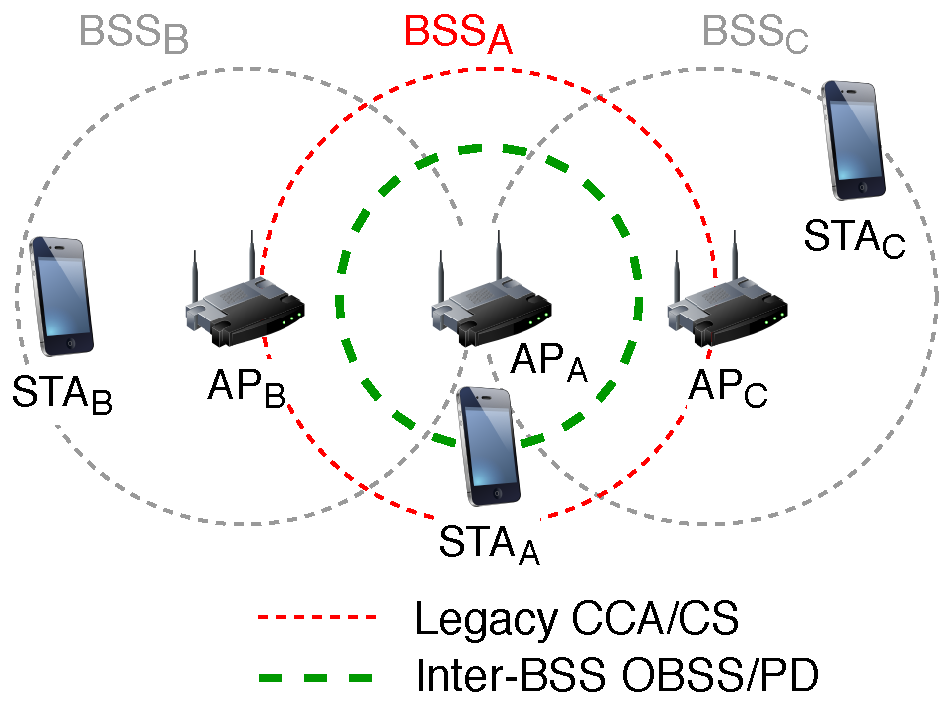
\includegraphics[width=0.35\columnwidth]{fig_2a}}
	\hspace{1cm}
	\subfigure[Packets exchange]{\label{fig:11ax_bss_coloring_b}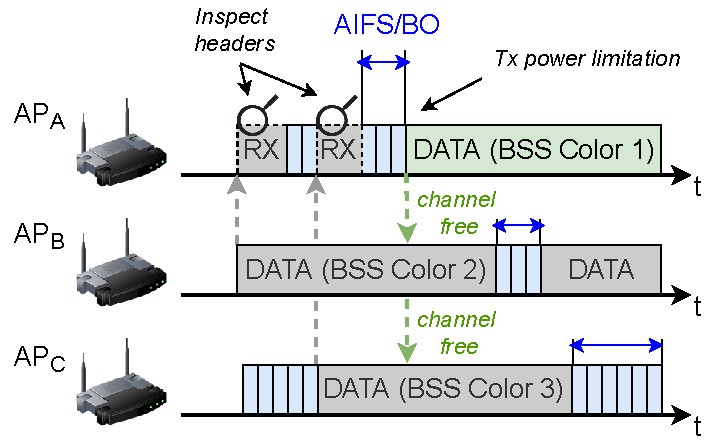
\includegraphics[width=0.45\columnwidth]{fig_4b}}
	\caption{Channel access rules based on BSS coloring. In (b), the propagation delay is considered to be negligible.}
\end{figure}

% Two NAVs
\begin{figure*}[ht!]
	\centering
	\subfigure[Scenario]{\label{fig:fig_5_a}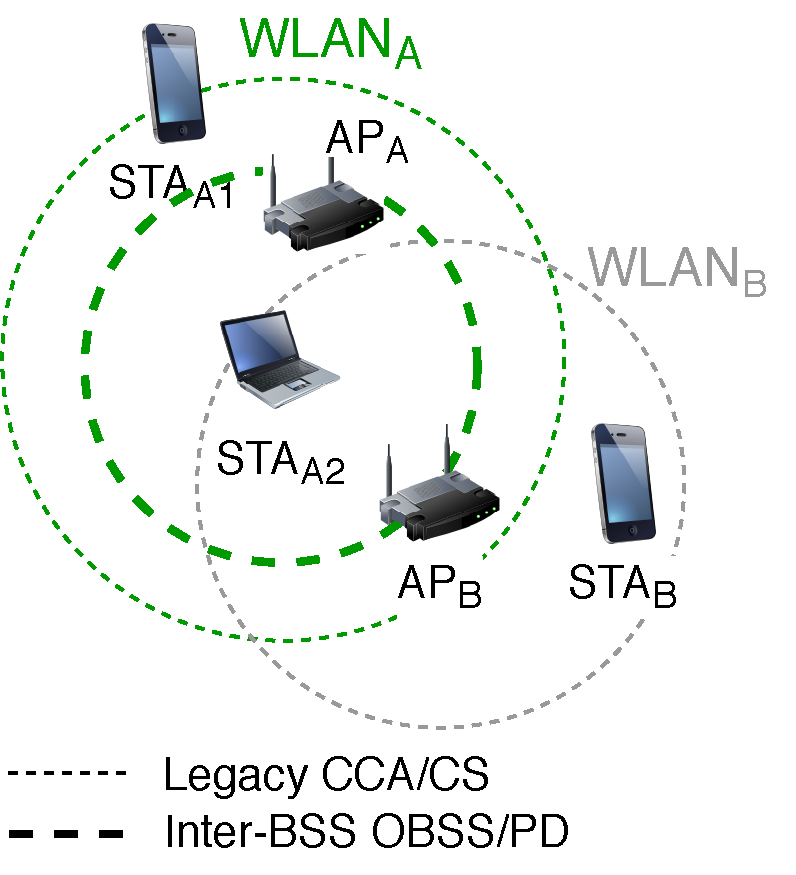
\includegraphics[width=0.35\columnwidth]{fig_5_a}}
	\hspace{1cm}
	\subfigure[Packets exchange]{\label{fig:fig_5_b}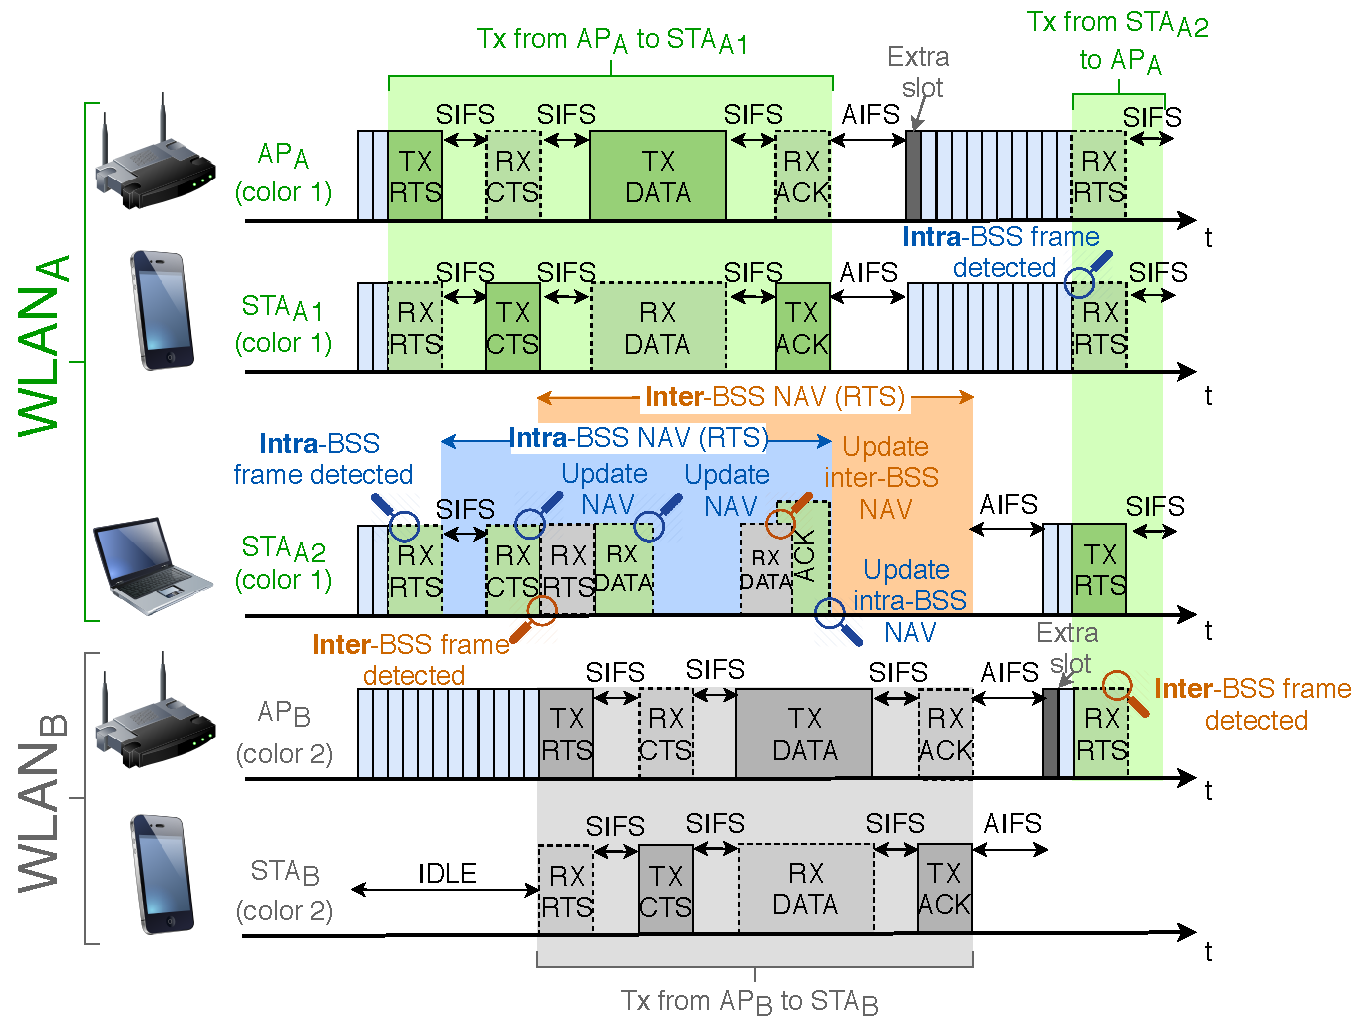
\includegraphics[width=.5\columnwidth]{fig_5_b}}
	\caption{Two NAVs operation in an OBSS.}
	\label{fig:two_navs}
\end{figure*}
\subsubsection{Two NAVs}
\label{section:two_navs}
The SR operation provides significant changes in the virtual carrier sensing procedure since two different Network Allocation Vectors (NAVs), i.e., \emph{intra-BSS NAV} and \emph{inter-BSS NAV}, have to be maintained for intra and inter-BSS frames, respectively. Accordingly, a given transmitter can decrease its backoff counter only if both NAV timers are set to zero. Otherwise, it must remain idle for at least the duration of the ongoing transmission(s),\footnote{The duration used for setting the NAV is indicated in the Duration field of RTS/CTS frames or Physical layer Service Data Units (PSDU).} which had previously activated the virtual carrier sensing. 

\textcolor{black}{The utility behind maintaining two NAVs becomes evident for dense deployments. On the one hand, the intra-BSS NAV allows protecting STAs from intra-BSS transmissions, thus reducing the effect of certain anomalies such as the hidden terminal problem. On the other hand, as a novelty, the inter-BSS NAV allows mitigating OBSS interference, which contributes to increasing the number of parallel transmissions. To illustrate the utilization of two NAVs within the SR operation, we consider the scenario shown in Fig.~\ref{fig:fig_5_a}, where packets are exchanged as illustrated in Fig.~\ref{fig:fig_5_b}.} In this scenario, $\text{BSS}_\text{A}$ and $\text{BSS}_\text{B}$ are within the same carrier sense area, provided that they both use the same CCA/CS value. In opposite, both BSSs can ignore each others' transmissions in case of using a higher OBSS/PD threshold.

Following the Distributed Coordination Function (DCF) operation, $\text{AP}_\text{A}$ initiates a downlink transmission to $\text{STA}_\text{A1}$ by first sending a Request-to-Send (RTS) frame. $\text{STA}_\text{A2}$ decodes the RTS frame and \textcolor{black}{marks it as an intra-BSS transmission} (the BSS color field matches with its color). \textcolor{black}{As a result, $\text{STA}_\text{A2}$ applies the default CCA/CS threshold to determine whether the channel remains idle or not. In this case, the sensed power is above the threshold, which makes $\text{STA}_\text{A2}$ to apply virtual carrier sensing. It is also worth mentioning that the NAV timer is confirmed in $\text{STA}_\text{A2}$ when $\text{STA}_\text{A1}$ sends the Clear-to-Send (CTS) frame to $\text{AP}_\text{A}$, because they are in range. In parallel to the abovementioned intra-BSS interactions, $\text{AP}_\text{B}$ starts a downlink transmission to $\text{STA}_\text{B}$. This transmission is detected by $\text{STA}_\text{A2}$, who shall activate the inter-BSS NAV. in this case, the frames sent by either $\text{AP}_\text{B}$ or $\text{STA}_\text{B}$ can be ignored by $\text{STA}_\text{A2}$ because the power detected is below the OBSS/PD threshold. Accordingly, $\text{STA}_\text{A2}$ can perform an uplink transmission as soon as the intra-BSS NAV is over. In this example, maintaining two NAVs allows increasing the medium re-utilization because part of the detected transmissions can be ignored.}

%%% SR groups
\subsection{Spatial Reuse Groups}
\label{section:srg}
To further enhance network efficiency, the 11ax amendment provides a mechanism for differentiating between two types of inter-BSS frames; that is to say, belonging or not to the same SRG. These groups can be formed by BSSs to achieve a more sophisticated SR operation. For instance, more aggressive channel access policies can be used for transmissions within the same SRG, \textcolor{black}{in case that the nodes of the same SRG could support higher levels of interference}. \textcolor{black}{Alternatively}, it could be the other way around. A conservative policy can be employed for the sake of minimizing collisions by hidden nodes. \textcolor{black}{Although the formation of SRGs is out of the amendment's scope,} differentiating between two OBSS/PD thresholds can be useful for capturing more subtle inter-BSS interactions. Note, as well, that SRGs could be formed online to address some issues detected by an entity controlling a set of APs (e.g., belonging to the same operator).

\textcolor{black}{For supporting SRGs,} the involved HE nodes must have indicated support for it. \textcolor{black}{HE STAs enable the SRG feature} upon the reception of an activating \texttt{Spatial Reuse Parameter Set} element (further described in Appendix \ref{section:srps}) from their AP. Then, for the following detected PPDUs, both HE APs and STAs may differentiate between SRG and non-SRG PPDUs. Note that 11ax devices can also identify the source of non-HE transmissions. Therefore, not only HE devices are supported but also legacy devices. The way of classifying SRG frames is backward compatible with previous IEEE 802.11 amendments. Technically speaking, SRG identification is made as follows:
\begin{itemize}
	\item For HE PPDUs, an HE STA inspects the \texttt{BSS color} and checks if it belongs to the same SRG. This information is kept on the \texttt{SRG BSS Color Bitmap} of the \texttt{Spatial Reuse Parameter Set}, which stores the different BSS colors that belong to the same SRG. The AP of a given BSS is responsible for maintaining the SRG BSS Color Bitmap up to date, and to inform STAs in case of noticing any change.
	\item For VHT PPDUs, same SRG is indicated if the \texttt{GROUP\_ID} parameter (included in the \texttt{RXVECTOR}\footnote{The RXVECTOR constitutes a set of parameters that the PHY layer delivers to the MAC on receiving a PPDU.}) has a value of 0, and the bit in the \texttt{SRG Partial BSSID Bitmap} field corresponding to the numerical value of \texttt{PARTIAL\_AID}\footnote{The \texttt{PARTIAL\_AID} is an identifier which, similarly to the BSS color, is used by IEEE 802.11ac WLANs to identify the source of a given transmission quickly.} (also included in the \texttt{RXVECTOR}) is set to 1. 
	\item Finally, regarding other types of PPDUs, they are classified as SRG PPDUs if the BSSID information from a MAC Protocol Data Unit (MPDU) of the PPDU is correctly received and the bit in the \texttt{SRG Partial BSSID Bitmap} field corresponding to the numerical value of BSSID is 1.
\end{itemize}

\textcolor{black}{Fig.~\ref{fig:fig_6} showcases the utility of SRG in a deployment at which using the OBSS/PD threshold homogeneously allows increasing parallel transmissions but leads to packet losses.} In particular, $\text{STA}_\text{C}$ cannot properly decode the information sent by $\text{AP}_\text{C}$ when $\text{AP}_\text{A}$ \textcolor{black}{is transmitting}. To solve this, $\text{BSS}_\text{A}$ and $\text{BSS}_\text{C}$ can form a group and employ a more conservative SRG OBSS/PD threshold to avoid simultaneous transmissions between the two BSSs. Notice that the non-SRG OBSS/PD threshold (which is more aggressive) can be still employed for transmissions held by any pair of BSSs involving $\text{BSS}_\text{B}$, thus increasing network efficiency. %5As shown, not only the formation of SRGs is a complex task, but also the definition of both non-SRG and SRG OBSS/PD thresholds.

\begin{figure}[ht!]
	\centering
	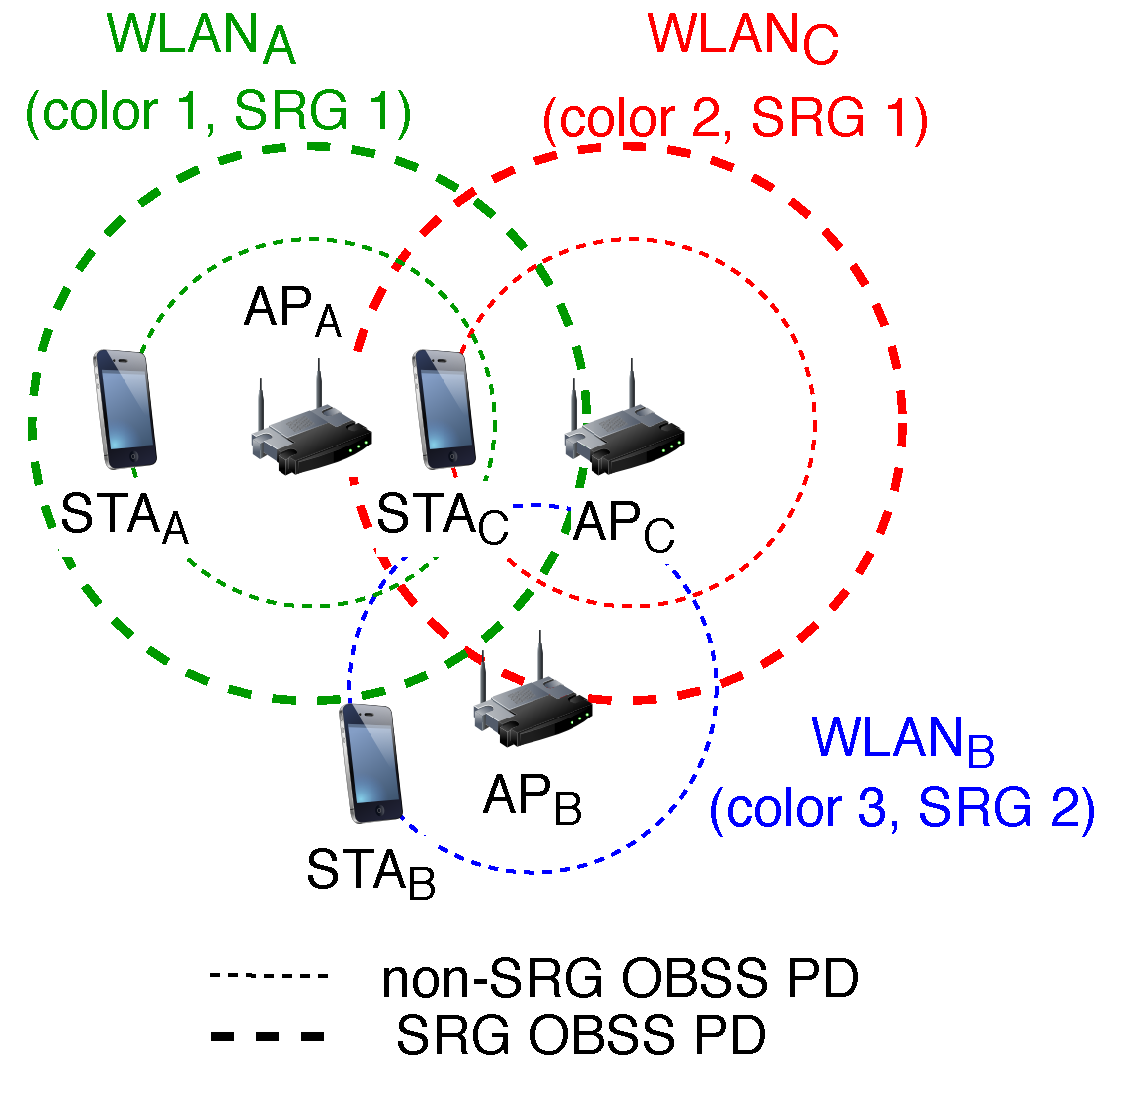
\includegraphics[width=0.4\columnwidth]{fig_6}
	\caption{Spatial Reuse Groups in an OBSS.}
	\label{fig:fig_6}
\end{figure}

% SRG and non-SRG frames
\subsubsection{SRG-based Channel Access Rules}
\label{section:srg_channel_access}
Differentiating between SRGs may provide further SR enhancements than considering only one type of inter-BSS frame. \textcolor{black}{Although the specific utilization of SRGs is also out of the 11ax amendment scope}, we devise several situations where its application can be useful. As previously pointed out, one possibility is to establish groups for BSSs whose transmissions need to be protected. In other words, an HE STA detecting an SRG frame can implement a more conservative channel access policy. Conversely, a more aggressive policy can be applied for non-SRG PPDUs, thus increasing the number of parallel transmissions. 

\textcolor{black}{To illustrate the SRG-based channel access rules, let us retake the scenario shown in Fig.~\ref{fig:fig_6}. Fig.~\ref{fig:srg_channel_access} shows the behavior of HE nodes when detecting transmissions from different SRGs. In particular, transmissions from $\text{BSS}_\text{C}$ (in blue) provoke that $\text{AP}_\text{A}$ senses the channel busy as a result of the SRG OBSS/PD-threshold. In contrast, frames detected from $\text{BSS}_\text{B}$ (in red) can be ignored by $\text{AP}_\text{A}$ because a less restrictive non-SRG OBSS/PD threshold is used. In this example, simultaneous transmissions between $\text{BSS}_\text{A}$ and $\text{BSS}_\text{B}$ are completely feasible, but the opposite occurs for $\text{BSS}_\text{A}$-$\text{BSS}_\text{C}$ interactions. Note that collisions may occur at STA$_\text{C}$ if $\text{AP}_\text{A}$ and $\text{AP}_\text{C}$ transmit simultaneously.}
%While $\text{BSS}_\text{A}$ and $\text{BSS}_\text{C}$ belong to SRG 1, $\text{BSS}_\text{B}$ belongs to SRG 2. \textcolor{blue}{Accordingly, nodes in $\text{BSS}_\text{A}$ use different OBSS/PD thresholds for inter-BSS transmissions belonging to groups 1 or 2.} 
\begin{figure}[ht!]
	\centering
	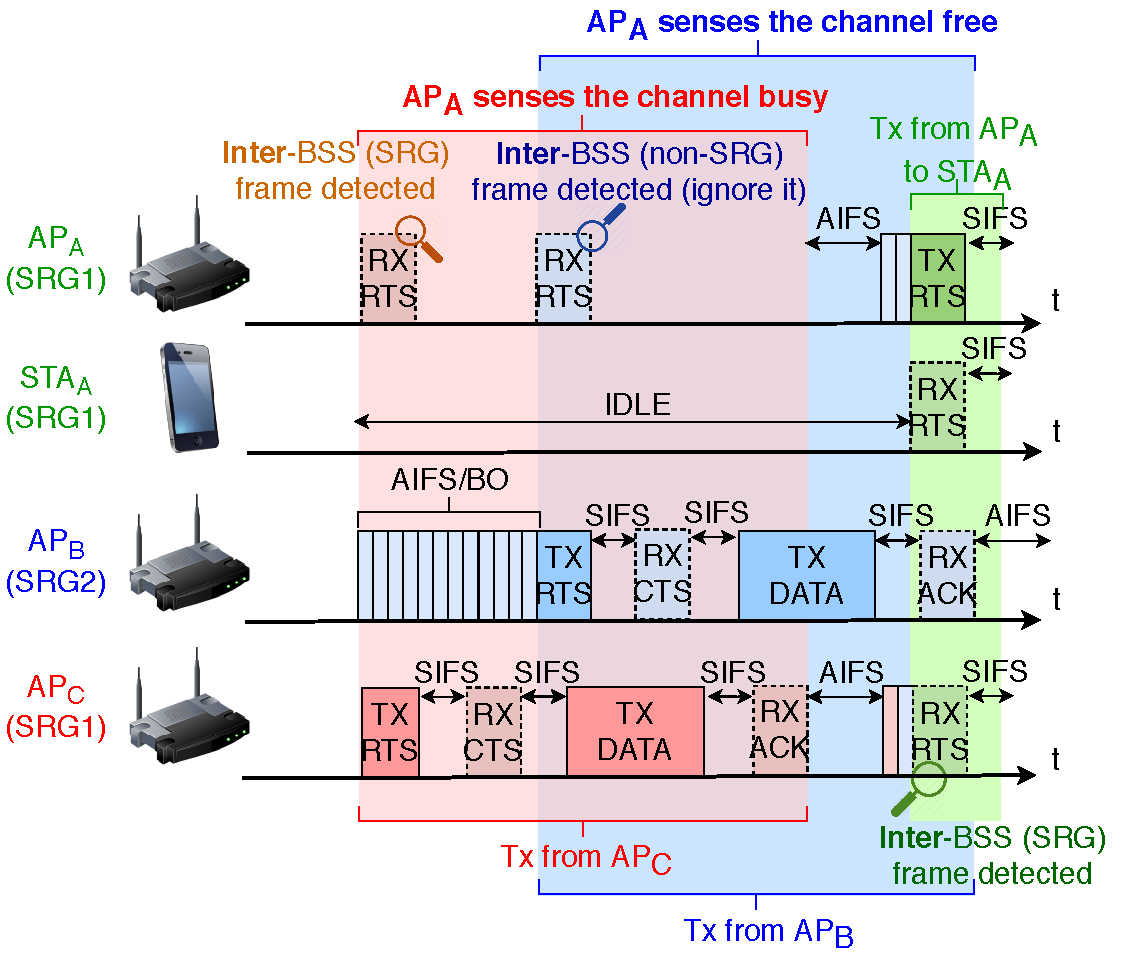
\includegraphics[width=.5\columnwidth]{fig_7}
	\caption{Packets exchange based on SRG channel access rules.}
	\label{fig:srg_channel_access}
\end{figure} 

%% TB communications
\subsection{Triggered-based communications}
\label{section:tb_communication}
\textcolor{black}{One of the 11ax SR mechanisms (i.e., PSR)} relies on TB transmissions \cite{bellalta2019ap}. Roughly, in a TB communication, an AP schedules UL transmissions from one or more STAs. To that purpose, a Trigger Frame (TF) is sent by a given AP to indicate the group of users that are allowed to transmit during the current Transmission Opportunity (TXOP), along with other relevant information. \textcolor{black}{Fig.~\ref{fig:TB_transmission_example} illustrates an example of a TB transmission. Upon successful reception of the TF sent by the AP, STAs start simultaneous TB UL transmissions,} which can be enabled by using multiple antenna technologies (i.e., MU-MIMO) or different OFDMA subcarriers. Once all the UL transmissions finish, the AP acknowledges all the packets with a multi-station block \textcolor{black}{acknowledgment} (MACK).

\begin{figure}[ht!]
	\centering
	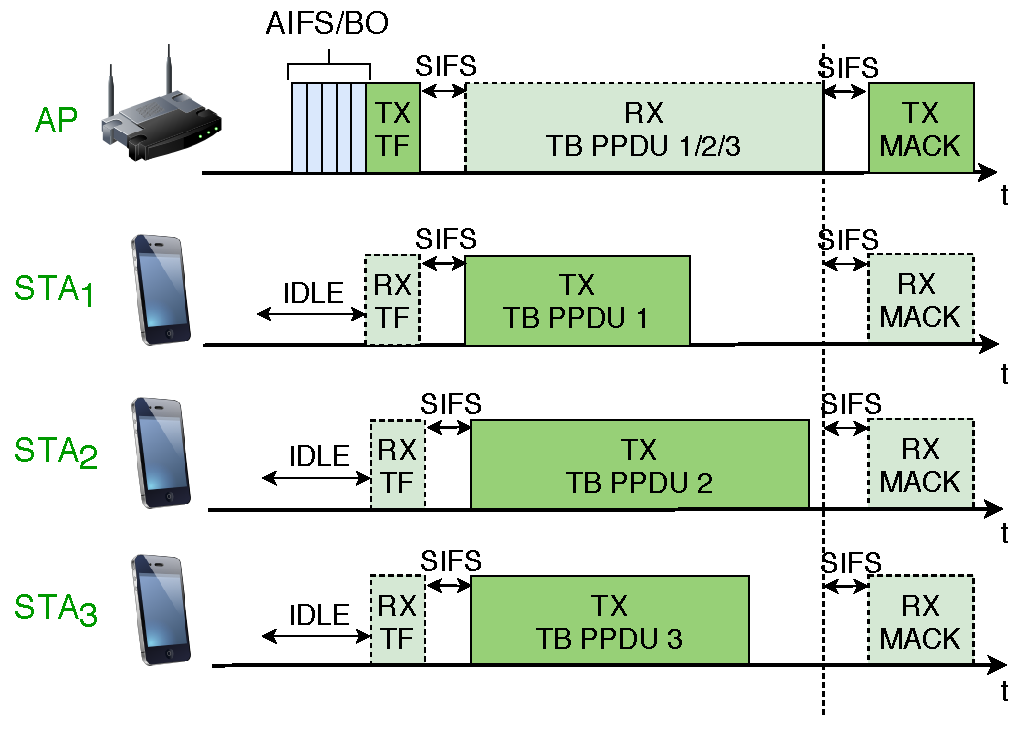
\includegraphics[width=.5\columnwidth]{fig_8}
	\caption{TB UL transmission held in a BSS.}
	\label{fig:TB_transmission_example}
\end{figure}

\textcolor{black}{The PSR operation} takes advantage of TB communications for detecting the so-called PSR opportunities. By inspecting an inter-BSS TF packet, an HE STA implementing PSR can determine the maximum allowed interference supported by the inter-BSS AP scheduling the transmission. As a result, it can transmit during the TXOP at a regulated transmission power. Further details on PSR are provided in Section \ref{section:srp_based}. Finally, it is worth mentioning that, before scheduling a UL transmission, APs can cancel the virtual carrier sensing of their STAs by sending a Contention Free End (CF-End) control frame. This is done to reduce the idle periods provoked by inter-BSS transmissions, thus enhancing network efficiency. 

% ----------------------------------
% -
% 	-- IEEE 802.11ax --
% -
% ----------------------------------

\section{IEEE 802.11ax Spatial Reuse Operation}
\label{section:operation_sr_11ax}
The IEEE 802.11ax SR operation is divided into two different mechanisms: \emph{i)} \textbf{OBSS/PD-based SR} and \emph{ii)} \textbf{PSR}. So far, we have described the elements that enable both operations, thus providing insights on the potential of applying SR. In this Section, we show the technical details of IEEE 802.11ax SR, thus embodying the concepts that have been previously introduced in Section \ref{section:enablers_sr_11ax}.

%% OBSS_PD-BASED SR
\subsection{OBSS/PD-based Spatial Reuse}
\label{section:obss_pd_based}
The OBSS/PD-based SR operation is based on CST and transmit power adjustment for detected inter-BSS frames. By knowing the source of an ongoing transmission, an HE STA may employ higher CST values \textcolor{black}{to improve} the probability of accessing the channel. In particular, upon PPDU reception, the MAC layer of a given device receives a notification from the PHY. At that moment, the node inspects the packet, and, among several operations, it determines whether the PPDU is an intra-BSS or an inter-BSS frame. The latter may be subdivided into SRG or non-SRG frames, provided that SRGs are enabled.

% General constraints
\subsubsection{General constraints}
As a general rule, the OBSS/PD threshold that is used for detected inter-BSS frames cannot exceed a certain value. This upper bound is illustrated in Fig.~\ref{fig:fig_7}, and is defined as follows:
\begin{align}\nonumber \text{OBSS/PD} \leq & \max\Big(\text{OBSS/PD}_{\min}, \min\big(\text{OBSS/PD}_{\max},\\ & \text{OBSS/PD}_{\min} + (\text{TX\_PWR}_{\text{ref}}-\text{TX\_PWR})\big)\Big), \nonumber \end{align}
where $\text{OBSS/PD}_{\min}$ and $\text{OBSS/PD}_{\max}$ are set to $-82$ dBm and $-62$ dBm, respectively, the reference power $\text{TX\_PWR}_{\text{ref}}$ is set to 21 or 25 dBm, based on the
capabilities of the device,\footnote{The $\text{TX\_PWR}_{\text{ref}}$ is set to 21 dBm at HE nodes which \texttt{Highest NSS Supported M1} field is equal or less than 1. Otherwise, the  $\text{TX\_PWR}_{\text{ref}}$ is set to 25 dBm. The \texttt{Highest NSS Supported M1} subfield is part of the \texttt{Tx Rx HE MCS Support} field of the \texttt{HE Capabilities element}.} and $\text{TX\_PWR}$ is the transmission power at the antenna connector in dBm of the HE node \textcolor{black}{identifying the SR-based TXOP}.
\begin{figure}[ht!]
	\centering
	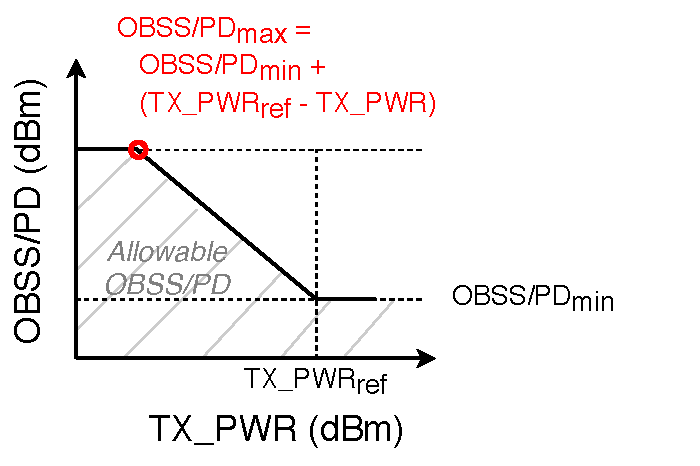
\includegraphics[width=0.4\columnwidth]{fig_10}
	\caption{Graphical representation of the adjustment rules for OBSS/PD and transmission power \cite{tgax2019draft}.}
	\label{fig:fig_7}
\end{figure}

Note that the $\text{OBSS/PD}$ threshold is defined for 20 MHz PPDUs received on the primary channel, but, in general, this value depends on the bandwidth used. In particular, the $\text{OBSS/PD}$ threshold increases 3 dB each time the channel width is doubled, as shown in Table \ref{tbl:sensitivity_channel_width}.
\begin{table}[ht!]
	\centering
	\begin{tabular}{|c|c|}
		\hline
		\textbf{Channel width} & \textbf{OBSS/PD} \\ \hline
		40 MHz & $\text{OBSS/PD}_{20 \text{MHz}}$ + 3 dB \\ \hline
		80 MHz & $\text{OBSS/PD}_{20 \text{MHz}}$ + 6 dB \\ \hline
		160 MHz or 80+80 MHz &  $\text{OBSS/PD}_{20 \text{MHz}}$ + 9 dB \\ \hline
	\end{tabular}
	\caption{Effect of the channel width on the OBSS/PD threshold.}
	\label{tbl:sensitivity_channel_width}
\end{table}

% SRG constraints
\subsubsection{SRG-based constraints}	
\textcolor{black}{Besides the general rules for the OBSS/PD, further constraints apply when considering SRGs. In particular, an AP can define certain tolerance margins (or offsets) for setting both SRG and non-SRG OBSS/PD thresholds (see Tables \ref{tbl:non-srg} and \ref{tbl:srg}). The minimum and maximum OBSS/PD offsets must verify the following conditions:}
\begin{enumerate}
	\item -82 dBm $\leq$ -82 dBm + SRG OBSS/PD Min Offset $\leq$ -62 dBm 
	\item SRG OBSS/PD Min Offset $\leq$ SRG OBSS/PD Max Offset
	\item SRG OBSS/PD Max Offset + -82 dBm $\leq$ -62 dBm 
	\item Non-SRG OBSS/PD Max Offset + -82 dBm $\leq$  -62 dBm
\end{enumerate}

\begin{table}[ht!]
	\centering
	\resizebox{.8\columnwidth}{!}{\begin{tabular}{|c|c|c|c|}
			\hline
			\begin{tabular}[c]{@{}c@{}}\textbf{OBSS/PD SR} \\\textbf{disallowed}\end{tabular} & \textbf{Non-SRG Offset} & \begin{tabular}[c]{@{}c@{}}\textbf{Non-SRG} \\\textbf{OBSS/PD Min}\end{tabular} & \begin{tabular}[c]{@{}c@{}}\textbf{Non-SRG} \\\textbf{OBSS/PD Max}\end{tabular} \\ \hline
			Unspecified & Unspecified & -82 & -62 \\ \hline
			0 & 0 & -82 & -62 \\ \hline
			0 & 1 & -82 & \begin{tabular}[c]{@{}c@{}}-82 + Non-SRG\\ OBSS/PD Max off.\end{tabular}\\ \hline
			1 & Don't care & -82 & -82 \\ \hline
	\end{tabular}}
	\caption{Minimum and maximum non-SRG OBSS/PD threshold (in dBm) to be used by a given HE STA, according to the information provided by the AP in parameters \texttt{OBSS/PD SR Disallowed} and \texttt{Non-SRG Offset Present}.}
	\label{tbl:non-srg}
\end{table}

\begin{table}[ht! ]
	\centering
	%\resizebox{\columnwidth}{!}{}
	\begin{tabular}{|c|c|c|}
		\hline
		\textbf{SRG field} & \textbf{SRG OBSS/PD Min} & \textbf{SRG OBSS/PD Max} \\ \hline	\begin{tabular}[c]{@{}c@{}}Unspecified\end{tabular} & N/A & N/A \\ \hline
		0 & N/A & N/A \\ \hline
		1 & \begin{tabular}[c]{@{}c@{}}-82 + SRG OBSS/PD\\ Min Offset\end{tabular} & \begin{tabular}[c]{@{}c@{}}-82 + SRG OBSS/PD\\ Max Offset\end{tabular} \\ \hline
	\end{tabular}
	\caption{Minimum and maximum SRG OBSS/PD values (in dBm) to be used by a given HE STA, according to the information provided by the \texttt{SRG} field. If SRG is not activated (or its value is unspecified), PPDU frames cannot be classified as SRG frames.}
	\label{tbl:srg}
\end{table}

Note, as well, that the way of computing SRG and non-SRG OBSS/PD thresholds is not defined in the standard, thus opening the door to new contributions. \textcolor{black}{In this regard, the work in \cite{tgax2016obss_pd_evaluation} proposed using the RSSI of received beacons to compute the OBSS/PD thresholds.}

% Tx Power restriction
\subsubsection{Transmit power restriction}	\label{section:tx_power_restriction}
So far, we have referred to CST adjustment, but transmit power control is also an important part of the SR operation. In particular, a power restriction is imposed for any transmission occurring as a result of a detected SR TXOP (i.e., after ignoring a given inter-BSS frame through the OBSS/PD-based SR operation). The maximum allowed transmission power ($\text{TX\_PWR}_{\max}$) is given by:
\begin{equation}
\text{TX\_PWR}_{\max} = \text{TX\_PWR}_{\text{ref}} - (\text{OBSS/PD} -\text{OBSS/PD}_{\min})
\label{eq:power_restriction}
\end{equation}

The previous equation holds for $\text{OBSS/PD}_{\max} \geq \text{OBSS/PD} > \text{OBSS/PD}_{\min}$. Otherwise, the maximum transmission power is unconstrained. By applying a power restriction, \textcolor{black}{the amendment aims to reduce the impact of concurrent transmissions taking place due to SR. Simply put, the higher the OBSS/PD threshold (more inter-BSS transmissions can be ignored), the lower the transmit power (less interference should be generated).} The transmission power restriction lasts until the end of the SR TXOP identified by an HE node, which starts when its backoff reaches zero. Notice that this period depends on the duration of the active transmission(s) used for detecting the SR TXOPs. 

\subsubsection{Example of OBSS/PD Spatial Reuse}
% EXAMPLES
To illustrate the OBSS/PD-based SR operation in detail, we propose the scenario shown in Fig.~\ref{fig:fig_8_a}, from which we focus on $\text{STA}_\text{C2}$. In this scenario, several potential interfering devices (belonging to $\text{BSS}_\text{A}$ and $\text{BSS}_\text{B}$) surround $\text{STA}_\text{C2}$. In particular, when using the default CCA/CS, all the APs are able to transmit simultaneously. However, $\text{STA}_\text{C2}$ may suffer flow starvation because of its unprivileged location.
\begin{figure}[ht!]
	\centering
	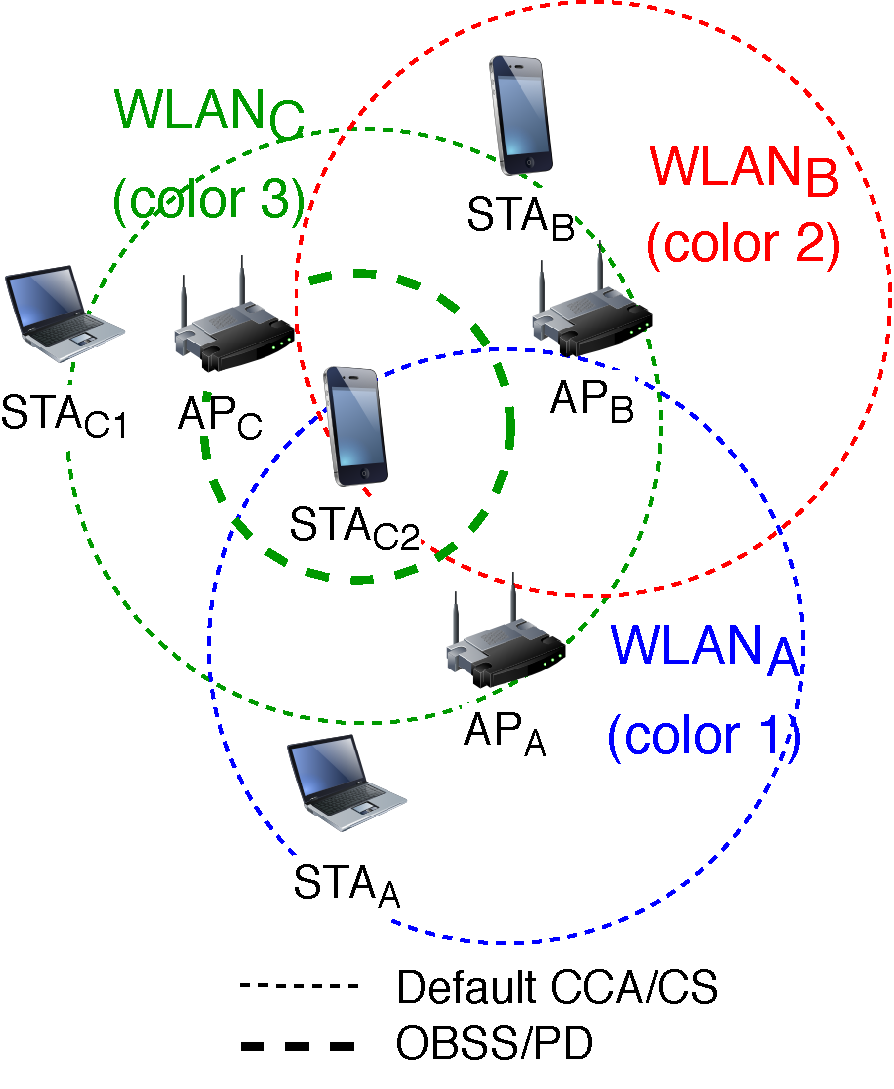
\includegraphics[width=0.35\columnwidth]{fig_11}
	\caption{Scenario for showcasing the OBSS/PD SR operation.}
	\label{fig:fig_8_a}
\end{figure}

\textcolor{black}{To overcome the high interference at which $\text{STA}_\text{C2}$ is exposed to, the OBSS/PD threshold can be applied to ignore inter-BSS transmissions. Fig.~\ref{fig:fig_12} illustrates the behavior of $\text{STA}_\text{C2}$ when applying OBSS/PD-based SR. Notice that any detected SR TXOP is subject to a power restriction (see \eqref{eq:power_restriction}), and that different power restrictions can be applied as a result of applying different OBSS/PD thresholds (of SRG and non-SRG type). That said, the following activity points (displayed in yellow) are observed from Fig.~\ref{fig:fig_12}:}
\begin{enumerate}
	\item $\text{STA}_\text{C2}$ analyzes the RTS frame sent by $\text{AP}_\text{A}$ and classifies it as an inter-BSS frame. As a result, it applies a given OBSS/PD value that allows sensing the channel idle ($\text{RSSI}_{\text{A} \rightarrow \text{C2}} < \text{OBSS/PD}$). \textcolor{black}{A first power restriction is considered by $\text{STA}_\text{C2}$.}
	\item The same procedure is followed at $\text{STA}_\text{C2}$ when detecting the RTS frame transmitted by $\text{AP}_\text{C}$. However, the transmission cannot be ignored this time because it is an intra-BSS transmission ($\text{RSSI}_{\text{C} \rightarrow \text{C2}} < \text{CCA/CS}$ ).
	\item As for points 1) and 2), $\text{AP}_\text{B}$'s transmission is ignored by $\text{STA}_\text{C2}$ because $\text{RSSI}_{\text{B} \rightarrow \text{C2}} < \text{OBSS/PD}$. Again, a new power restriction is considered.
	\item Finally, $\text{STA}_\text{C2}$ transmits by taking advantage of the detected SR TXOPs. \textcolor{black}{The transmission is nonetheless subject to the most restrictive limitation among all the collected power restrictions (PRs)}. In particular, $\text{TX PWR}_{max} = \min(\text{PR}_1, \text{PR}_2)$.\footnote{Notice that, once $\text{STA}_\text{C2}$ transmits under the power restriction, the ACK sent by $\text{STA}_\text{B}$ can be ignored, so that a new power restriction is not defined.}
\end{enumerate}

\begin{figure}[ht!]
	\centering
	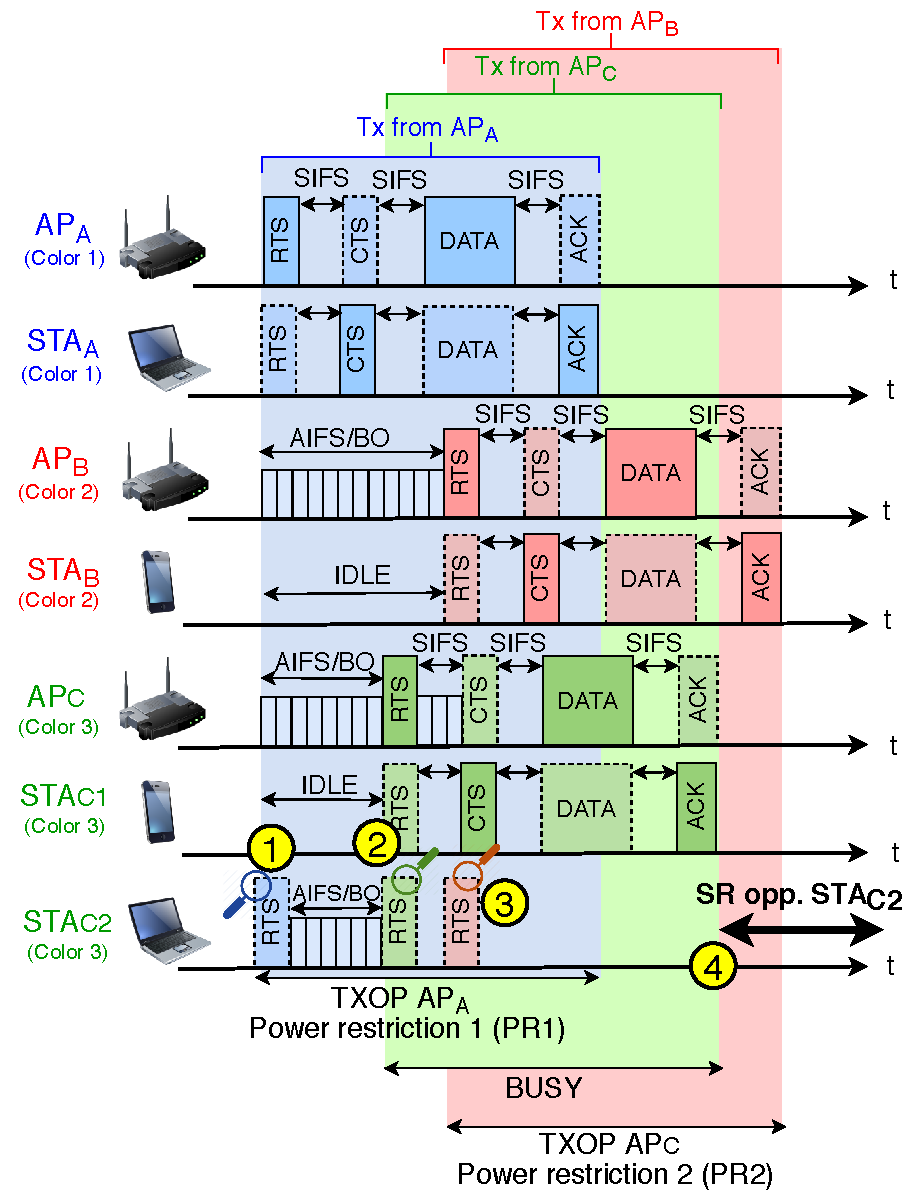
\includegraphics[width=.55\columnwidth]{fig_12}
	\caption{Example of the OBSS/PD-based SR operation. $\text{STA}_\text{C2}$ applies different OBSS/PD values according to the source of detected transmissions.}
	\label{fig:fig_12}
\end{figure}

%%% PSR
\subsection{Parametrized Spatial Reuse}
\label{section:srp_based}	
The PSR operation is based on TB transmissions and requires cooperation among the participating BSSs. On the one hand, we find nodes taking advantage of PSR opportunities (i.e., the \emph{opportunists}). These nodes identify PSR opportunities from detected TB transmissions. On the other hand, we find the \emph{transmission holders}, which perform TB transmissions and indicate support for the PSR operation \textcolor{black}{in the headers of the TF. To identify a PSR opportunity,} an opportunist must check whether the TB PPDUs that follow a given TF packet can be ignored or not. To do so, the \textcolor{black}{opportunist's intended transmission power} must not exceed the requirements imposed by the transmission holder. \text{The latter encapsulates} those requirements through the \texttt{PSR\_INPUT} parameter. This parameter is indicated in the TF and can take any of the discrete values shown in Table \ref{tbl:sr_subfield_encoding_TB_ppdu} \textcolor{black}{and is computed as:}
\begin{equation}
\text{PSR INPUT} = \text{TX PWR}_\text{AP} + \text{I}_\text{AP}^{\max},
\label{eq:srp_input}
\nonumber
\end{equation}
where $\text{TX PWR}_\text{AP}$ is the normalized transmit power in dBm at the output of the antenna connector, and $\text{I}_\text{AP}^{\max}$ is a normalized value in dB that captures the maximum allowed interference at the transmission holder.\footnote{In particular, $\text{I}_\text{AP}^{\max}$ is computed as the target RSSI indicated in the TF minus the minimum SNR granting a 10\% PER (based on the highest MCS to be used for transmitting the UL HE TB PPDU). A safety margin (set by the AP) is also included not to exceed 5 dB.}

\begin{table}[ht!]
	\centering			
		\begin{tabular}{|c|c|c|c|}
			\hline
			\textbf{Value} & \textbf{Meaning} & \textbf{Value} & \textbf{Meaning} \\ \hline
			0 & PSR\_DISALLOW & 8 & PSR = -44 dBm \\ \hline
			1 & PSR = -80 dBm & 9 & PSR = -41 dBm \\ \hline
			2 & PSR = -74 dBm & 10 & PSR = -38 dBm \\ \hline
			3 & PSR = -68 dBm & 11 & PSR = -35 dBm \\ \hline
			4 & PSR = -62 dBm & 12 & PSR = -32 dBm \\ \hline
			5 & PSR = -56 dBm & 13 & PSR = -29 dBm \\ \hline
			6 & PSR = -50 dBm & 14 & PSR $\geq$ -26 dBm \\ \hline		7 & PSR = -47 dBm & 15 & \begin{tabular}[c]{@{}c@{}}PSR\_AND\_NON-\\ SRG\_OBSS-PD\_\\ PROHIBITED\end{tabular} \\ \hline
	\end{tabular}
	\caption{PSR subfield encoding for Trigger and HE TB PPDU frames \cite{tgax2019draft}.}
	\label{tbl:sr_subfield_encoding_TB_ppdu}
\end{table}

Once an opportunist inspects the PSR value of the detected TF\footnote{The PSR can be extracted either from the \texttt{SPATIAL REUSE} field, which is included in the \texttt{Common Info} field of the Trigger frame, or the \texttt{SIG-A PSR} field of the HE TB PPDU.} and confirms that the intended transmission power is acceptable, it transmits during the duration of the TB PPDU(s) (indicated in the \texttt{Common Info} field). In particular, the intended transmission power must be below the value of PSR minus the Received Power Level (RPL), which is measured from the legacy portion of the TF (i.e., from PHY headers).

\begin{figure}[ht!]
	\centering
	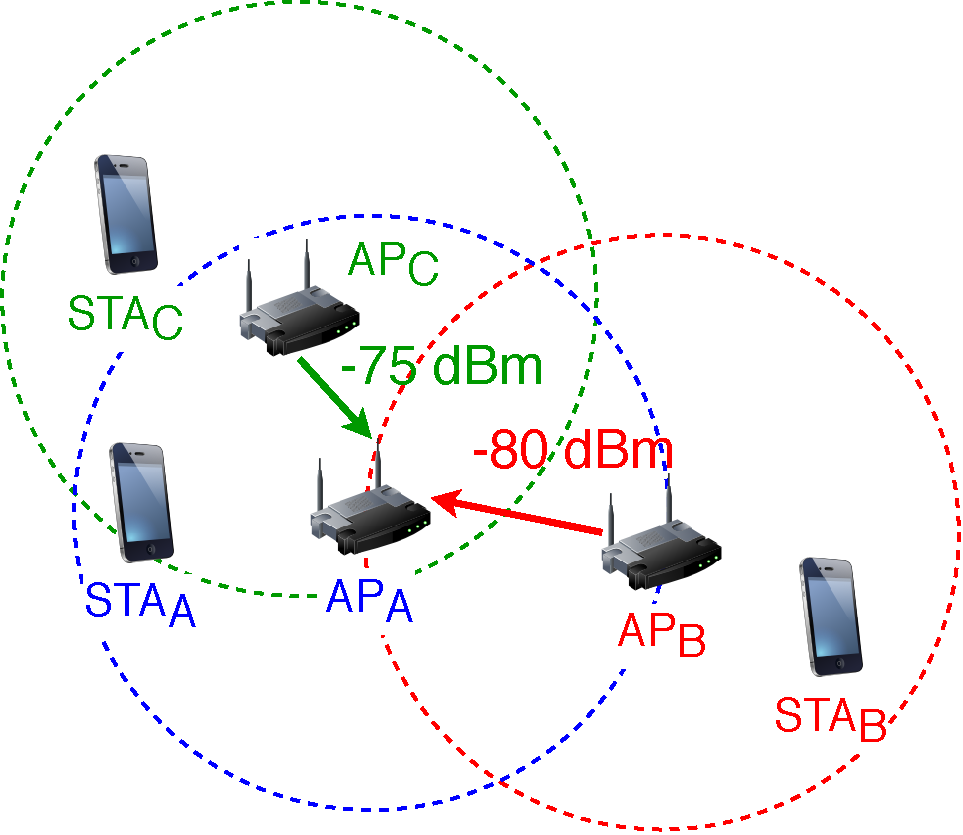
\includegraphics[width=0.35\columnwidth]{fig_13a}
	\caption{Scenario for showcasing the PSR operation.}
	\label{fig:fig_13a}
\end{figure}

\begin{figure}[ht!]
	\centering
	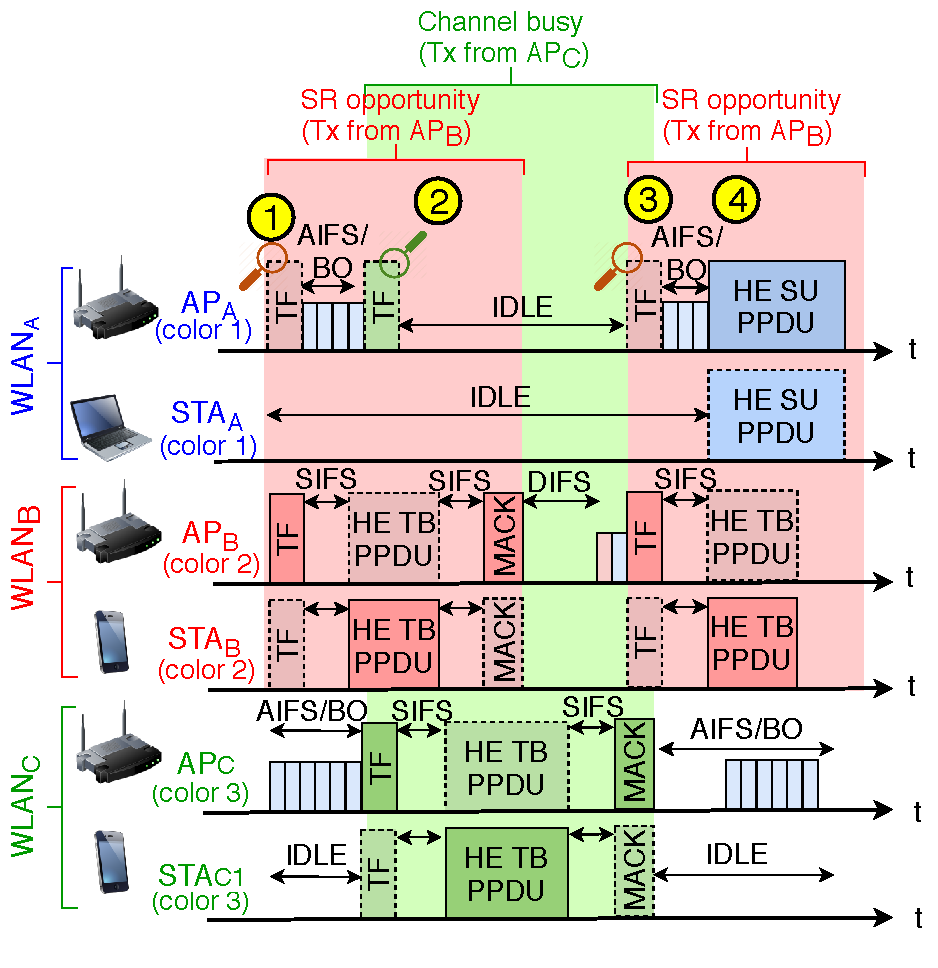
\includegraphics[width=.55\columnwidth]{fig_13b}
	\caption{Packets exchange according to the PSR operation.}
	\label{fig:fig_13b}
\end{figure}

\textcolor{black}{To illustrate the PSR operation, refer to the scenario in Fig.~\ref{fig:fig_13a}, where we focus on $\text{AP}_\text{A}$. According to the interference sensed by each other AP, Fig.~\ref{fig:fig_13b} shows $\text{AP}_\text{A}$'s behavior when applying PSR. In particular:}
\begin{enumerate}
	\item $\text{AP}_\text{A}$ detects a PSR TXOP from $\text{AP}_\text{B}$'s TF packet. \textcolor{black}{Since $\text{AP}_\text{A}$'s intended transmit power for the next queued packet is below the PSR indicated by $\text{AP}_\text{B}$ minus the RPL, $\text{AP}_\text{A}$'s backoff keeps counting down.}
	\item As soon as $\text{AP}_\text{C}$ transmits a TF, the PSR TXOP previously detected by $\text{AP}_\text{A}$ is canceled because the transmit power condition no longer holds. As a result, the channel becomes busy and the backoff is frozen.
	\item \textcolor{black}{A new PSR TXOP is detected  from the new $\text{AP}_\text{B}$'s transmission, even if $\text{BSS}_\text{C}$ is still transmitting.}
	\item Once $\text{BSS}_\text{C}$'s transmission is over, $\text{AP}_\text{A}$ \textcolor{black}{consumes the backoff} and transmits according to the last detected PSR TXOP.
\end{enumerate}

% ----------------------------------
% -
% 	-- Analytical Framework --
% -
% ----------------------------------
\section{Model and Simulation of the 11ax Spatial Reuse Operation}
\label{section:analytical_model}

\textcolor{black}{Evaluating the performance of} the IEEE 802.11ax SR operation is crucial to understand its implications and potential gains. However, it turns out to be a challenging task due to the complex (and still unknown) inter-BSS interactions generated by adjusting the sensitivity and the transmission power. \textcolor{black}{In this regard, analytical models contribute to understanding the behavior of Wi-Fi nodes applying SR. Although analytical models need to make assumptions to characterize MAC layer phenomena, the most common models have been shown to provide accurate predictions \cite{malone2007verification, huang2010validity}. The work in \cite{malone2007verification} verified the accuracy of several widely adopted assumptions of IEEE 802.11 MAC models through experimental testbed.}

To the best of our knowledge, none of the previous literature has attempted to model the 11ax SR operation. \textcolor{black}{Nevertheless, we find some works that analyze the impact of sensitivity adjustment and transmit power control in wireless networks. In this regard, we find SINR-based methods \cite{gupta2000capacity, guo2003spatial}, which allow characterizing radio links. However, these methods typically consider the worst-case interference (i.e., nodes are assumed to transmit permanently), which entails neglecting spectrum access coordination and losing insights on the MAC operation.}

\textcolor{black}{Apart from SINR-based methods, Stochastic Geometry (SG) has been applied for SR. SG models the random nature of dense wireless networks by defining a set of nodes (typically, based on random point processes) and deriving statistical properties from them. In telecommunications, SG has been widely applied to model the behavior of users and to estimate metrics such as the outage probability or the throughput per area \cite{elsawy2016modeling}. Concerning SR, the works in \cite{zhao2016stochastic, zhang2015stochastic, iwata2019stochastic} apply SG to model the effect of tuning the sensitivity threshold in WLANs. However, SG models focus on PHY layer effects and fail to capture the asymmetries in SR.}

\textcolor{black}{To address the limitations posed by the abovementioned models, we propose characterizing SR through Continuous Time Markov Networks (CTMNs) \cite{bellalta2014throughput, bellalta2017throughput}. The CTMN model allows capturing both the PHY and MAC layers on estimating the throughput of a CSMA/CA network.} The analytical model presented in this work aims to shed light on the effects of SR for next-generation BSSs.

Apart from the analytical model, we characterize SR in the Komondor simulator,\footnote{The implementation of SR can be found in Komondor v3.0, available in \url{https://github.com/wn-upf/Komondor/releases/tag/v3.0}.} \textcolor{black}{The DCF's implementation in Komondor has been validated against ns-3 and the CTMN and Bianchi models \cite{barrachina2019komondor}. The Komondor simulator was conceived to allow the low-complexity integration of novel mechanisms included in new IEEE 802.11 standards, and to simulate massively crowded next-generation deployments in a reasonable amount of time. In particular, the implementation of SR in Komondor is expected to showcase the effects of using SR in dense scenarios. Besides, simulating SR allows us to validate the inter-BSS interactions studied through the analytical model, and to address the assumptions done by CTMNs for representing the behavior of WiFi devices more realistically.} Notice that the 11ax SR operation has not been yet fully implemented in any other well-known simulator. At the time of publishing this article, SR is still being developed for ns-3.\footnote{It is planned to be included in the following repository: \url{https://gitlab.com/nsnam/ns-3-dev}.}

Before getting into the analysis of 11ax SR through CTMNs, it is important to mention that we have focused on the OBSS/PD-based operation described in Section \ref{section:obss_pd_based}, which has drawn much more attention than PSR. Therefore, from now onwards, we may refer to the OBSS/PD-based SR operation simply as SR. The implementation and modeling of PSR is left as future work.

\subsection{Introduction to Continuous Time Markov Networks}
\textcolor{black}{The CTMN model captures the CSMA/CA operation in IEEE 802.11 WLANs through states that represent the set of potentially overlapping BSSs that are active at a given moment. Transitions between states occur when BSSs become active (i.e., they gain access to the medium) or abandon the channel (i.e., their transmission finishes). While the arrival rate ($\lambda$) characterizes channel access, the time it takes for transmitting data is derived from the service rate ($\mu$). Based on the transition probabilities, it is straightforward to obtain every state's probability, which allows computing the long-term throughput experienced by the different BSSs.}

It is worth pointing out some assumptions made by the CTMN model. \textcolor{black}{First, downlink traffic is considered, and the interference produced in uplink transmissions (e.g., ACKs) is neglected. Second, the backoff procedure for accessing the medium is continuous in time. Thus, collisions due to backoff expiring at the same instant are not captured by the model. Despite the continuous backoff assumption, the CTMN model has been shown to characterize WLAN deployments accurately \cite{bellalta2016throughput,michaloliakos2016performance} and to be particularly useful for depicting inter-AP interactions.}

%\begin{figure}[h!!!!]	
%	\centering
%	
\includegraphics[width=0.45\columnwidth]{ctmn}
%	\caption{CTMN of $\text{BSS}_\text{A}$.} 
%	\label{fig:ctmn}
%\end{figure}

%For the sake of illustration, let us consider Fig. \ref{fig:ctmn}, which represents the CTMN of a single BSS, namely $\text{BSS}_\text{A}$. In the CTMN, $s_0$ is the empty state (the channel is idle) and $s_1$ indicates that $\text{BSS}_\text{A}$ is transmitting in a given channel. Regarding the transition rates between states, we find two different types: \emph{i)} AP activates, and \emph{ii)} AP finishes a transmission. While \emph{i)} is related to the necessary time for a given node to access the channel (characterized by the arrival rate $\lambda$), \emph{ii)} depends on the time spent by a given node for transmitting data (characterized by the service rate $\mu$). Based on the transition probabilities, one can obtain every state's probability, which allows computing the long-term throughput experienced by the different BSSs.

In this work, the 11ax SR operation has been implemented as part of the Spatial Flexible Continuous Time Markov Network (SFCTMN) framework \cite{barrachina2019dynamic, barrachina2019overlap, wilhelmi2019potential}.\footnote{A dedicated Github branch of SFCTMN has been provided for single-channel spatial reuse \cite{wilhelmi2019sfctm_spatial_reuse}.} This framework allows generating the CTMN of a given WLAN deployment, based on the spatial distribution of nodes and their configuration (e.g., range of channels used, transmission power, sensitivity...). It is important to remark that additive interference is considered, which results from the combination of different simultaneous transmissions. \textcolor{black}{This aspect is key to represent the spatially-distributed interactions that occur as a result of applying SR.}

\textcolor{black}{Concerning the 11ax SR operation, we differentiate between different types of states, which stem from the set of sensitivity levels that each BSS can apply (default CCA/CS, non-SRG OBSS/PD, and SRG OBSS/PD). Notice that sensitivity adjustment potentially leads to new interactions (e.g.,~concurrent transmissions). Moreover, the transmit power limitation, which depends on the OBSS/PD threshold, affects to the MCS used for a given transmission.}
%Moreover, traffic is considered to be saturated in all the nodes, so that pure SR-based interactions become \textcolor{blue}{apparent}.

%%% Simple OBSS/PD-based interactions
\subsection{Simple inter-BSS interactions}
\label{section:simple_interactions}
\textcolor{black}{To showcase the inter-BSS interactions that result from applying SR, we introduce \emph{Toy scenario 1} (illustrated in Fig.~\ref{fig:toy_scenario_1b}). We first consider that only $\text{BSS}_\text{A}$ implements SR. Fig.~\ref{fig:cs_toy_scenario_1a} and Fig.~\ref{fig:cs_toy_scenario_1b} illustrate the carrier sense areas based that result from using the default CCA/CS and the OBSS/PD threshold, respectively. The CTMNs capturing the inter-BSS interactions taking place in each setting are shown in Fig.~\ref{fig:ctmn_toy_scenario_1a} and Fig.~\ref{fig:ctmn_toy_scenario_1b}, respectively. Notice that the long-term probability of each state is shown in parentheses.}

\begin{figure*}[h!]
	\centering
	% Situation 1
	\subfigure[Sensing area (CCA/CA = -82 dBm)]{\label{fig:cs_toy_scenario_1a}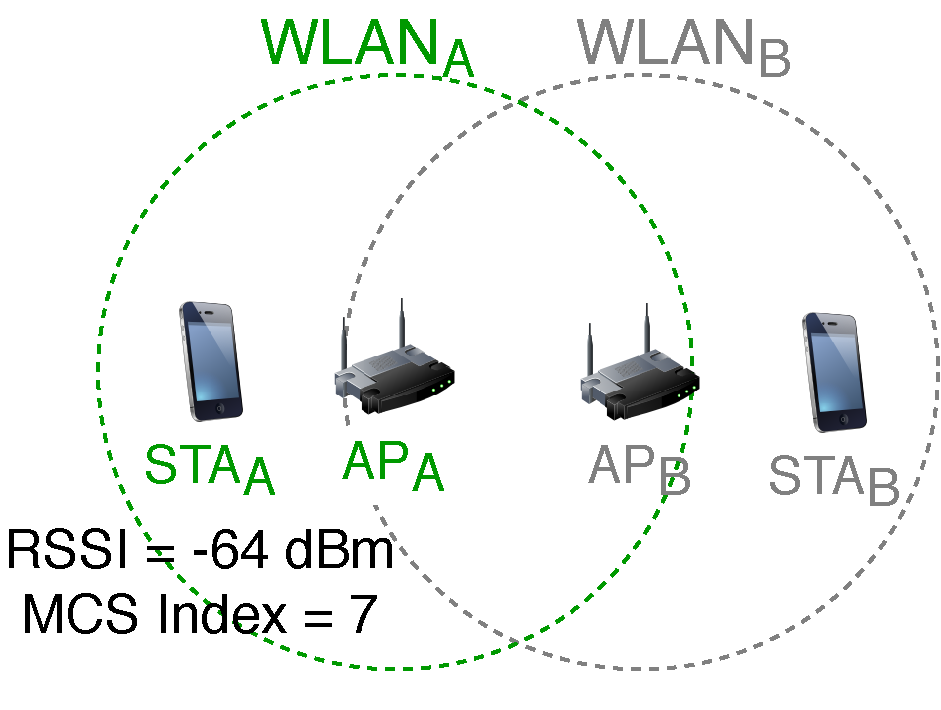
\includegraphics[width=0.4\textwidth]{fig_15a}}
	\hspace{1cm}
	% CTMN 1
	\subfigure[CTMN (CCA/CA = -82 dBm)]{\label{fig:ctmn_toy_scenario_1a}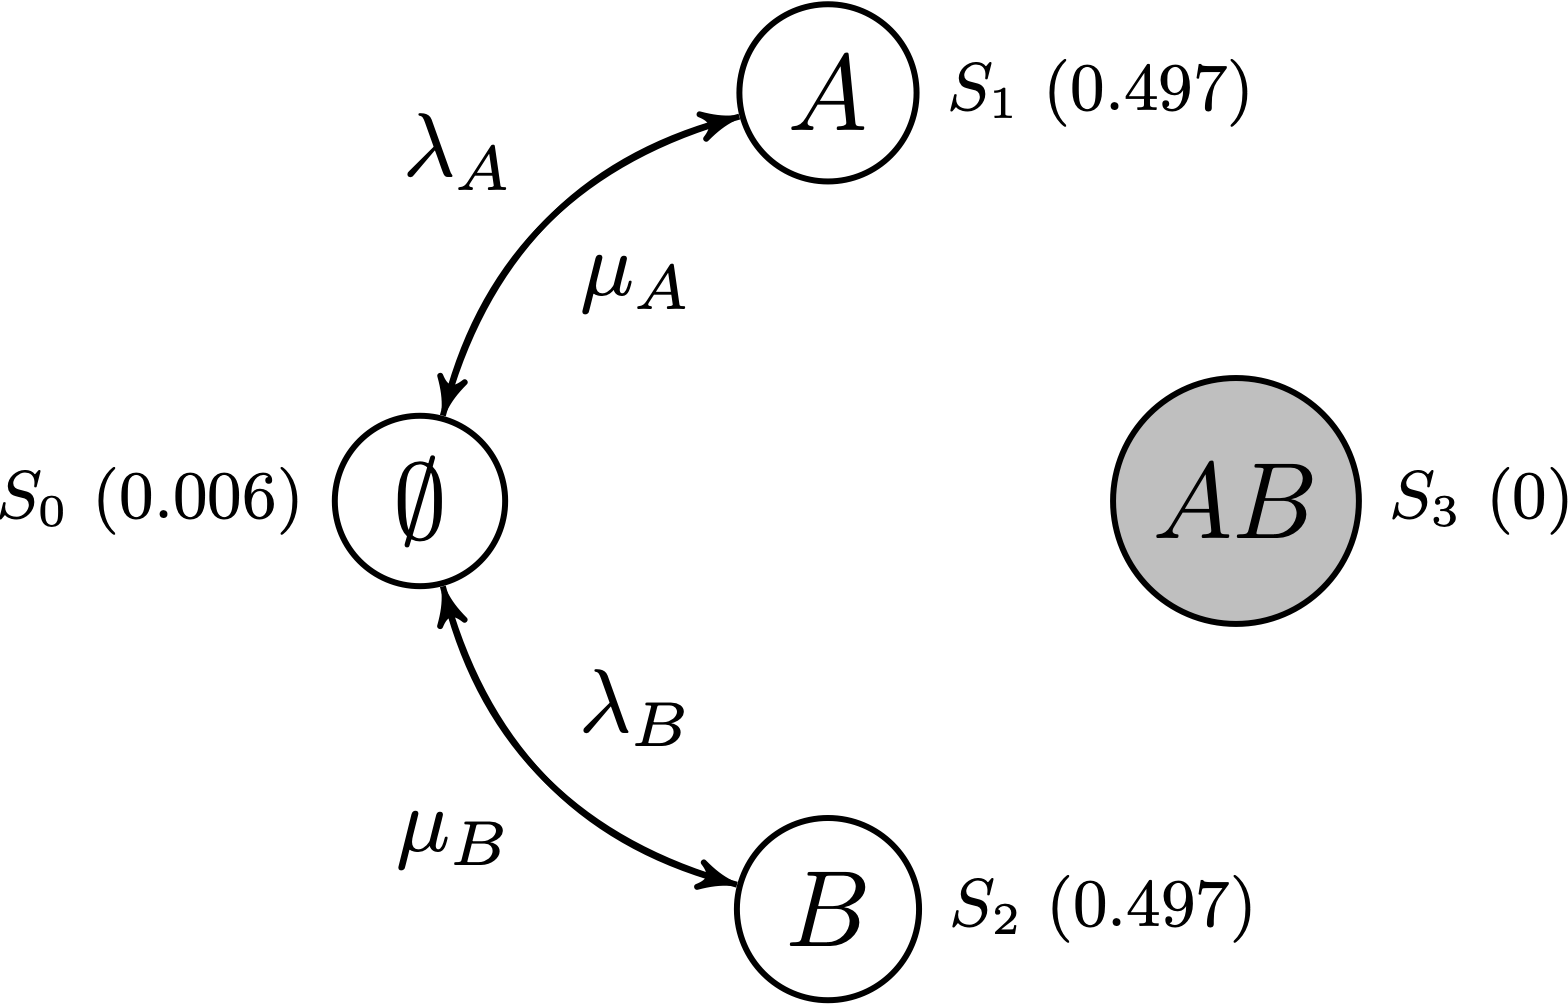
\includegraphics[width=0.4\textwidth]{ctmn_toy_scenario_1a}}\\
	% Situation 2
	\subfigure[Sensing area (OBSS/PD = -78 dBm)]{\label{fig:cs_toy_scenario_1b}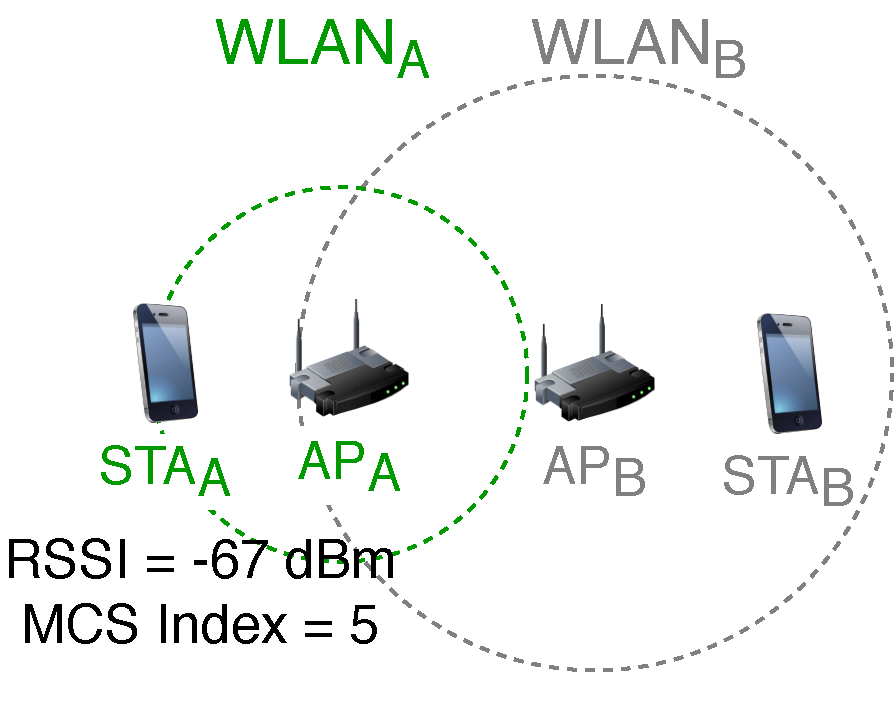
\includegraphics[width=0.4\textwidth]{fig_15c}}
	\hspace{1cm}
	% CTMN 2
	\subfigure[CTMN (OBSS/PD = -78 dBm)]{\label{fig:ctmn_toy_scenario_1b}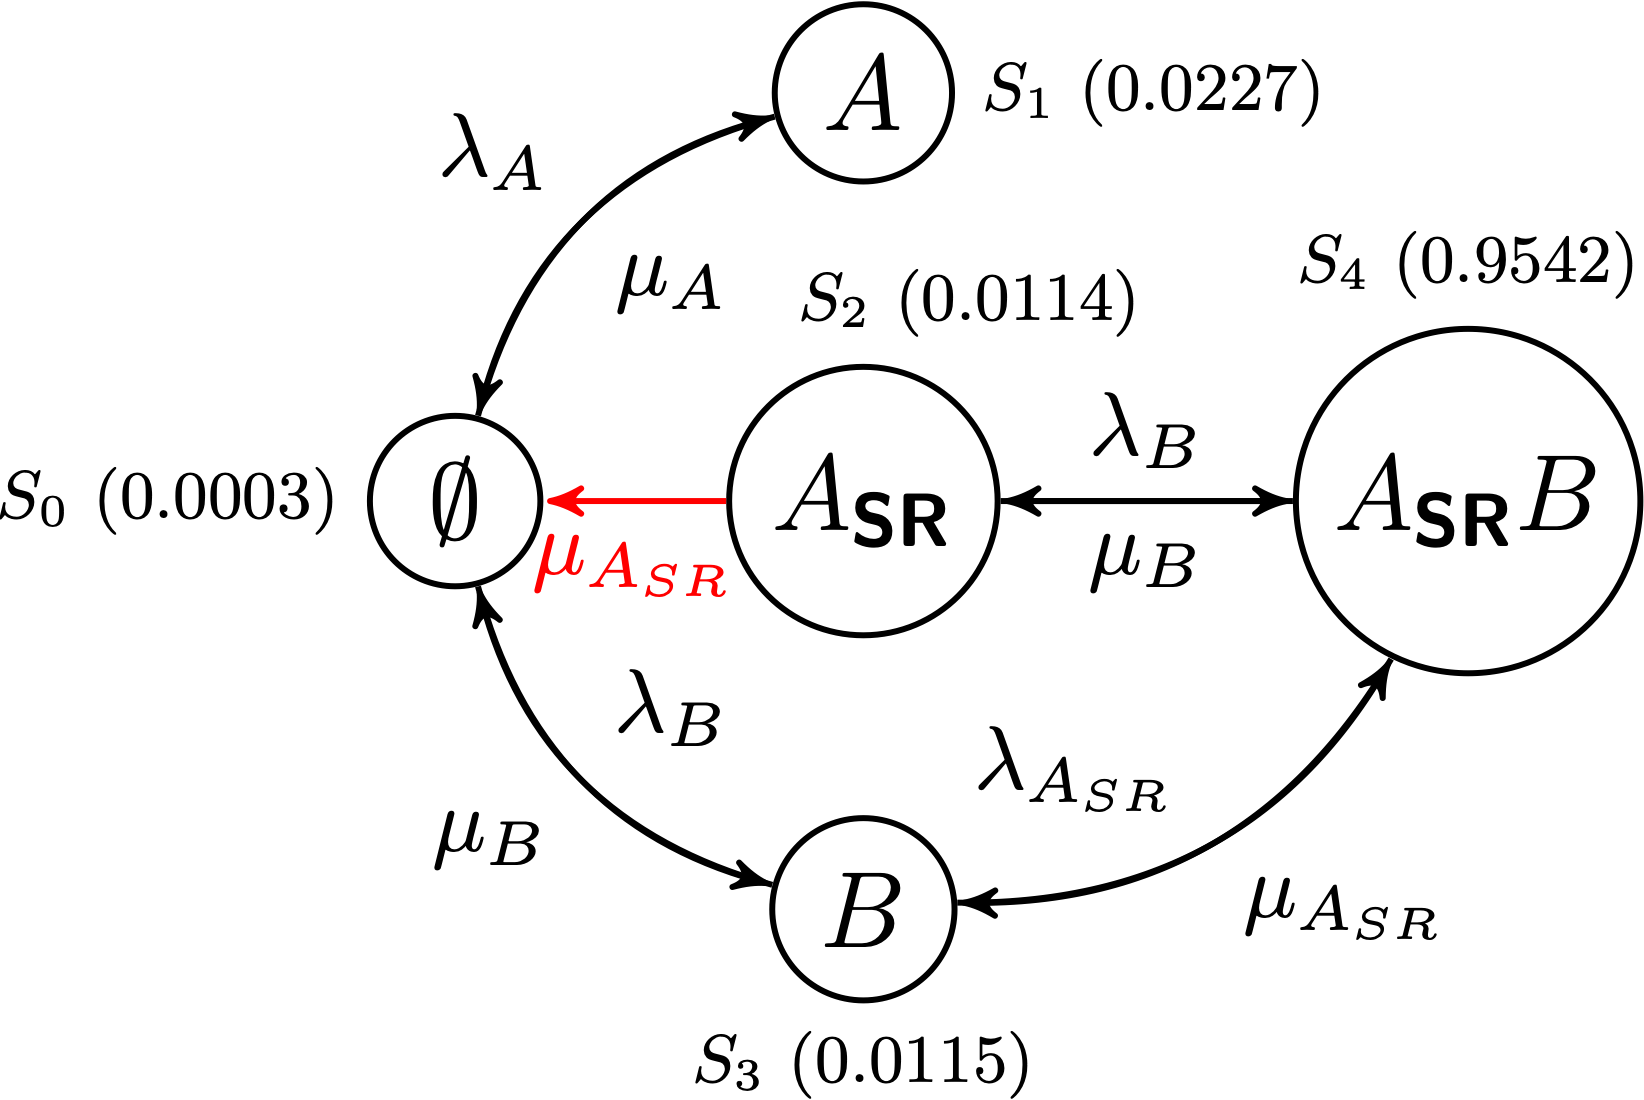
\includegraphics[width=0.4\textwidth]{ctmn_toy_scenario_1b}}%\\
	\caption{Representation of \emph{Toy scenario 1} for different settings. (a) and (c) illustrate the sensing area of each transmitter for CCA/CA = -82 dBm and OBSS/PD = -78 dBm, whereas (b) and (d) illustrate the corresponding inter-BSS interactions through CTMNs (unidirectional transitions are shown in red).}
	\label{fig:toy_scenario_1b}
\end{figure*}

As shown in Fig.~\ref{fig:cs_toy_scenario_1a} (CCA/CS is applied by both BSSs), $\text{AP}_\text{A}$ and $\text{AP}_\text{B}$ are in the carrier sense range of each other, and concurrent transmissions are not possible. This can also be noticed in the CTMN representation (see Fig.~\ref{fig:ctmn_toy_scenario_1a}), where state $s_3$ (AB) cannot be reached from any other state \textcolor{black}{(we hence represented it in gray) because of the continuous backoff assumption}. Nevertheless, both APs transmit at a high rate because the maximum power is used in isolation. %In particular, the STA in $\text{BSS}_\text{A}$ observes an RSSI of -64 dBm, which allows $\text{AP}_\text{A}$ using the MCS 7 for 20 MHz transmissions.

\textcolor{black}{When it comes to the SR setting, concurrent transmissions are possible, provided that $\text{BSS}_\text{A}$ uses an OBSS/PD value greater or equal than -79 dBm, which is the average power sensed from $\text{BSS}_\text{A}$. This is illustrated in Fig.~\ref{fig:cs_toy_scenario_1b}, where $\text{AP}_\text{A}$'s sensitivity area is reduced. In turn, ignoring inter-BSS transmissions entails a transmit power limitation. This results in poorer signal strength at the STA (RSSI = -67 dBm when the transmit power used by AP$_\text{A}$ is 17 dBm), thus requiring to use a more robust MCS. Fig.~\ref{fig:ctmn_toy_scenario_1b} shows the CTMN representation of the SR setting. Notice that new states (i.e. $s_2$ and $s_4$) appear as a result of applying SR in $\text{BSS}_\text{A}$ (denoted with subindex $\text{SR}$). It is worth pointing out that state $s_2$ ($A_\text{SR}$) can never be reached from the empty state ($s_0$). The fact is that $\text{BSS}_\text{A}$ can only use the SR mode after identifying an SR-based TXOP.}

\textcolor{black}{Fig.~\ref{fig:toy_scenario_1_results} shows the throughput achieved by $\text{BSS}_\text{A}$ and $\text{BSS}_\text{B}$, for each possible OBSS/PD value. The results have been obtained from both the SFCTMN and the Komondor simulator. The transmit power limitation that is imposed on each BSS is also illustrated (right side). As shown, both BSSs obtain the same performance for OBSS/PD $<$ -79 dBm because they share the channel on equal terms. To that point onwards, $\text{BSS}_\text{A}$ is able to ignore $\text{BSS}_\text{B}$'s transmissions and transmit concurrently. However, what might seem a worthy strategy for $\text{BSS}_\text{A}$ turns out to be more beneficial to $\text{BSS}_\text{B}$. The latter, except for OBSS/PD = -79 dBm,\footnote{At that point, the transmission power limitation for OBSS/PD = -79 dBm is insufficient, so $\text{BSS}_\text{B}$ senses the channel busy when $\text{BSS}_\text{A}$ transmits in SR mode.} enjoys the highest possible throughput when $\text{BSS}_\text{A}$ transmits after detecting an SR-based TXOP. The fact is that $\text{BSS}_\text{A}$ uses a lower transmission power than $\text{BSS}_\text{B}$.} As a result, $\text{BSS}_\text{B}$ will keep sensing the channel idle once its transmission finishes, provided that $\text{BSS}_\text{A}$ is still subject to the transmission power restriction.

\begin{figure}[ht!]
	\centering
	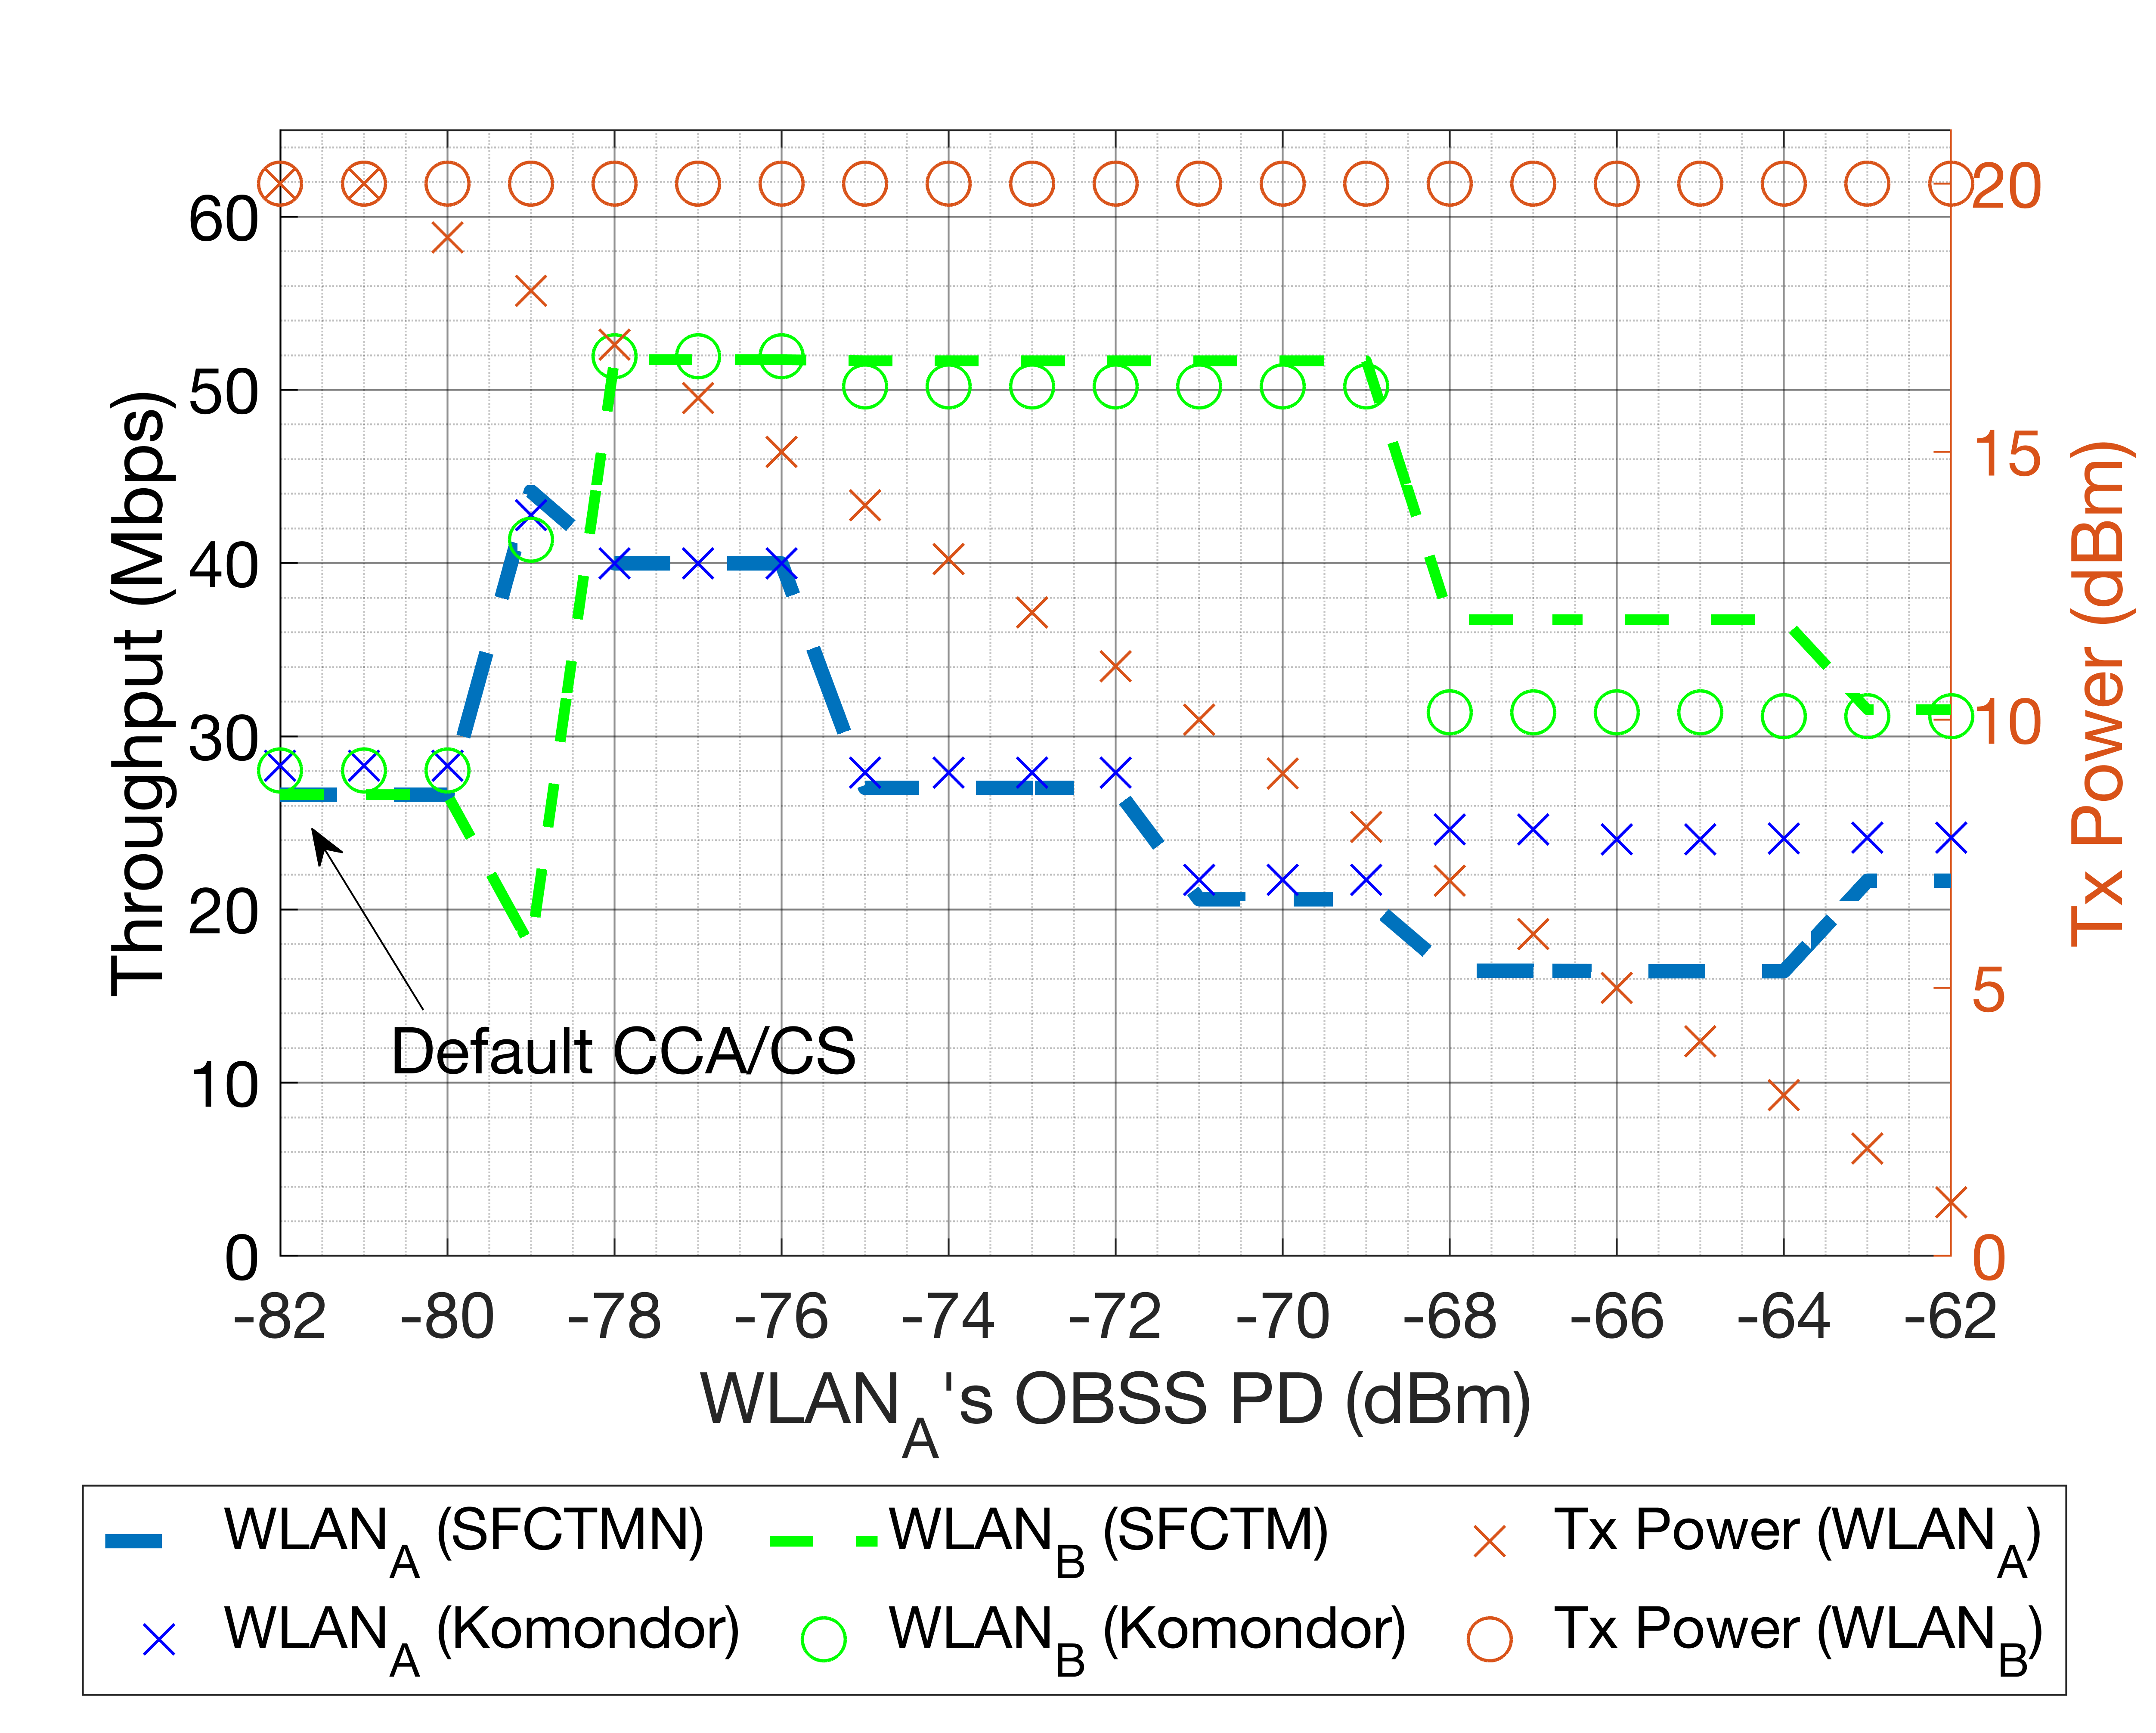
\includegraphics[width=.6\columnwidth]{SIM_1_1}
	\caption{Effects of applying OBSS/PD-based SR in $\text{BSS}_\text{A}$ of \emph{Toy scenario 1}, for each possible OBSS/PD value. The transmission power is shown in red. Results are shown for both SFCTMN and Komondor.}		\label{fig:toy_scenario_1_results}
\end{figure}

Apart from that, it is important to mention that there is a region (from OBSS/PD = -68 dBm to -64 dBm) in which the CTMN model is less accurate at capturing the actual SR behavior. The fact is that the CTMN model considers that the throughput obtained in every state is independent of the others, and this condition does not hold for states $A_\text{SR}B$ and $A_\text{SR}$. In reality, $\text{AP}_\text{A}$ is expected to abandon its transmission at state $A_\text{SR}B$ as soon as a timeout is noticed, thus spending a short time in SR mode (transition $A_\text{SR}B$ to $A_\text{SR}$ is unlikely). In contrast, the model considers that much more time is spent at state $A_\text{SR}$ since transmissions at that point are successful (but slow due to the low MCS used).
%For these OBSS/PD values, $\text{STA}_\text{A}$ cannot decode any transmission from $\text{AP}_\text{A}$ in state $A_\text{SR}B$. In turn, it can do that for the $A_\text{SR}$ state. In particular, the transmit power limitation used by $\text{AP}_\text{A}$ in the SR mode makes that $\text{STA}_\text{A}$ perceives an insufficient signal-to-noise-plus-interference ratio (SINR) when $\text{BSS}_\text{B}$ is also occupying the channel. 

Now, let us consider the case where both BSSs apply the SR operation. Fig.~\ref{fig:ctmn_toy_scenario_1c} shows the CTMN that illustrates the case in which concurrent transmissions between $\text{BSS}_\text{A}$ and $\text{BSS}_\text{B}$ (i.e., OBSS/PD $\geq$ -79 dBm) are possible. As shown, both BSSs can act by using the default or the SR modes, thus leading to a symmetric CTMN. In particular, we find two dominant states: $s_5$  and $s_6$. These states are visited with the same probability (0.4482), which indicates that both BSSs alternate the default and the SR modes. 

However, in reality, one of the BSSs may monopolize the channel \textcolor{black}{through} the default mode, while the other operates under the transmit power-constrained SR mode. This phenomenon is properly captured in the Komondor simulator, where SR-based TXOPs are identified on a per-packet basis. In this case, the BSS that accesses to the channel for the first time (e.g., $\text{BSS}_\text{A}$) is most likely to monopolize the channel. In contrast, \textcolor{black}{the other BSS (e.g., $\text{BSS}_\text{B}$) is prone to transmit under the SR mode} (as a result of $\text{BSS}_\text{A}$'s activity), until they alternate roles. Notice that either state $s_5$  or $s_6$ is more likely to be monopolized as the transmission time becomes longer than the idle periods. In our case, we have very long transmission times compared to the idle time since we assume full-buffer traffic, packet aggregation, and short Contention Window (CW) values.

\begin{figure}[ht!]
	\centering    
	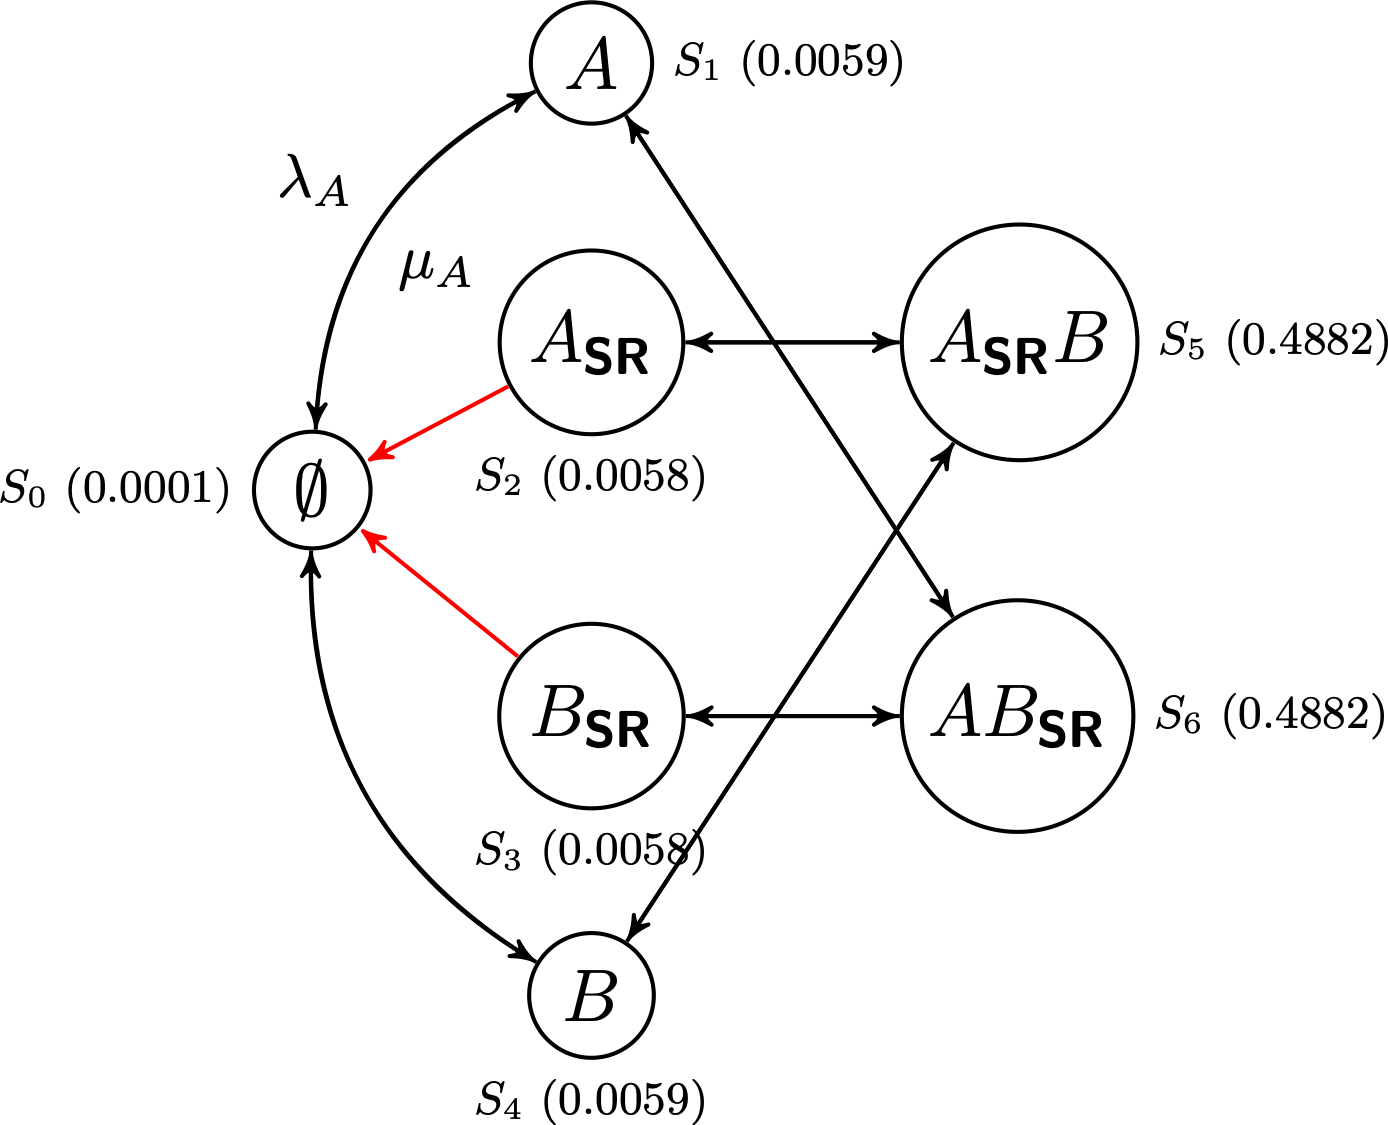
\includegraphics[width=.55\columnwidth]{ctmn_toy_scenario_1c}
	\caption{CTMN of \emph{Toy scenario 1} when both BSSs apply OBSS/PD-based SR with OBSS/PD~$\geq$~-79~dBm (unidirectional transitions are marked in red).}
	\label{fig:ctmn_toy_scenario_1c}
\end{figure}

%\begin{figure}[ht!]
%	\centering
%	\subfigure[CTMN representation]{\label{fig:ctmn_toy_scenario_1c}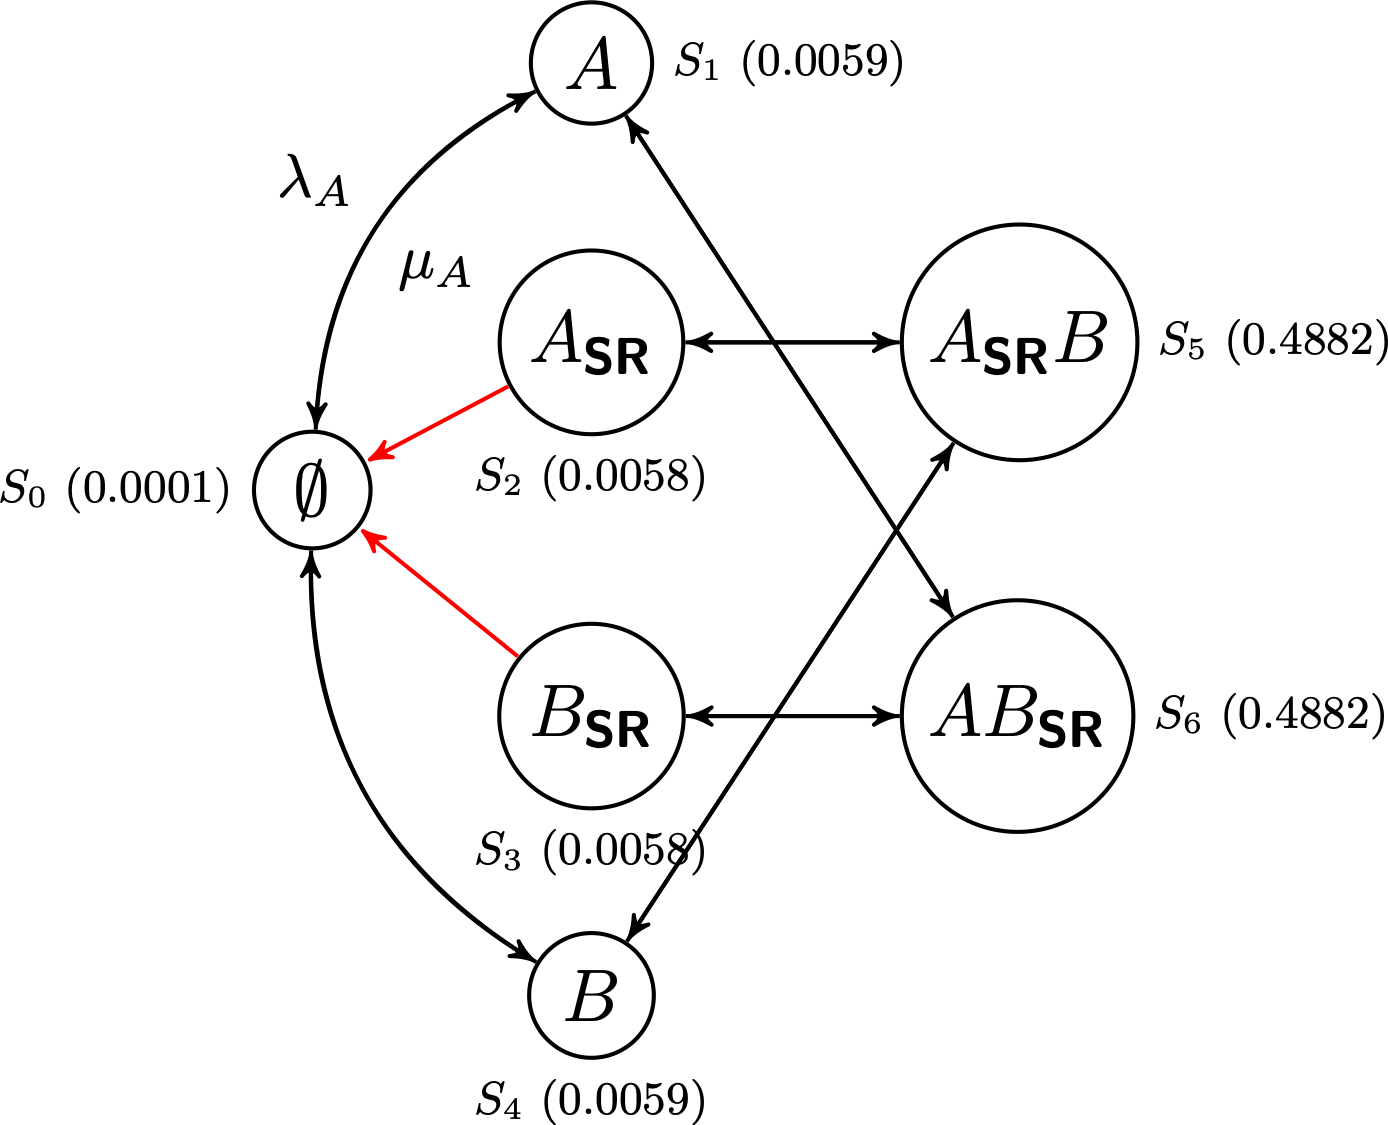
\includegraphics[width=.9\columnwidth]{ctmn_toy_scenario_1c}}
%	\subfigure[Throughput]{\label{fig:toy_scenario_1c_results}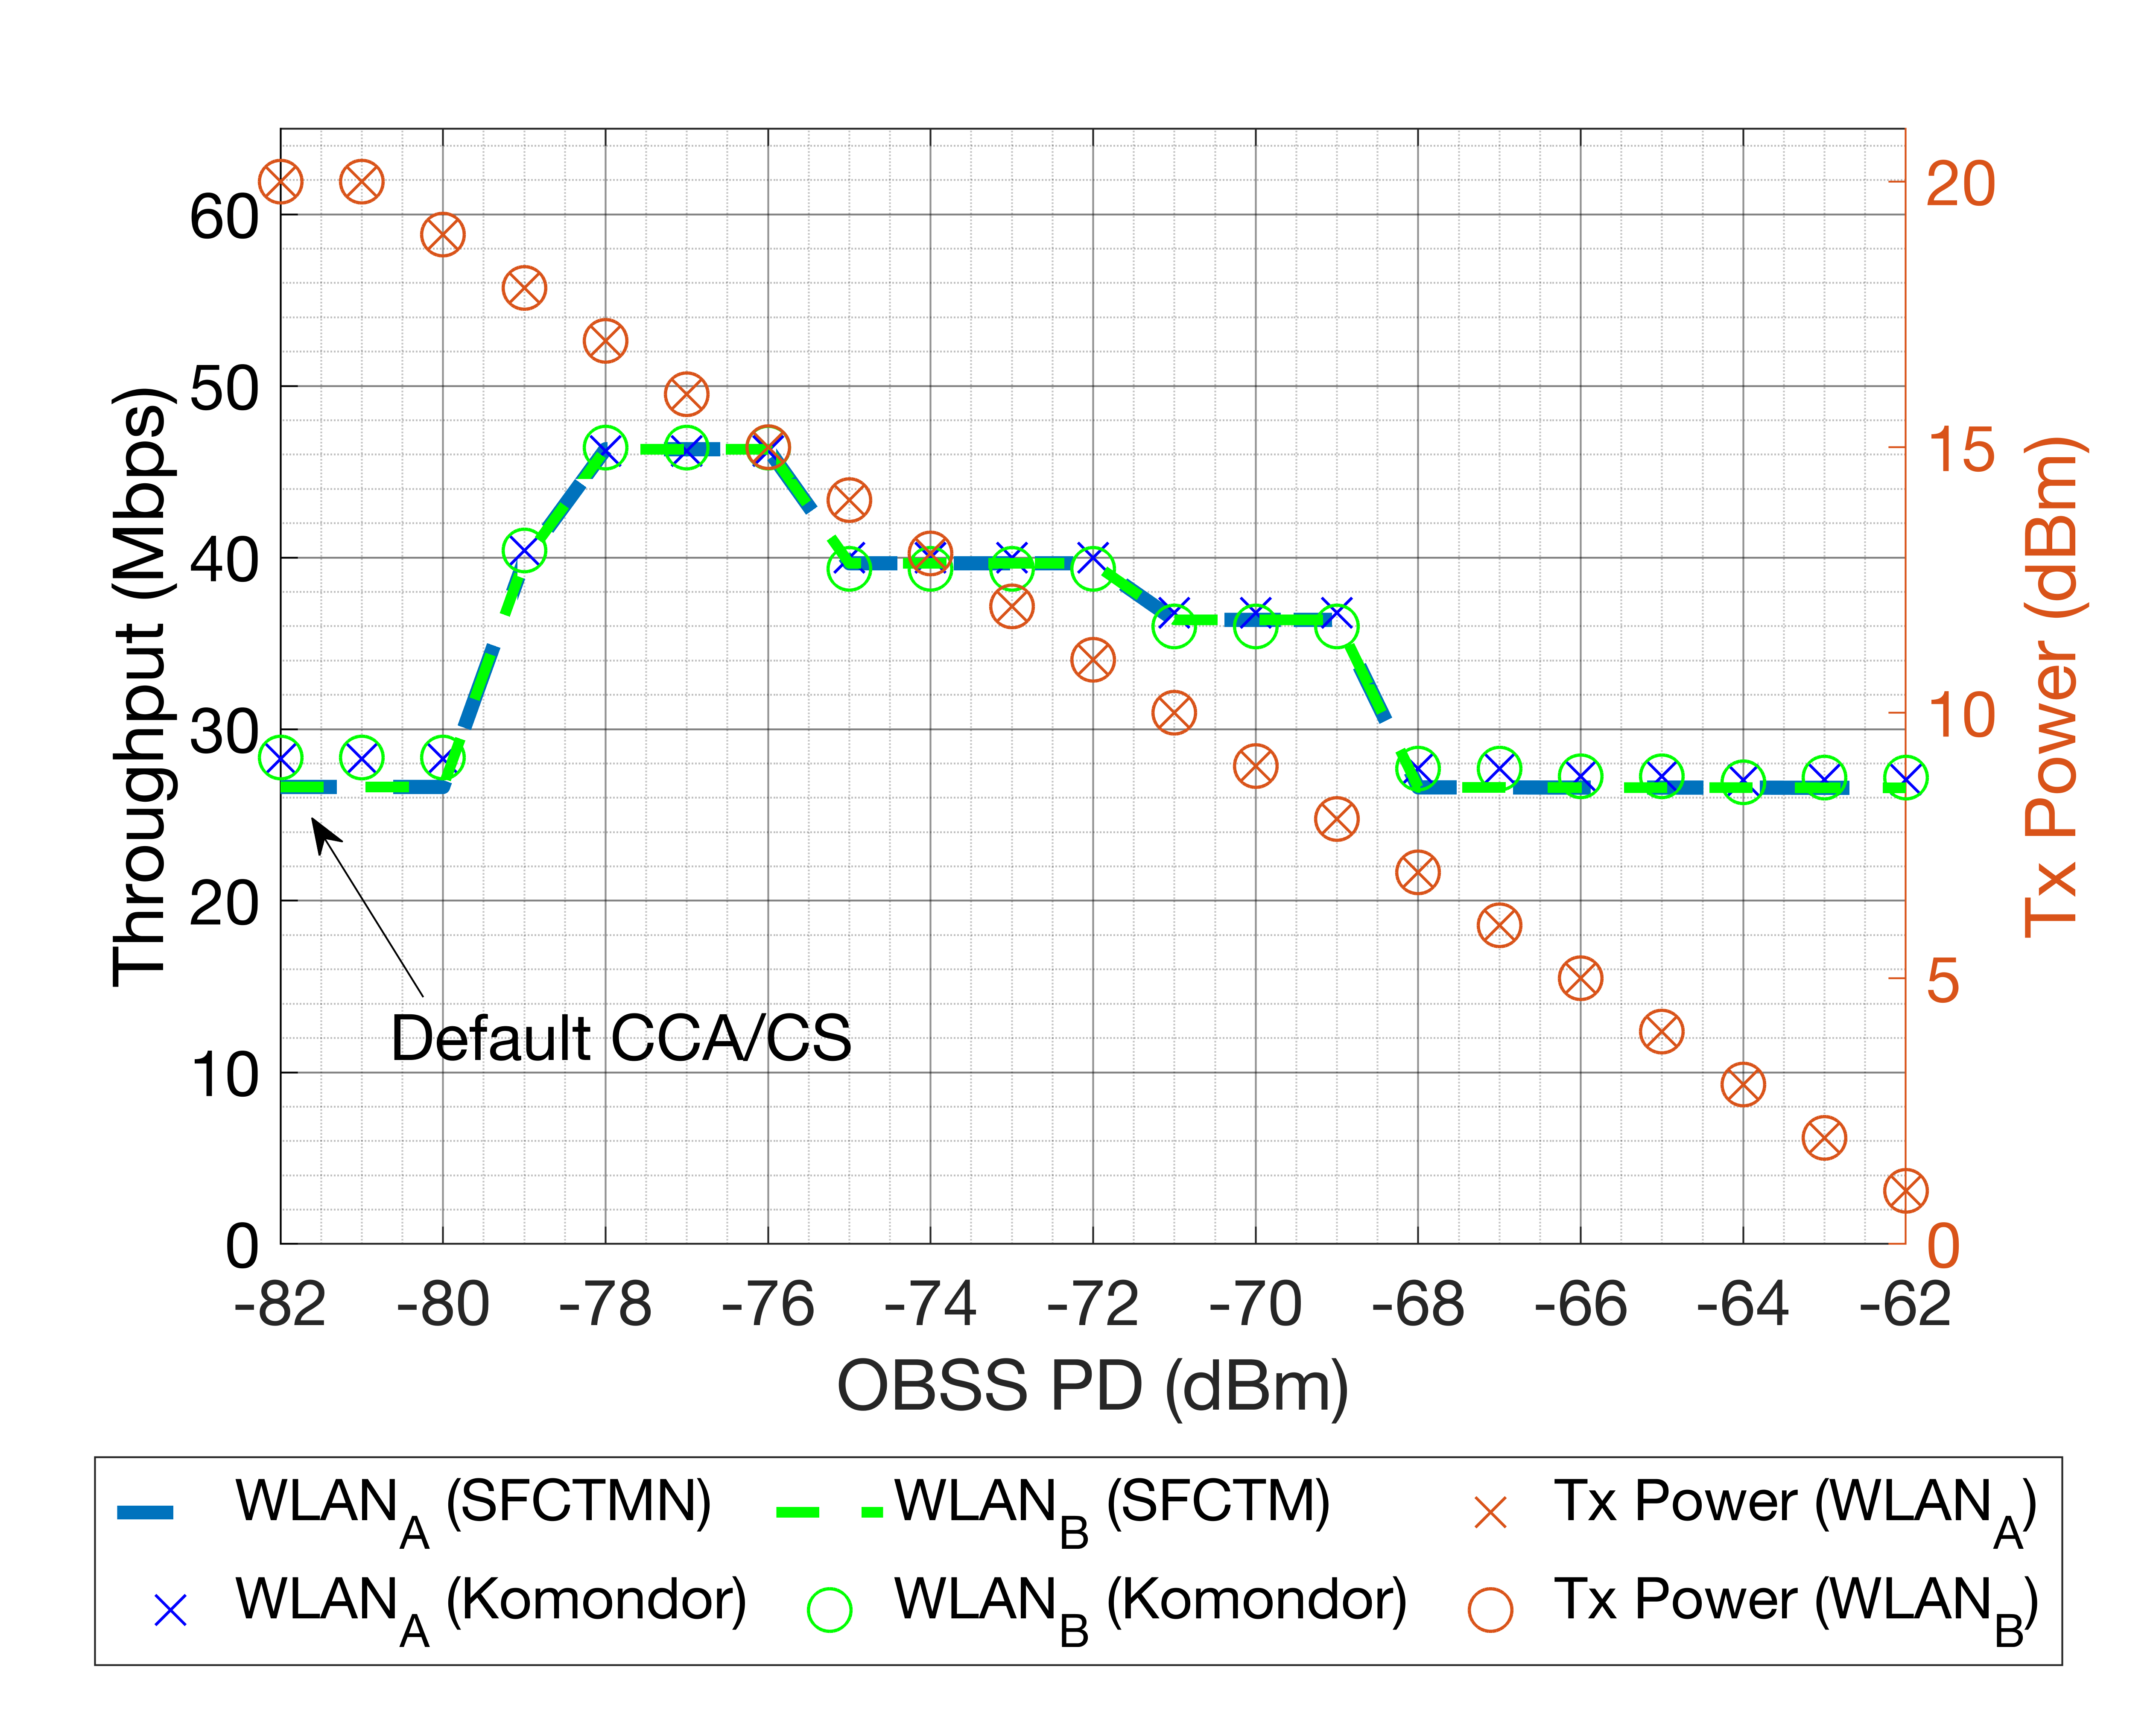
\includegraphics[width=\columnwidth]{SIM_1_1b}}
%	\caption{Effects of applying OBSS/PD-based SR in both BSSs of \emph{Toy scenario 1}. (a) CTMN for OBSS/PD~$\geq$~-79~dBm (unidirectional transitions are marked in red), and (b) throughput obtained for each OBSS/PD value. In (b), the transmission power is shown in red, and results are shown for both SFCTMN and Komondor.}
%	\label{fig:toy_scenario_1c}
%\end{figure}

Fig.~\ref{fig:toy_scenario_1c_results} shows the throughput achieved by each BSS when both apply SR, and for each OBSS/PD threshold. Again, the results have been extracted from both SFCTMN and Komondor. In order to show the long-term performance of each BSS in the Komondor simulator, we have displayed the average values obtained from 100 simulations. As shown, the performance achieved by both BSSs is totally fair, due to the symmetry of the scenario. In particular, states in which SR is used are alternated, thus allowing each BSS to access the channel while the other is transmitting. As a result, the \textcolor{black}{aggregate throughput} can be further increased with respect to the case in which only one BSS applies SR. %However, unlike the previous case, the long-term individual throughput never reaches the maximum possible throughput in isolation (the transmission power limitation prevents to do so).

\begin{figure}[ht!]
	\centering
	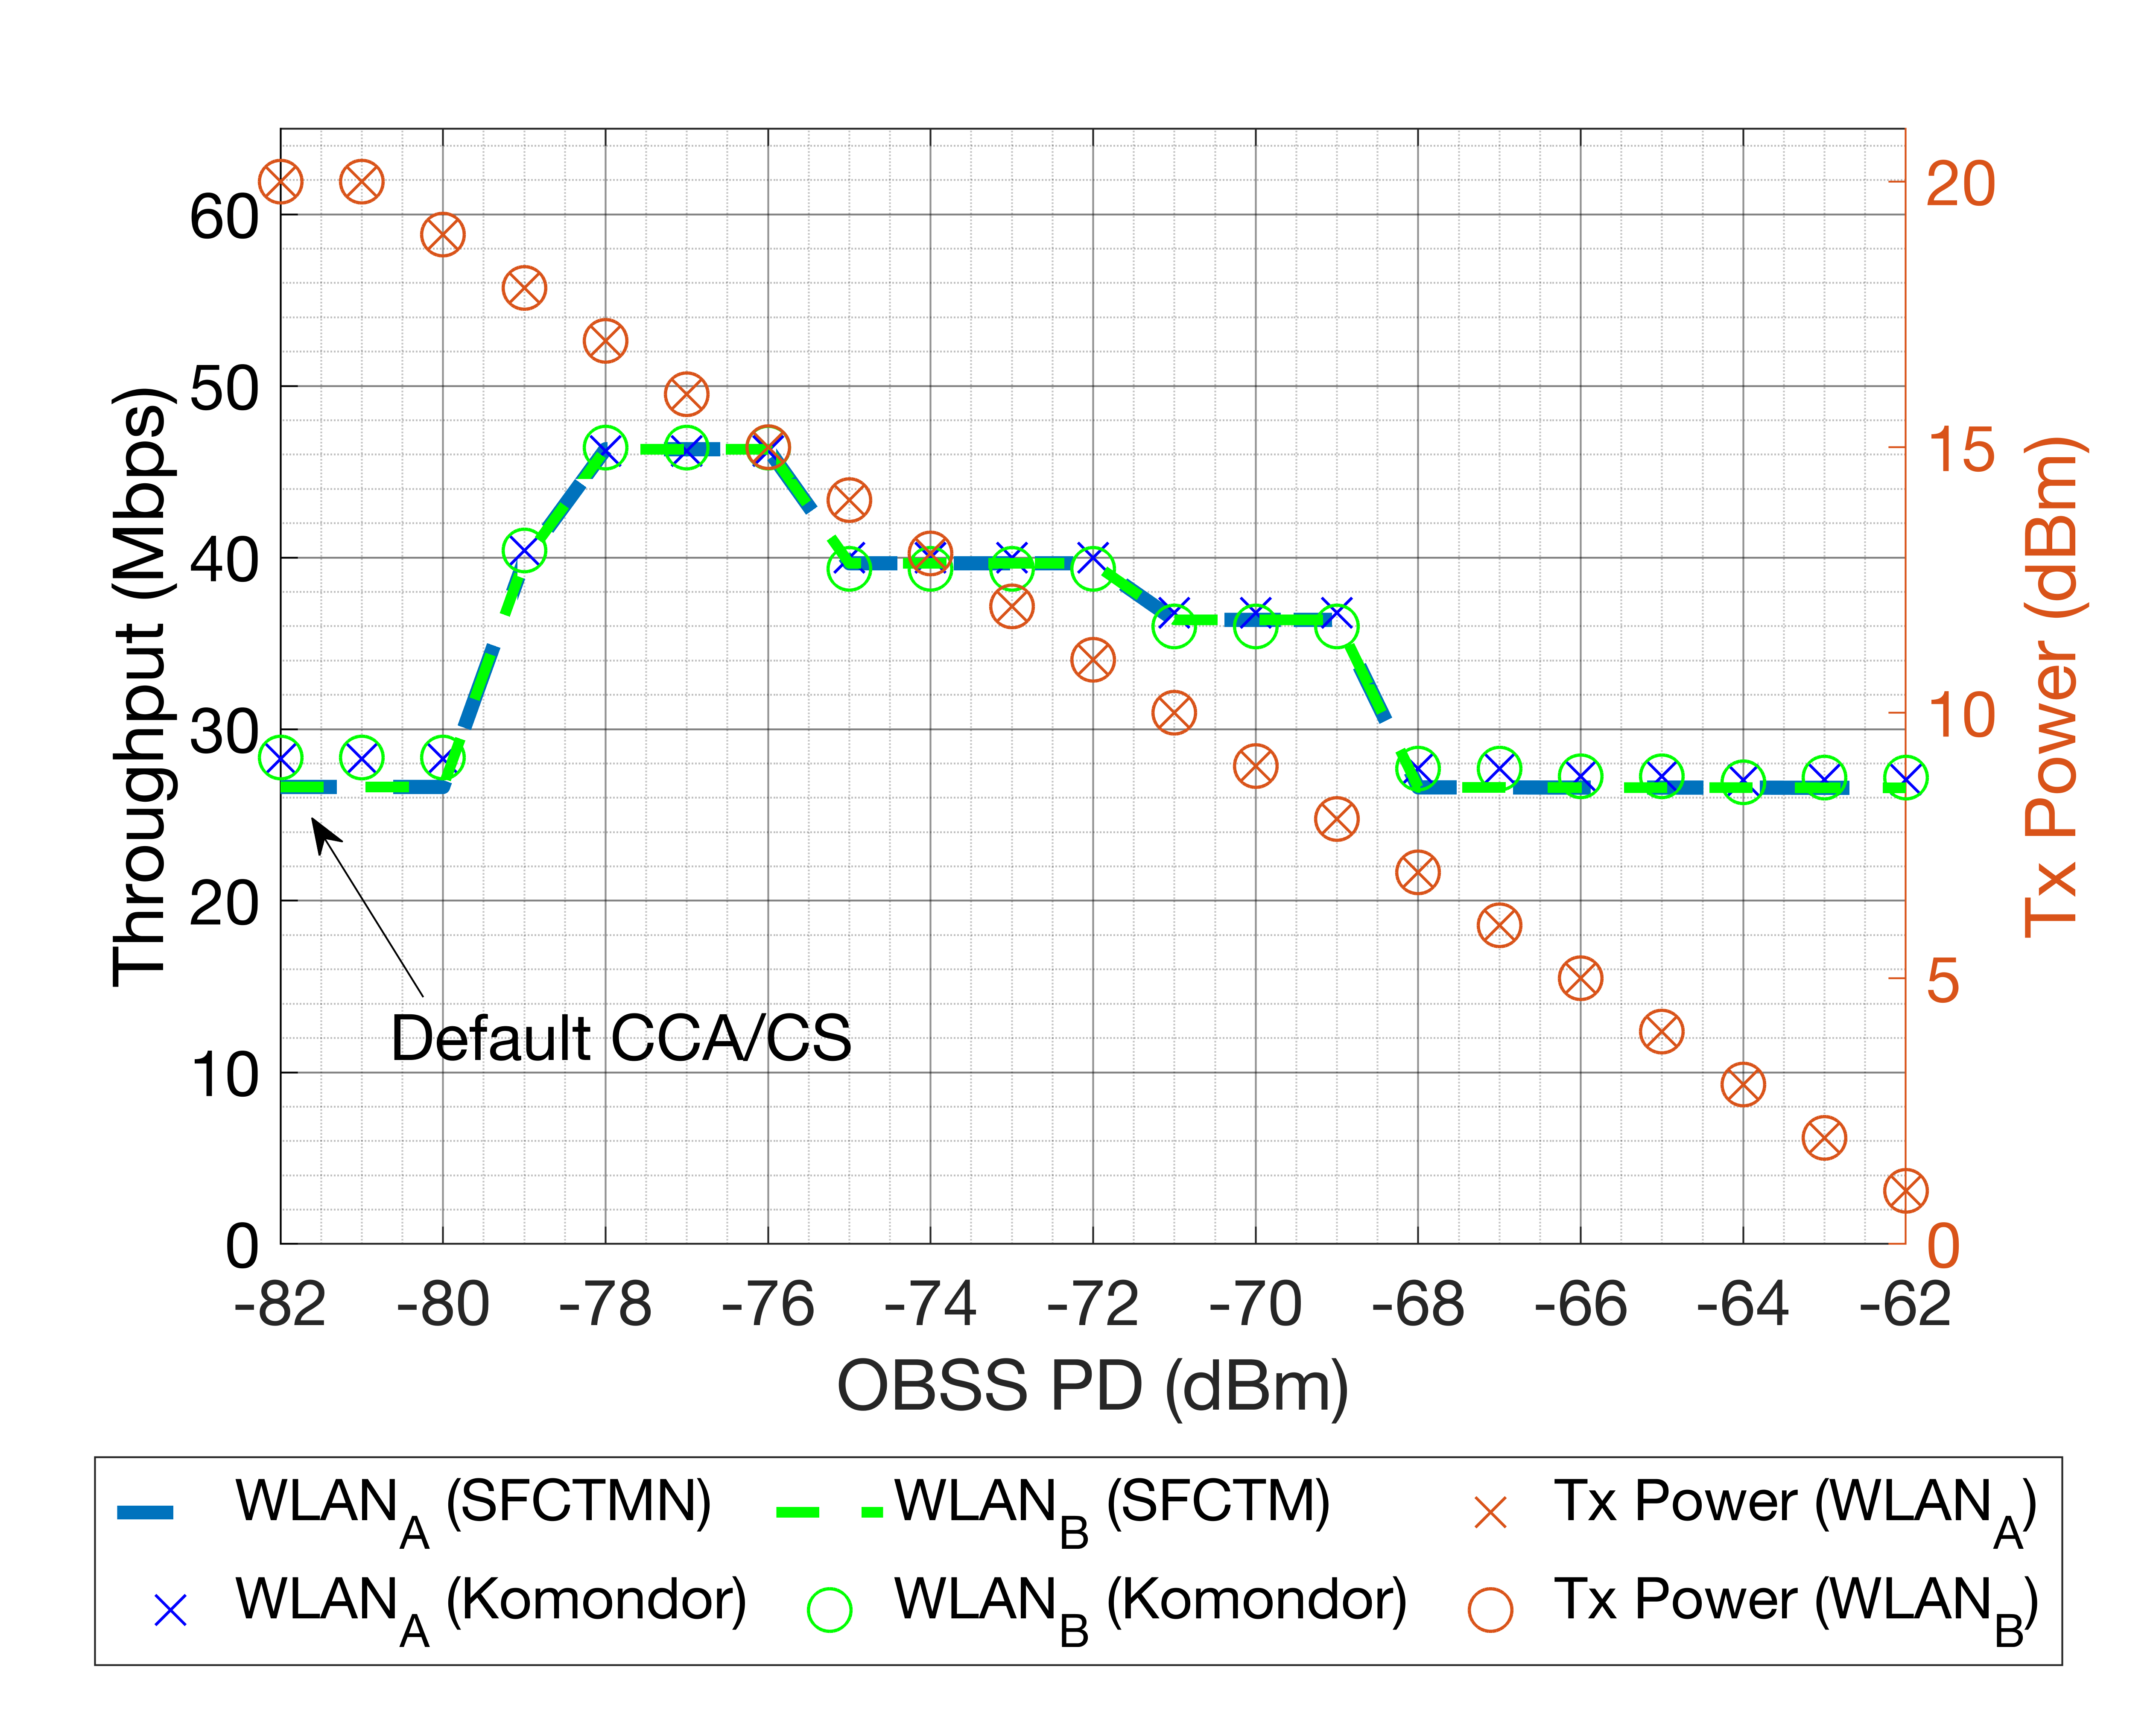
\includegraphics[width=.6\columnwidth]{SIM_1_1b}
	\caption{Effects of applying OBSS/PD-based SR in both BSSs of \emph{Toy scenario 1}, for each possible OBSS/PD value. The transmission power is shown in red. Results are shown for both SFCTMN and Komondor.}		
	\label{fig:toy_scenario_1c_results}
\end{figure}

%%% Complex OBSS/PD-based interactions
\subsection{Interactions among Spatial Reuse groups}
\label{section:advanced_interactions}
Differentiating between SRGs may potentially enhance spectral efficiency. In practice, devices belonging to the same SRG use a dedicated OBSS/PD threshold, namely SRG OBSS/PD. For the rest of inter-BSS transmissions, the non-SRG OBSS/PD threshold is used instead. One possible use case may lie in residential building apartments, where BSSs belonging to the same building form an SRG. For the rest of networks (e.g., public Wi-Fi in the street), other SRGs can be considered. 

To illustrate the implications of using SR with SRGs, let us focus on \emph{Toy scenario 2}, which is depicted in Fig.~\ref{fig:toy_scenario_2}. In this deployment, all the BSSs apply the SR operation and two different SRGs are created. In particular, BSSs belonging to the same SRG (i.e., $\text{BSS}_\text{A}$ and $\text{BSS}_\text{B}$) are close to each other, such as in a residential building. Apart from that, $\text{BSS}_\text{C}$, belongs to another SRG. Fig.~\ref{fig:SIM_1_3_individual} shows the individual and max-min\footnote{The max-min throughput corresponds to the solution that maximizes the minimum throughput achieved by a set of BSSs.} throughput obtained by jointly applying OBSS/PD-based SR in \emph{Toy scenario 2}. \textcolor{black}{Notice that we have considered that all the BSSs in the same SRG apply the same OBSS/PD value} since the number of total combinations grows exponentially and is unfeasible to be plotted. 

\begin{figure}[ht!]
	\centering
	\subfigure[Scenario]{\label{fig:toy_scenario_2}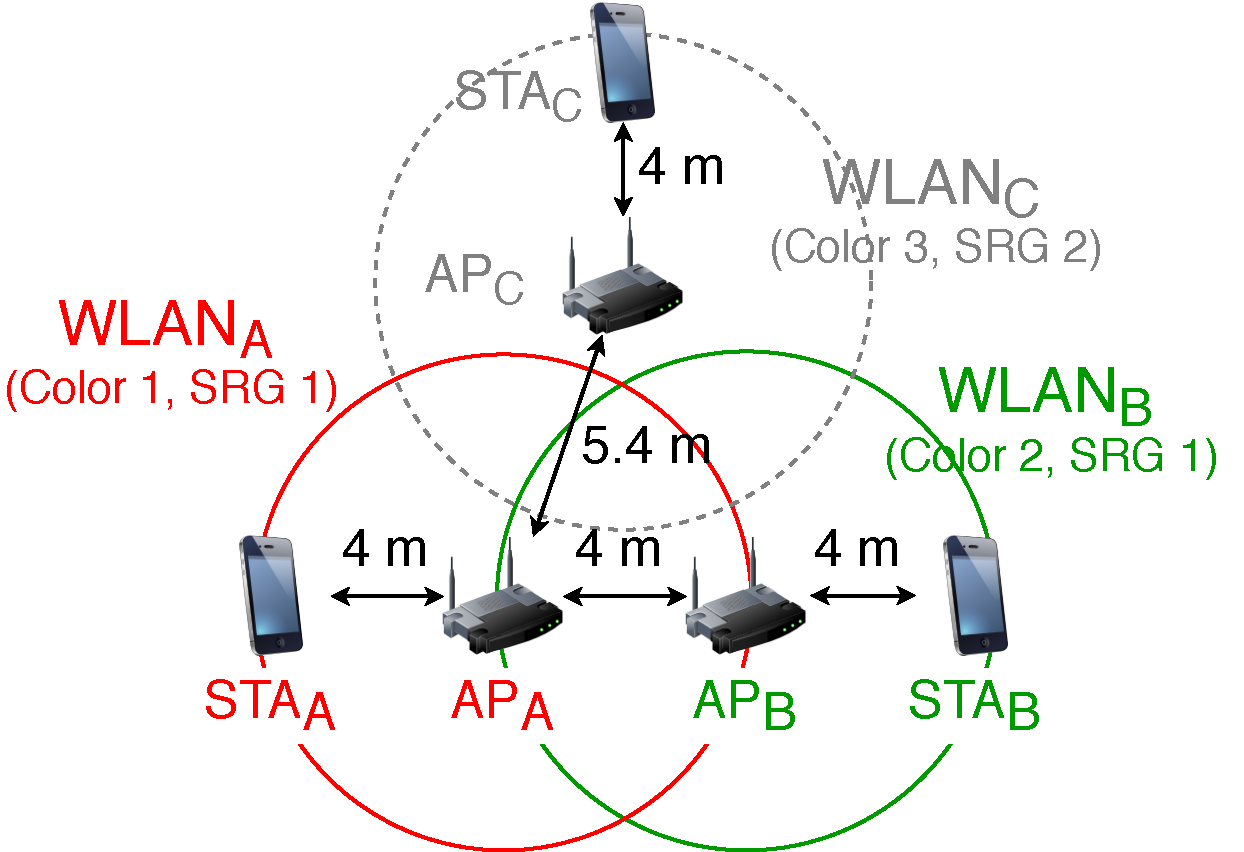
\includegraphics[width=0.4\columnwidth]{fig_18}}
	\hspace{1cm}
	\subfigure[Results]{\label{fig:SIM_1_3_individual}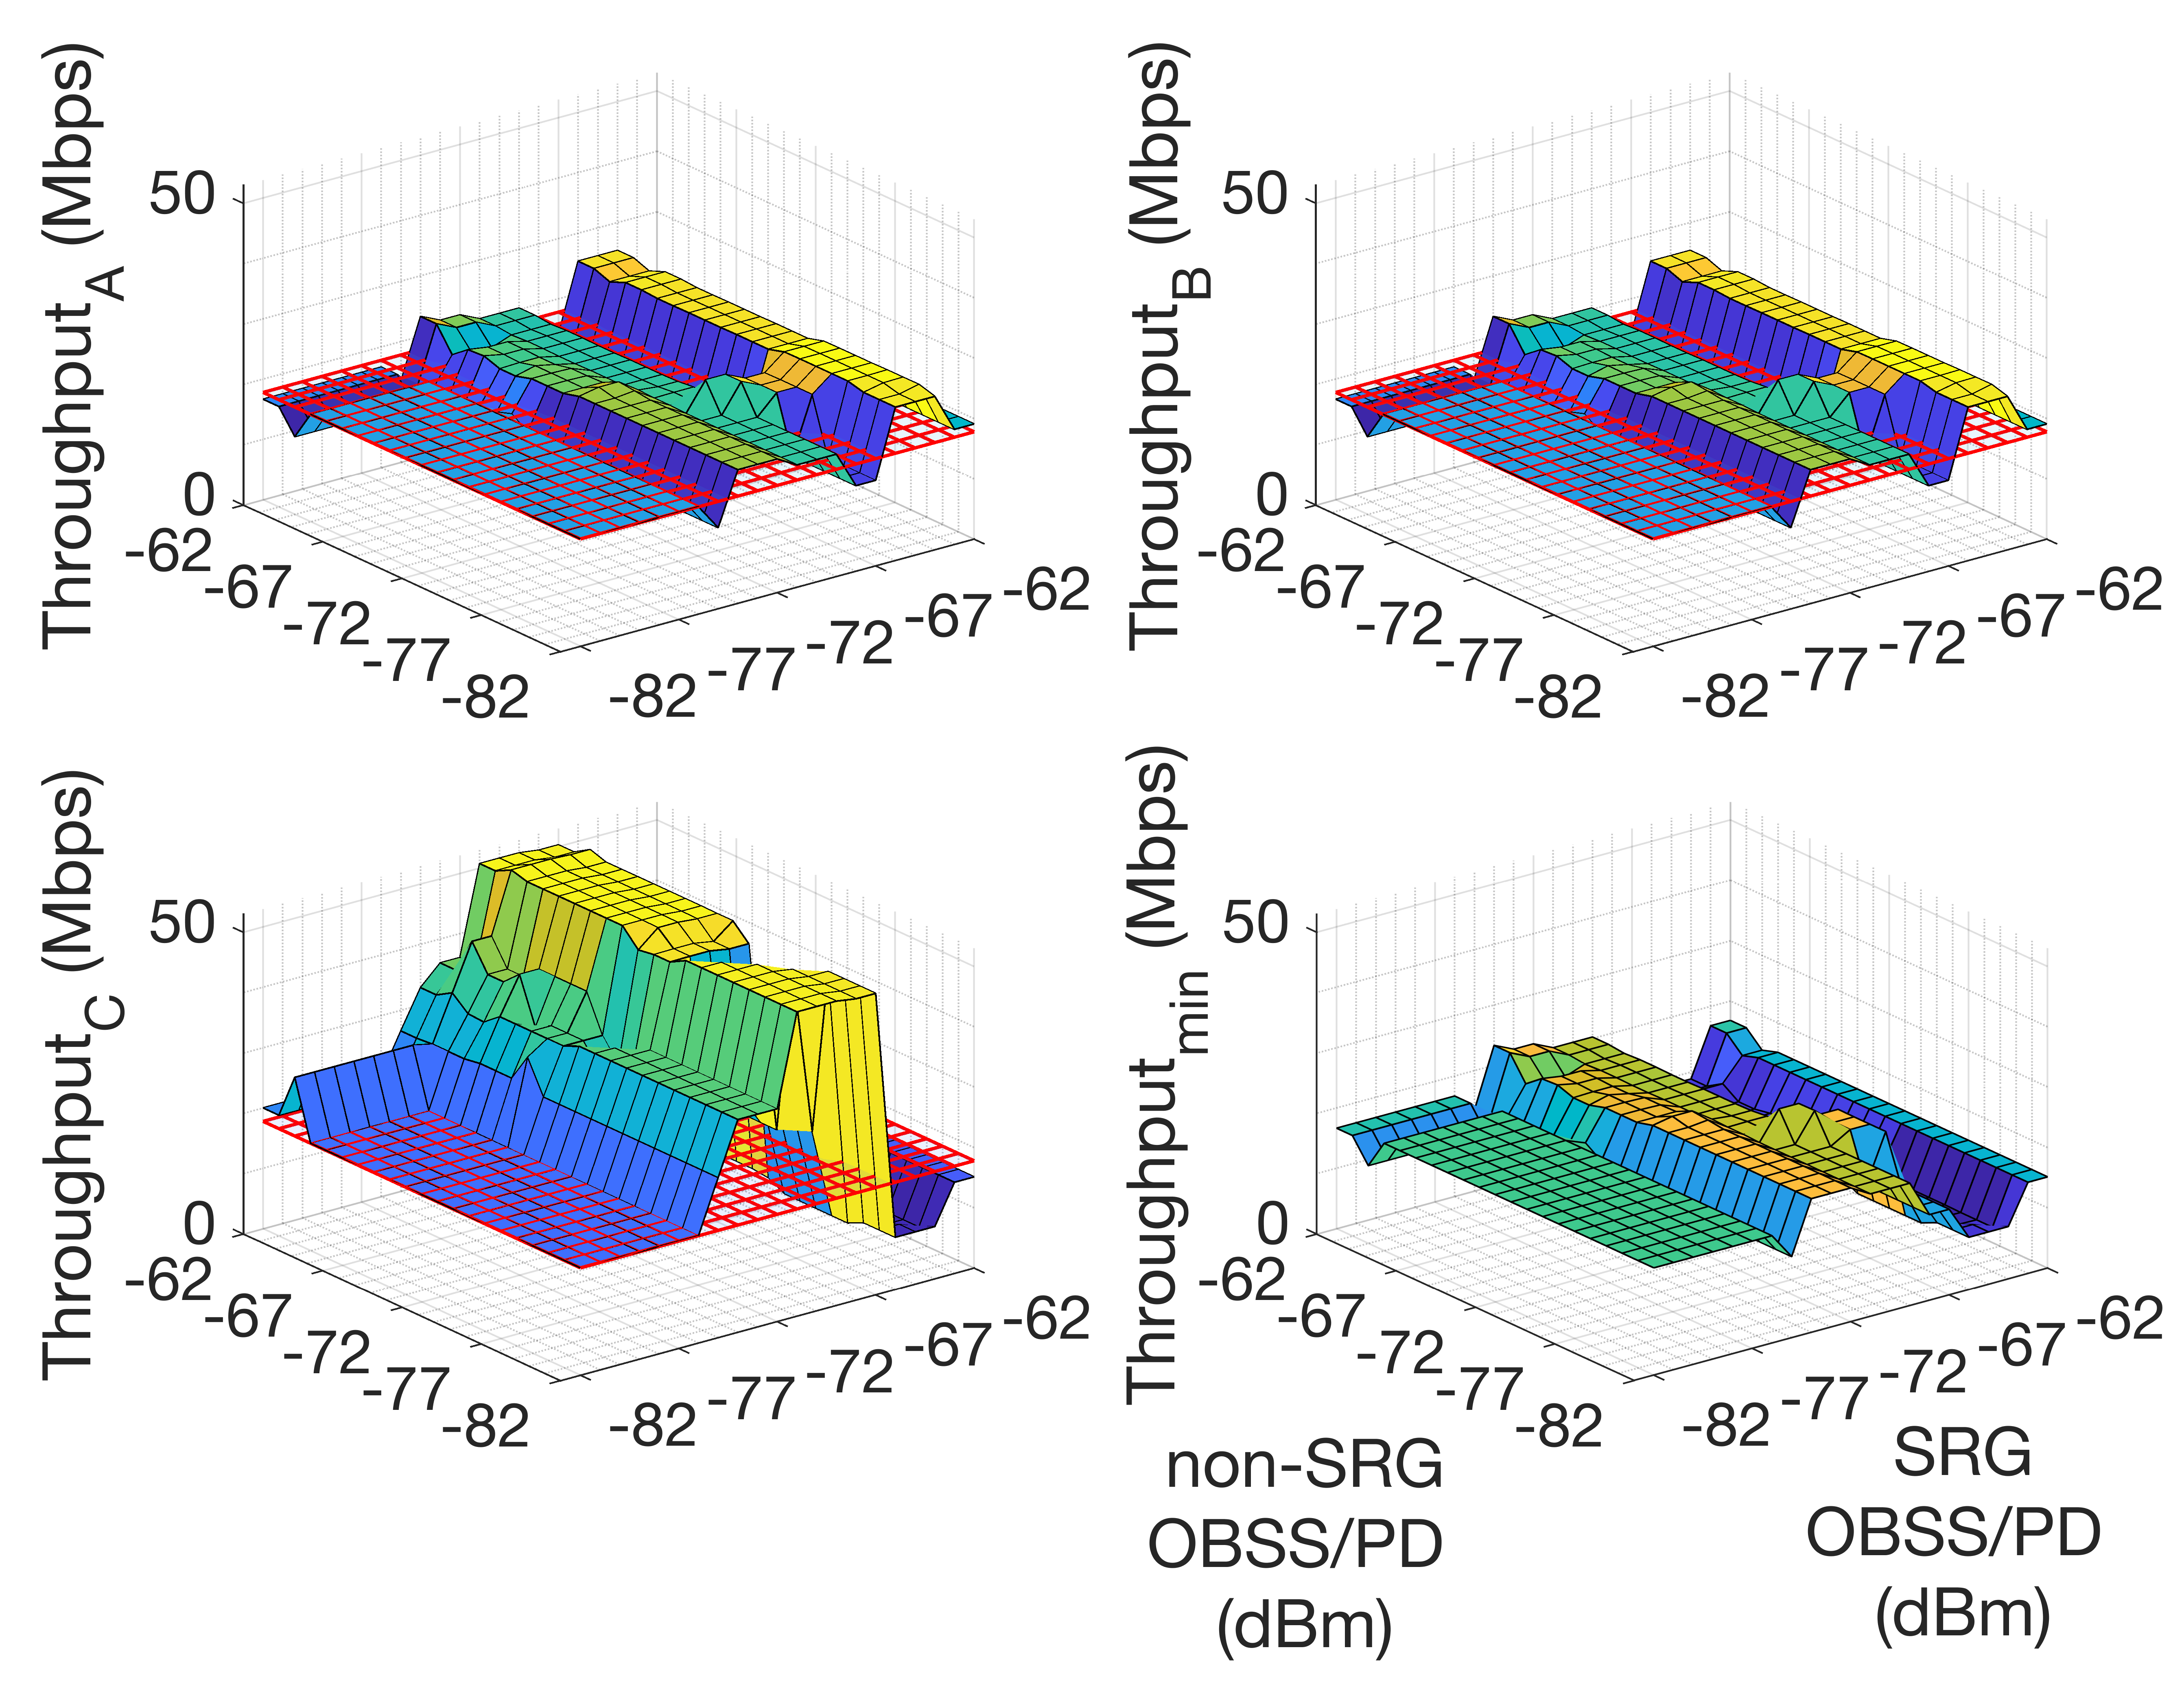
\includegraphics[width=.5\columnwidth]{SIM_1_2}}
	\caption{Results of applying the OBSS/PD-based SR operation in \emph{Toy scenario 2}. In (b), the individual and max-min throughput are shown for each SRG and non-SRG OBSS/PD threshold. The red mesh indicates the performance achieved by using the default CCA/CS.}
	\label{fig:fig:17}
\end{figure}

\begin{figure}[ht]
	\centering
	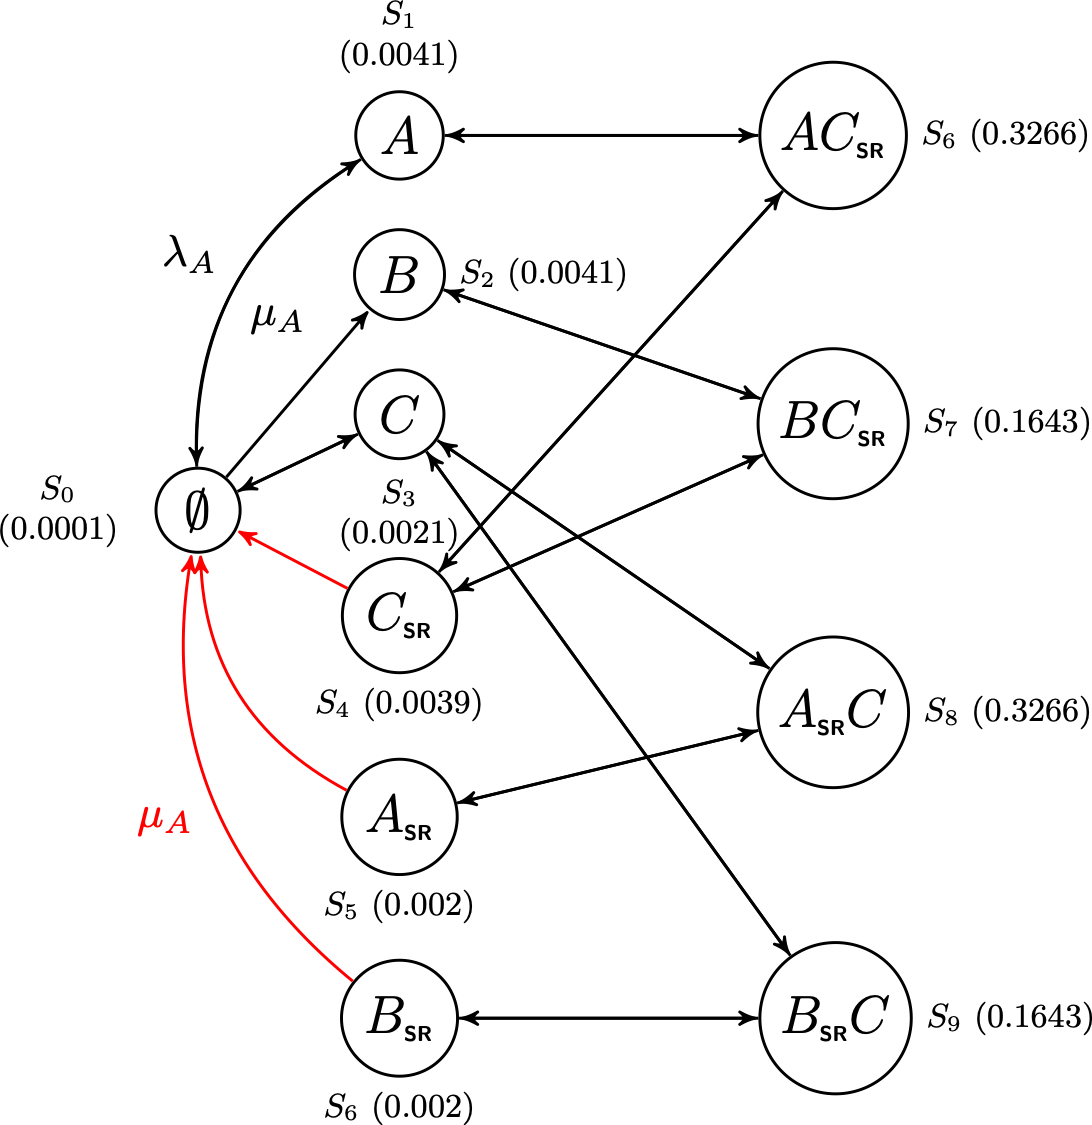
\includegraphics[width=.5\columnwidth]{ctmn_scenario_2}
	\caption{CTMN of \emph{Toy scenario 2}, for non-SRG OBSS/PD = -73 dBm and SRG OBSS/PD = -82 dBm. The unidirectional transitions are marked in red, and subindex \emph{SR} indicates the use of the non-SRG OBSS/PD threshold.}
	\label{fig:ctmn_scenario_2}
\end{figure}

As shown, the throughput achieved by each BSS follows an irregular pattern due to the complex inter-BSS interactions that take place in this scenario. Also, it can be appreciated the clashing interests of each BSS, where the individual performance is sometimes maximized at the expense of reducing the throughput of the others. For instance, if we focus on $\text{BSS}_\text{C}$, it obtains the maximum throughput when flow starvation is generated to $\text{BSS}_\text{A}$ (the same occurs for $\text{BSS}_\text{B}$). However, this is not optimal in terms of fairness. The CTMN resulting from the flow starvation situation is shown in Fig.~\ref{fig:ctmn_scenario_2}, which is given when all the BSSs use non-SRG OBSS/PD = -82 dBm and SRG OBSS/PD = -73 dBm.\footnote{The CTMN model captures the utilization of different OBSS/PD thresholds by considering that each BSS acts in three different ways (states), as a result of the employed OBSS/PD threshold: \emph{i)} default CCA/CS, \emph{ii)} SRG OBSS/PD, and \emph{iii)} non-SRG OBSS/PD.}

\textcolor{black}{Concerning} the optimal max-min performance, we notice that it is optimized when all the BSSs can ignore every single detected inter-BSS transmission (regardless of its source). This situation is fair and, at the same time, increases the overall performance. However, it occurs when all the inter-BSS transmissions are equally treated. Using SRGs can improve the performance of specific nodes (from a single group), but potentially leads to unfairness. 

Table \ref{tbl:cross_validation} verifies the results obtained in \emph{Toy scenario 2} from both SFCTMN and Komondor. For the sake of representation, we show the Root Mean Square Error (RMSE) for all the considered SRG and non-SRG OBSS/PD thresholds. As shown, the error for $\text{BSS}_\text{A}$ and $\text{BSS}_\text{B}$ is relatively small. In contrast, a higher error is obtained for $\text{BSS}_\text{C}$. This is strongly related to the fact that $\text{BSS}_\text{C}$ belongs to a different SRG than $\text{BSS}_\text{A}$ and $\text{BSS}_\text{B}$, which leads to different inter-BSS interactions. Moreover, dominant states may lead to situations that cannot be captured by the SFCTMN, as previously shown for \emph{Toy scenario 1}. In particular, $\text{BSS}_\text{C}$ in \emph{Toy scenario 2} is prone to participate in these states because of its asymmetric location with respect to $\text{BSS}_\text{A}$ and $\text{BSS}_\text{B}$.
\begin{table}[ht!]
	\centering
		\begin{tabular}{|c|c|c|c|}
			\hline
			& $\text{BSS}_\text{A}$ & $\text{BSS}_\text{B}$ & $\text{BSS}_\text{C}$ \\ \hline
			\begin{tabular}[c]{@{}c@{}}RMSE \\ (Mbps)\end{tabular} & 6.02 & 6.03 & 18.42 \\ \hline
	\end{tabular}
	\caption{Verification of the results obtained in \emph{Toy scenario 2} from the SFCTMN and Komondor.}
	\label{tbl:cross_validation}
\end{table}

% ----------------------------------
% -
% 	-- Performance Evaluation --
% -
% ----------------------------------

\section{Performance Evaluation}
\label{section:performance_evaluation}

In this Section, we study the performance gains of SR in large-scale WLAN scenarios. To that purpose, we leave the CTMNs-based analysis out and concentrate on simulation results. For the rest of this Section, each BSS is considered to be composed by an AP and a single STA, which are placed uniformly at random, as shown in Fig.~\ref{fig:random_scenario}. 

\begin{figure}[ht!]
	\centering
	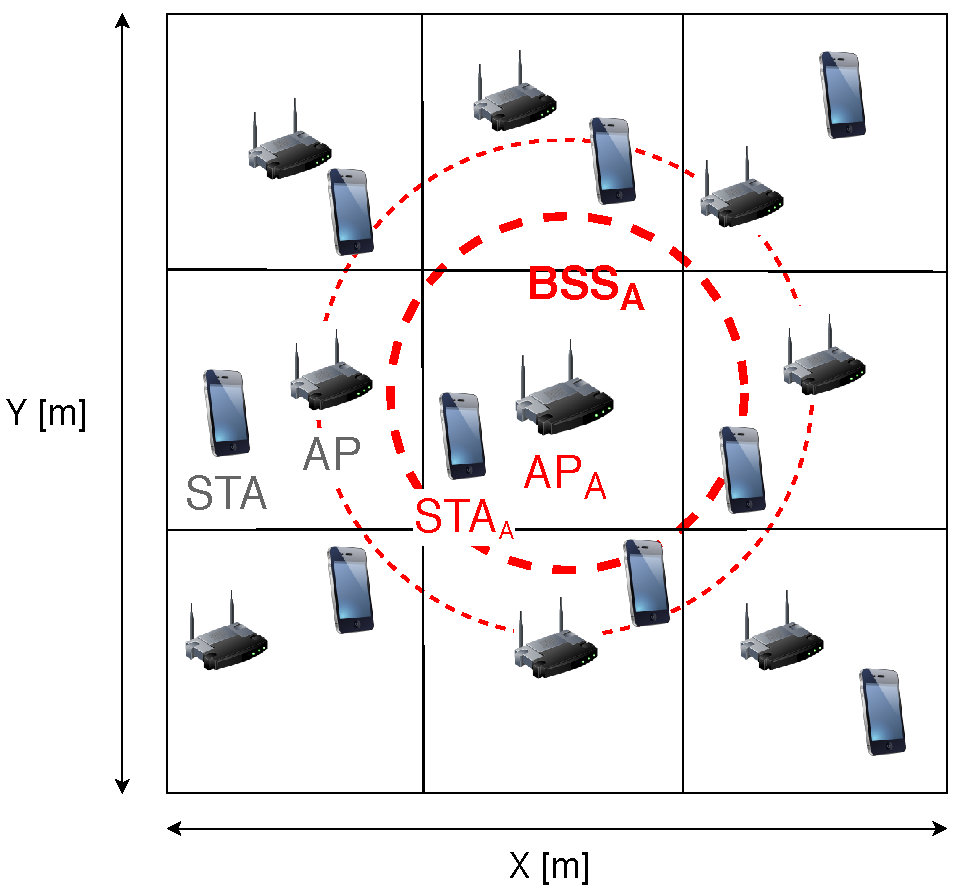
\includegraphics[width=0.45\columnwidth]{random_scenario}
	%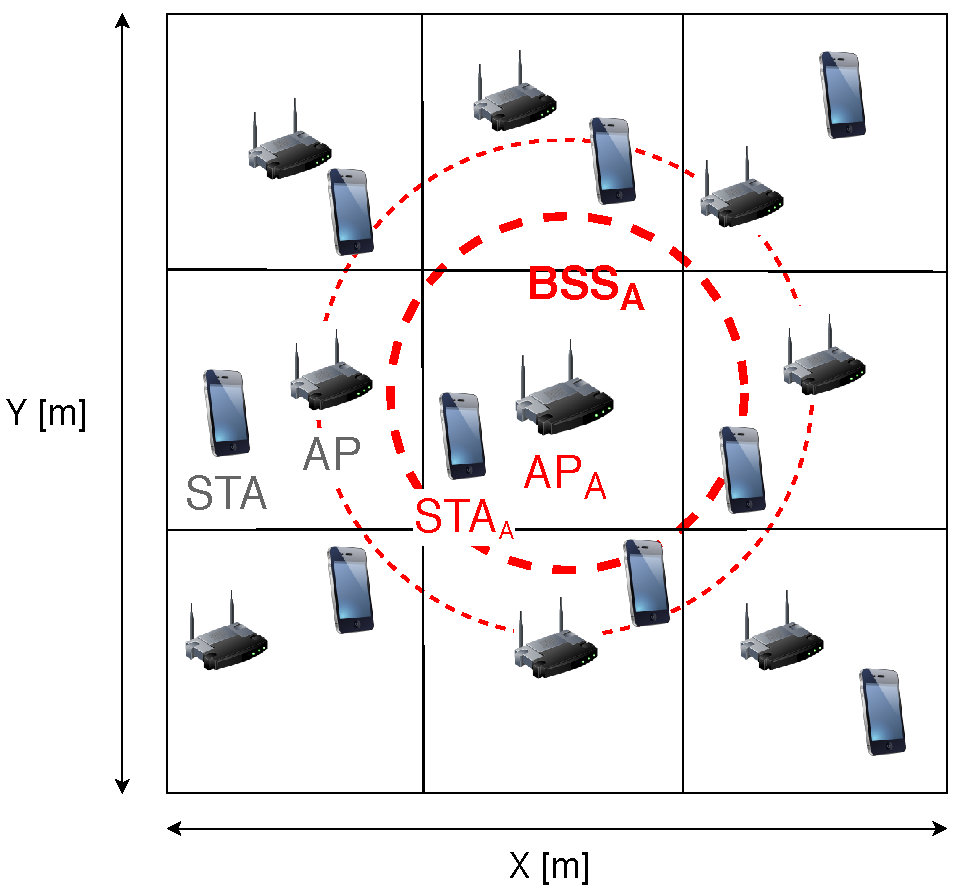
\epsfig{file=random_scenario.pdf, width=5.5cm}
	\caption{Random grid scenario containing 9 BSSs. The location of $\text{BSS}_\text{A}$ is fixed at the center for the sake of analysis.}
	\label{fig:random_scenario}
\end{figure}

The simulation parameters are provided in Table \ref{table:parameters}.\footnote{\textcolor{black}{For more details on the Komondor's packet reception and interference models, we refer the interested reader to \cite{barrachina2019komondor}.}} The scenario is divided into nine cells, but the location of $\text{BSS}_\text{A}$ is always fixed at the center of the scenario for the sake of analysis. For the rest of the APs and STAs, their position is randomly selected within their corresponding cell. The configuration of each BSS is set homogeneously, i.e., they all use the same channel, the default sensitivity is set to -82 dBm, and the default transmission power is set to 20 dBm. Notice that, for dense deployments, $\text{BSS}_\text{A}$ is expected to suffer a higher level of interference than the others, which allows us to assess the effectiveness of the SR operation in crowded environments.

\begin{table}[h]
	\centering
	\resizebox{.6\columnwidth}{!}{
		\begin{tabular}{c|l|l|}
			\cline{2-3}
			\multicolumn{1}{l|}{} & \textbf{Parameter} & \textbf{Value}
			\\ \hline
			% PHY
			\multicolumn{1}{|c|}{\multirow{9}{*}{\rotatebox[origin=c]{90}{PHY}}} & Central frequency, $f_c$ & 5 GHz \\ \cline{2-3} 
			\multicolumn{1}{|c|}{} & Transmission gain, $G_{tx}$ & 0 dB \\ \cline{2-3} 
			\multicolumn{1}{|c|}{} & Reception gain, $G_{rx}$ & 0 dB \\ \cline{2-3} 
			\multicolumn{1}{|c|}{} & Path-loss (residential scenario), $\text{PL}(d)$ & See (\cite{pathloss11ax})  \\ \cline{2-3}
			\multicolumn{1}{|c|}{} & Background noise level, $N$ & -95 dBm \\ \cline{2-3}
			\multicolumn{1}{|c|}{} & Legacy OFDM symbol duration, $\sigma_\text{leg}$ & 4 \textmu s \\
			\cline{2-3}
			\multicolumn{1}{|c|}{} & OFDM symbol duration (GI-32), $\sigma$ & 16 \textmu s \\ 				\cline{2-3}
			\multicolumn{1}{|c|}{} & Number of subcarriers (20 MHz), $N_{sc}$ & 234   \\
			\cline{2-3}
			\multicolumn{1}{|c|}{} & Number of spatial streams, $N_{ss}$ & 1  \\
			\cline{2-3}
			\multicolumn{1}{|c|}{} & Transmit power levels, $\mathcal{T}$ & 1 to 20 dBm (1 dBm steps) \\
			\hline
			% MAC
			\multicolumn{1}{|c|}{\multirow{16}{*}{\rotatebox[origin=c]{90}{MAC}}} & Empty slot duration, $\text{T}_e$ & 9 $\mu$s\\ 
			\cline{2-3} 
			\multicolumn{1}{|c|}{} & SIFS duration, $T_\text{SIFS}$ & 16 \textmu s  \\
			\cline{2-3} 
			\multicolumn{1}{|c|}{} & DIFS/AIFS duration, $T_\text{DIFS/AIFS}$ & 34 \textmu s \\
			\cline{2-3} 
			\multicolumn{1}{|c|}{} & PIFS duration, $T_\text{PIFS}$  & 25 \textmu s \\
			\cline{2-3} 
			\multicolumn{1}{|c|}{} & Legacy preamble duration, $T_\text{PHY-leg}$ & 20 \textmu s  \\
			\cline{2-3}
			\multicolumn{1}{|c|}{} & HE single-user field duration, $T_\text{HE-SU}$ & 100 \textmu s \\
			\cline{2-3} 
			\multicolumn{1}{|c|}{} & ACK duration, $T_\text{ACK}$ & 28 \textmu s\\
			\cline{2-3} 
			\multicolumn{1}{|c|}{} & Block ACK duration, $T_\text{BACK}$ & 32 \textmu s \\
			\cline{2-3} 
			\multicolumn{1}{|c|}{} &  Size OFDM symbol (legacy), $L_{s,l}$ & 24 bits \\
			\cline{2-3} 
			\multicolumn{1}{|c|}{} & Length of data packets, $\text{L}_{d}$ & 12,000 bits \\
			\cline{2-3} 
			\multicolumn{1}{|c|}{} & No. of frames in an A-MPDU, $N_{\text{agg}}$ & 64 \\
			\cline{2-3} 
			\multicolumn{1}{|c|}{} & Length of an RTS packet, $L_\text{RTS}$ & 160 bits \\
			\cline{2-3} 
			\multicolumn{1}{|c|}{} & Length of a CTS packet, $L_\text{CTS}$ & 112 bits \\
			\cline{2-3} 
			\multicolumn{1}{|c|}{} & Length of service field, $L_\text{SF}$ & 16 bits  \\
			\cline{2-3} 
			\multicolumn{1}{|c|}{} & Length of MAC header, $L_\text{MH}$ & 320 bits \\
			\cline{2-3} 
			\multicolumn{1}{|c|}{} & Contention window (fixed), $\text{CW}$ & 15 \\
			\cline{2-3} 
			\multicolumn{1}{|c|}{} & Allowed sensitivity levels, $\mathcal{S}$ & -82 to -62 (1 dBm steps) \\
			\hline
			% Other
			\multicolumn{1}{|c|}{\multirow{2}{*}{\centering\rotatebox[origin=c]{90}{Misc.  }}} & Traffic model, $\Lambda$ & Downlink (UDP)\\
			\cline{2-3} 
			\multicolumn{1}{|c|}{} & Traffic generation ratio, $l$ & 1,000, 2,000, 10,000 pkts/s\\ 
			\cline{2-3} 
			\multicolumn{1}{|c|}{} & Map area (random scenario), $A$ & 625, 400, 225, 100 m$^2$\\
			\hline
	\end{tabular}}
	\caption{Simulation parameters.}
	\label{table:parameters}
\end{table}

%%% DENSITY
\subsection{Network Density}
\label{section:random_scenarios_density}
To analyze SR based on the network density, we consider four different map sizes: sparse ($25\times25$ m), semi-dense ($20\times20$ m), dense ($15\times15$ m) and ultra-dense ($10\times10$ m). For each type of scenario, we provide 50 different deployments, in which APs and STAs are placed uniformly at random within their corresponding cell. $\text{BSS}_\text{A}$ is the only one applying the SR operation. Since we compute all the possible OBSS/PD values to be used by $\text{BSS}_\text{A}$, each random deployment leads to $21\times4\times50$ = 4,200 different scenarios.

Fig.~\ref{fig:SIM_2_1} shows the average throughput achieved under the default and the SR settings\textcolor{black}{, respectively}. In particular, we differentiate between the individual throughput of $\text{BSS}_\text{A}$ and the average throughput of the other BSSs. For each network density, we have tried all the possible OBSS/PD values and compared the best one to the default CCA/CS.

\begin{figure}[ht!]
	\centering		
	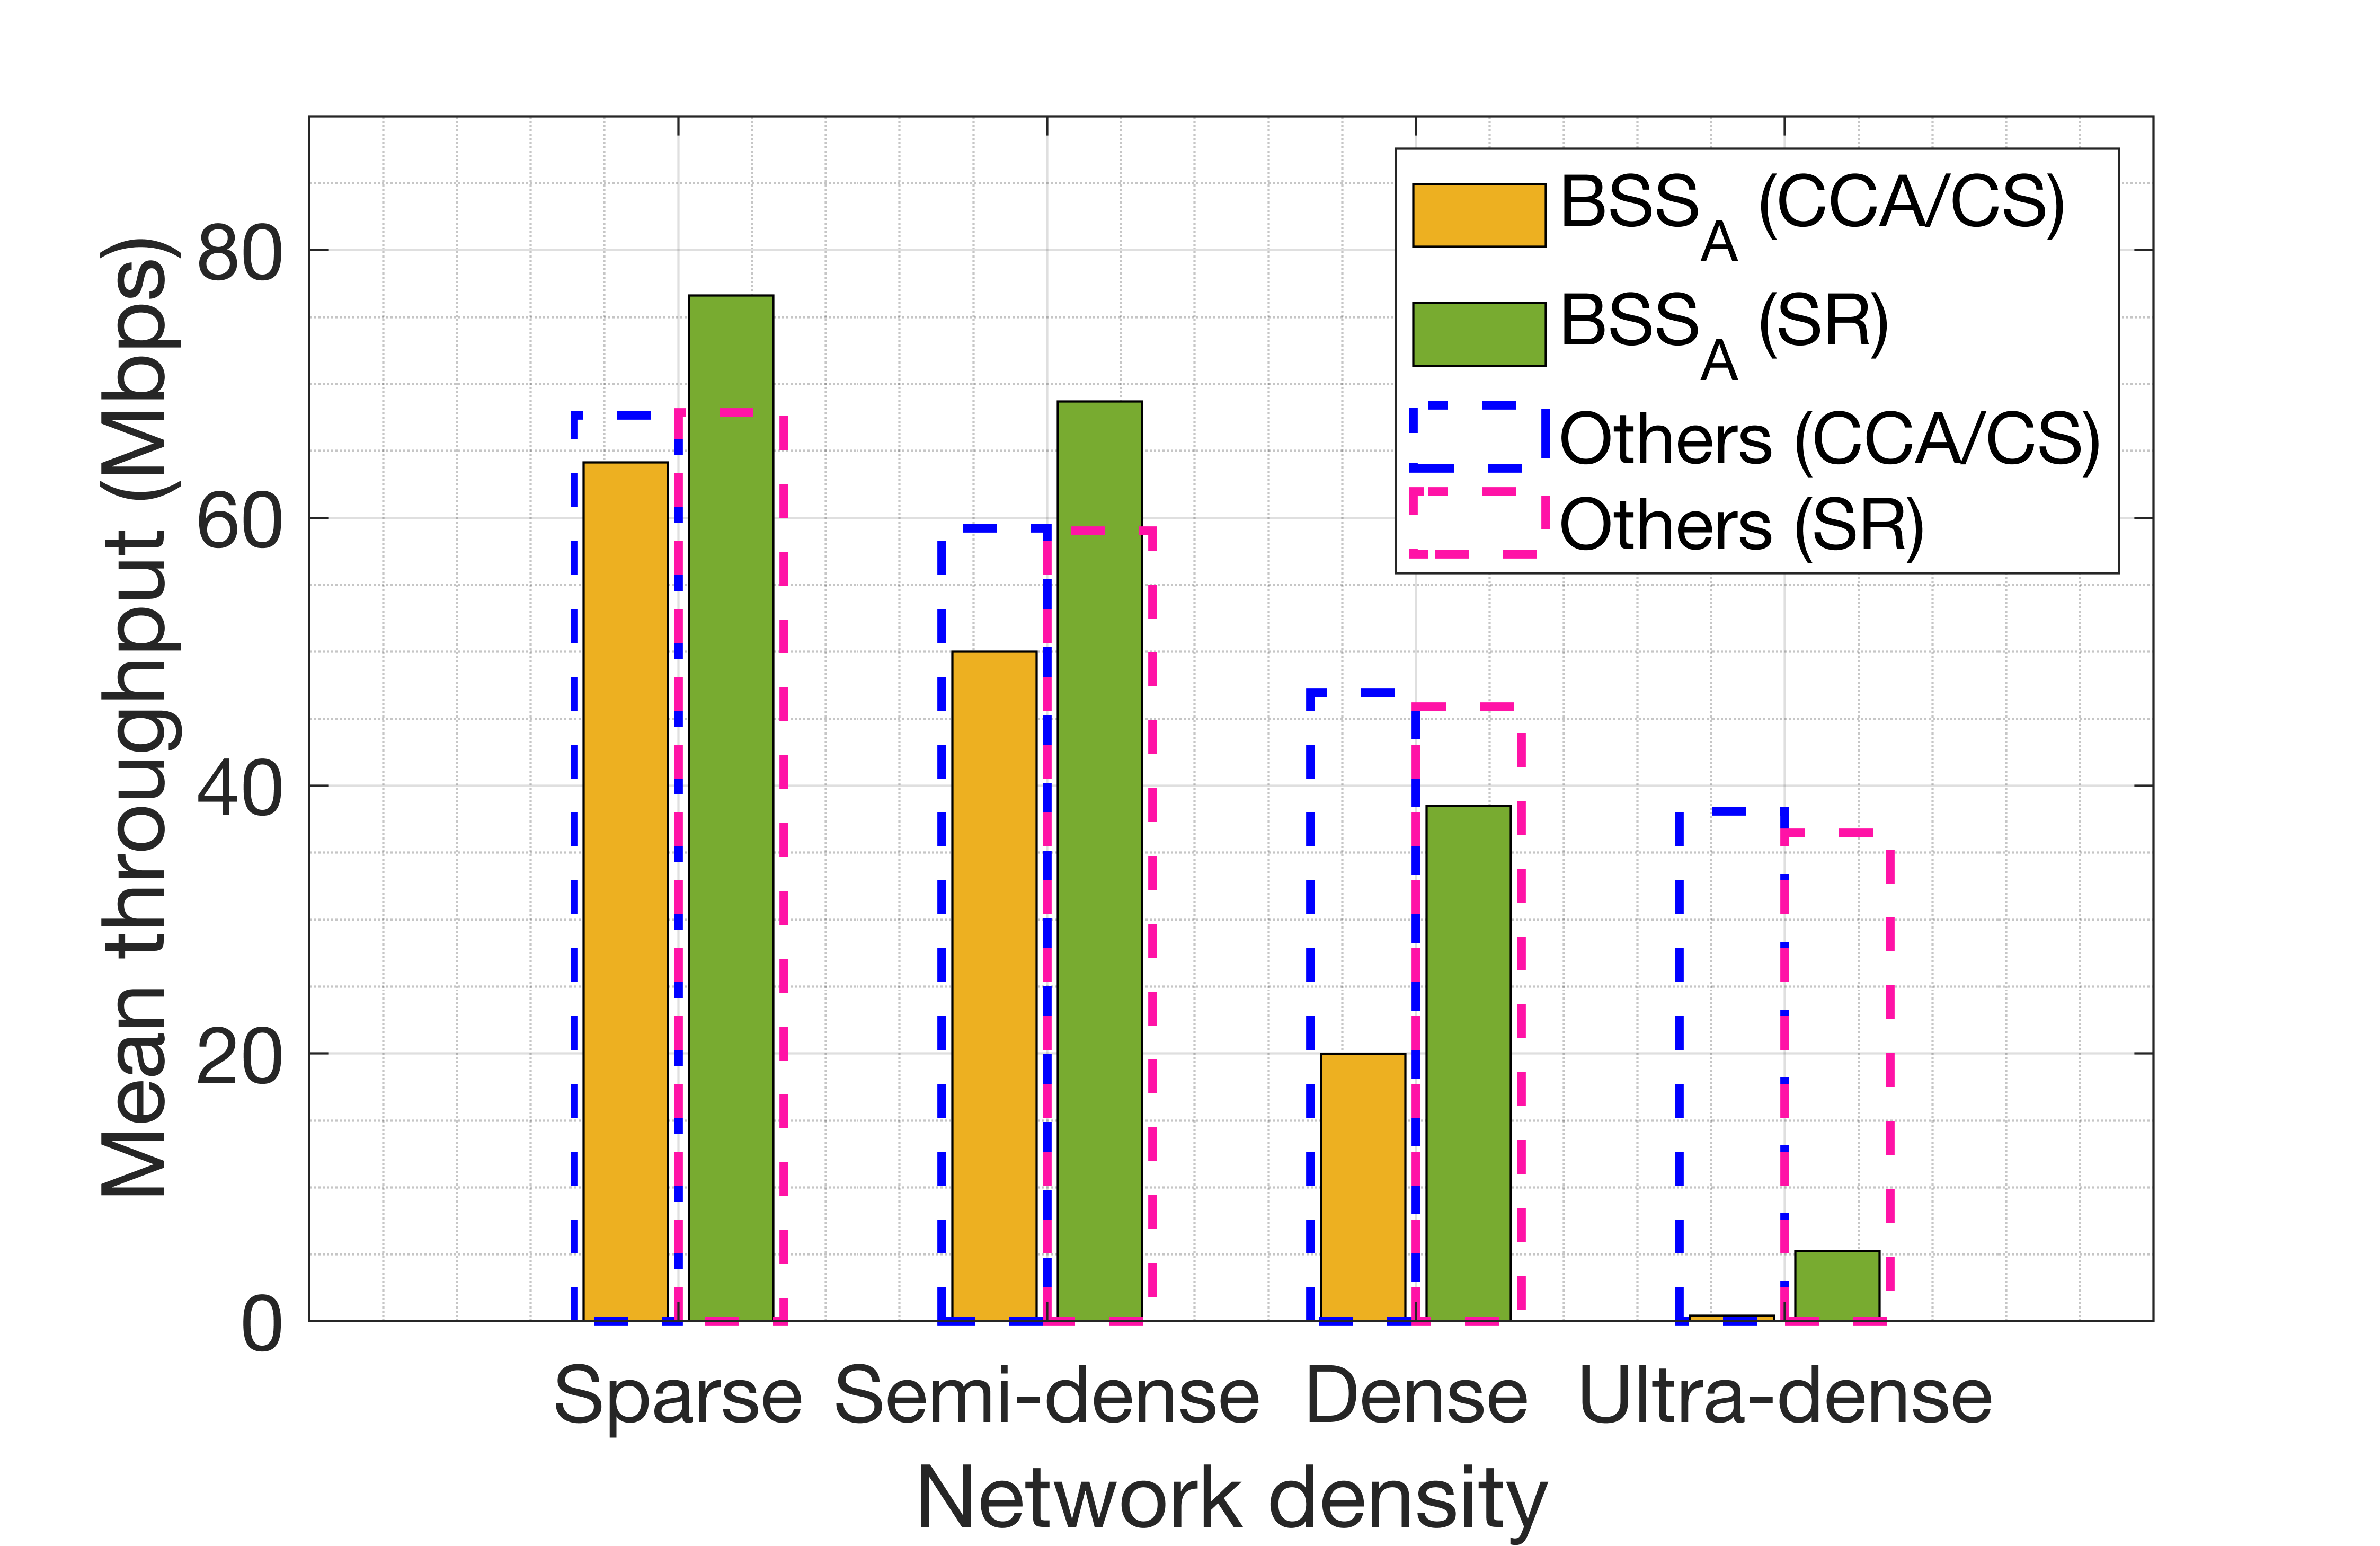
\includegraphics[width=.48\columnwidth]{SIM_2_1}
	\caption{Mean throughput achieved with and without applying the SR operation in $\text{BSS}_\text{A}$, for each network density. Results show the mean throughput achieved by $\text{BSS}_\text{A}$ and the rest of BSSs.}
	\label{fig:SIM_2_1}
\end{figure}

First of all, we focus on the throughput that $\text{BSS}_\text{A}$ experiences by default (\textcolor{black}{solid amber} bars). We notice a dramatic decrease as network density increases. Nevertheless, the SR operation allows $\text{BSS}_\text{A}$ to significantly improve the throughput (displayed by the \textcolor{black}{solid green} bars). Note, as well, that the maximum improvement is experienced at the dense scenario ($15\times15$ m). While the default performance is quite high for sparser scenarios, channel re-utilization cannot be significantly improved at the ultra-dense scenario due to the high level of inter-BSS interference.

Apart from that, we observe that the average performance of the other BSSs (dashed bars) does not suffer radical changes for any of the network densities when $\text{BSS}_\text{A}$ applies SR. This is a really positive result, which indicates that SR allows improving the individual performance without affecting the rest of \textcolor{black}{the} devices that do not apply the operation.

%%% TRAFFIC LOAD
\subsection{Traffic load}
\label{section:random_scenarios_traffic_load}
\textcolor{black}{Besides network density, we now analyze the impact of the traffic load on the SR operation.} To that purpose, we focus on the second densest scenario, which has been previously shown to achieve the maximum gains of the SR operation. In particular, we provide three different traffic loads ($l$), which are the same for all the BSSs: \emph{i)} low (1,000 packets/s, i.e., 12 Mbps), \emph{ii)} medium (2,000 packets/s, i.e., 24 Mbps), and \emph{iii)} high (10,000 packets/s, i.e., 120 Mbps). The traffic type considered is UDP in the downlink, which follows a Poisson distribution with $\lambda$ \textcolor{black}{equals to the traffic load.}

Fig.~\ref{fig:SIM_2_2} compares the performance achieved by default and SR configurations, for the different proposed traffic load values. As done before, the results show the individual performance of $\text{BSS}_\text{A}$ and the average performance of the rest of BSSs. In particular, Fig.~\ref{fig:SIM_2_2_2} shows the maximum improvements achieved by BSS$_\text{A}$ in terms of throughput. Notice that the SR configuration considers the OBSS/PD values that maximize BSS$_\text{A}$'s throughput. Based on that configuration, Fig.~\ref{fig:SIM_2_2_1} shows the average channel occupancy (in \%).

\begin{figure}[ht!]
	\centering		
	%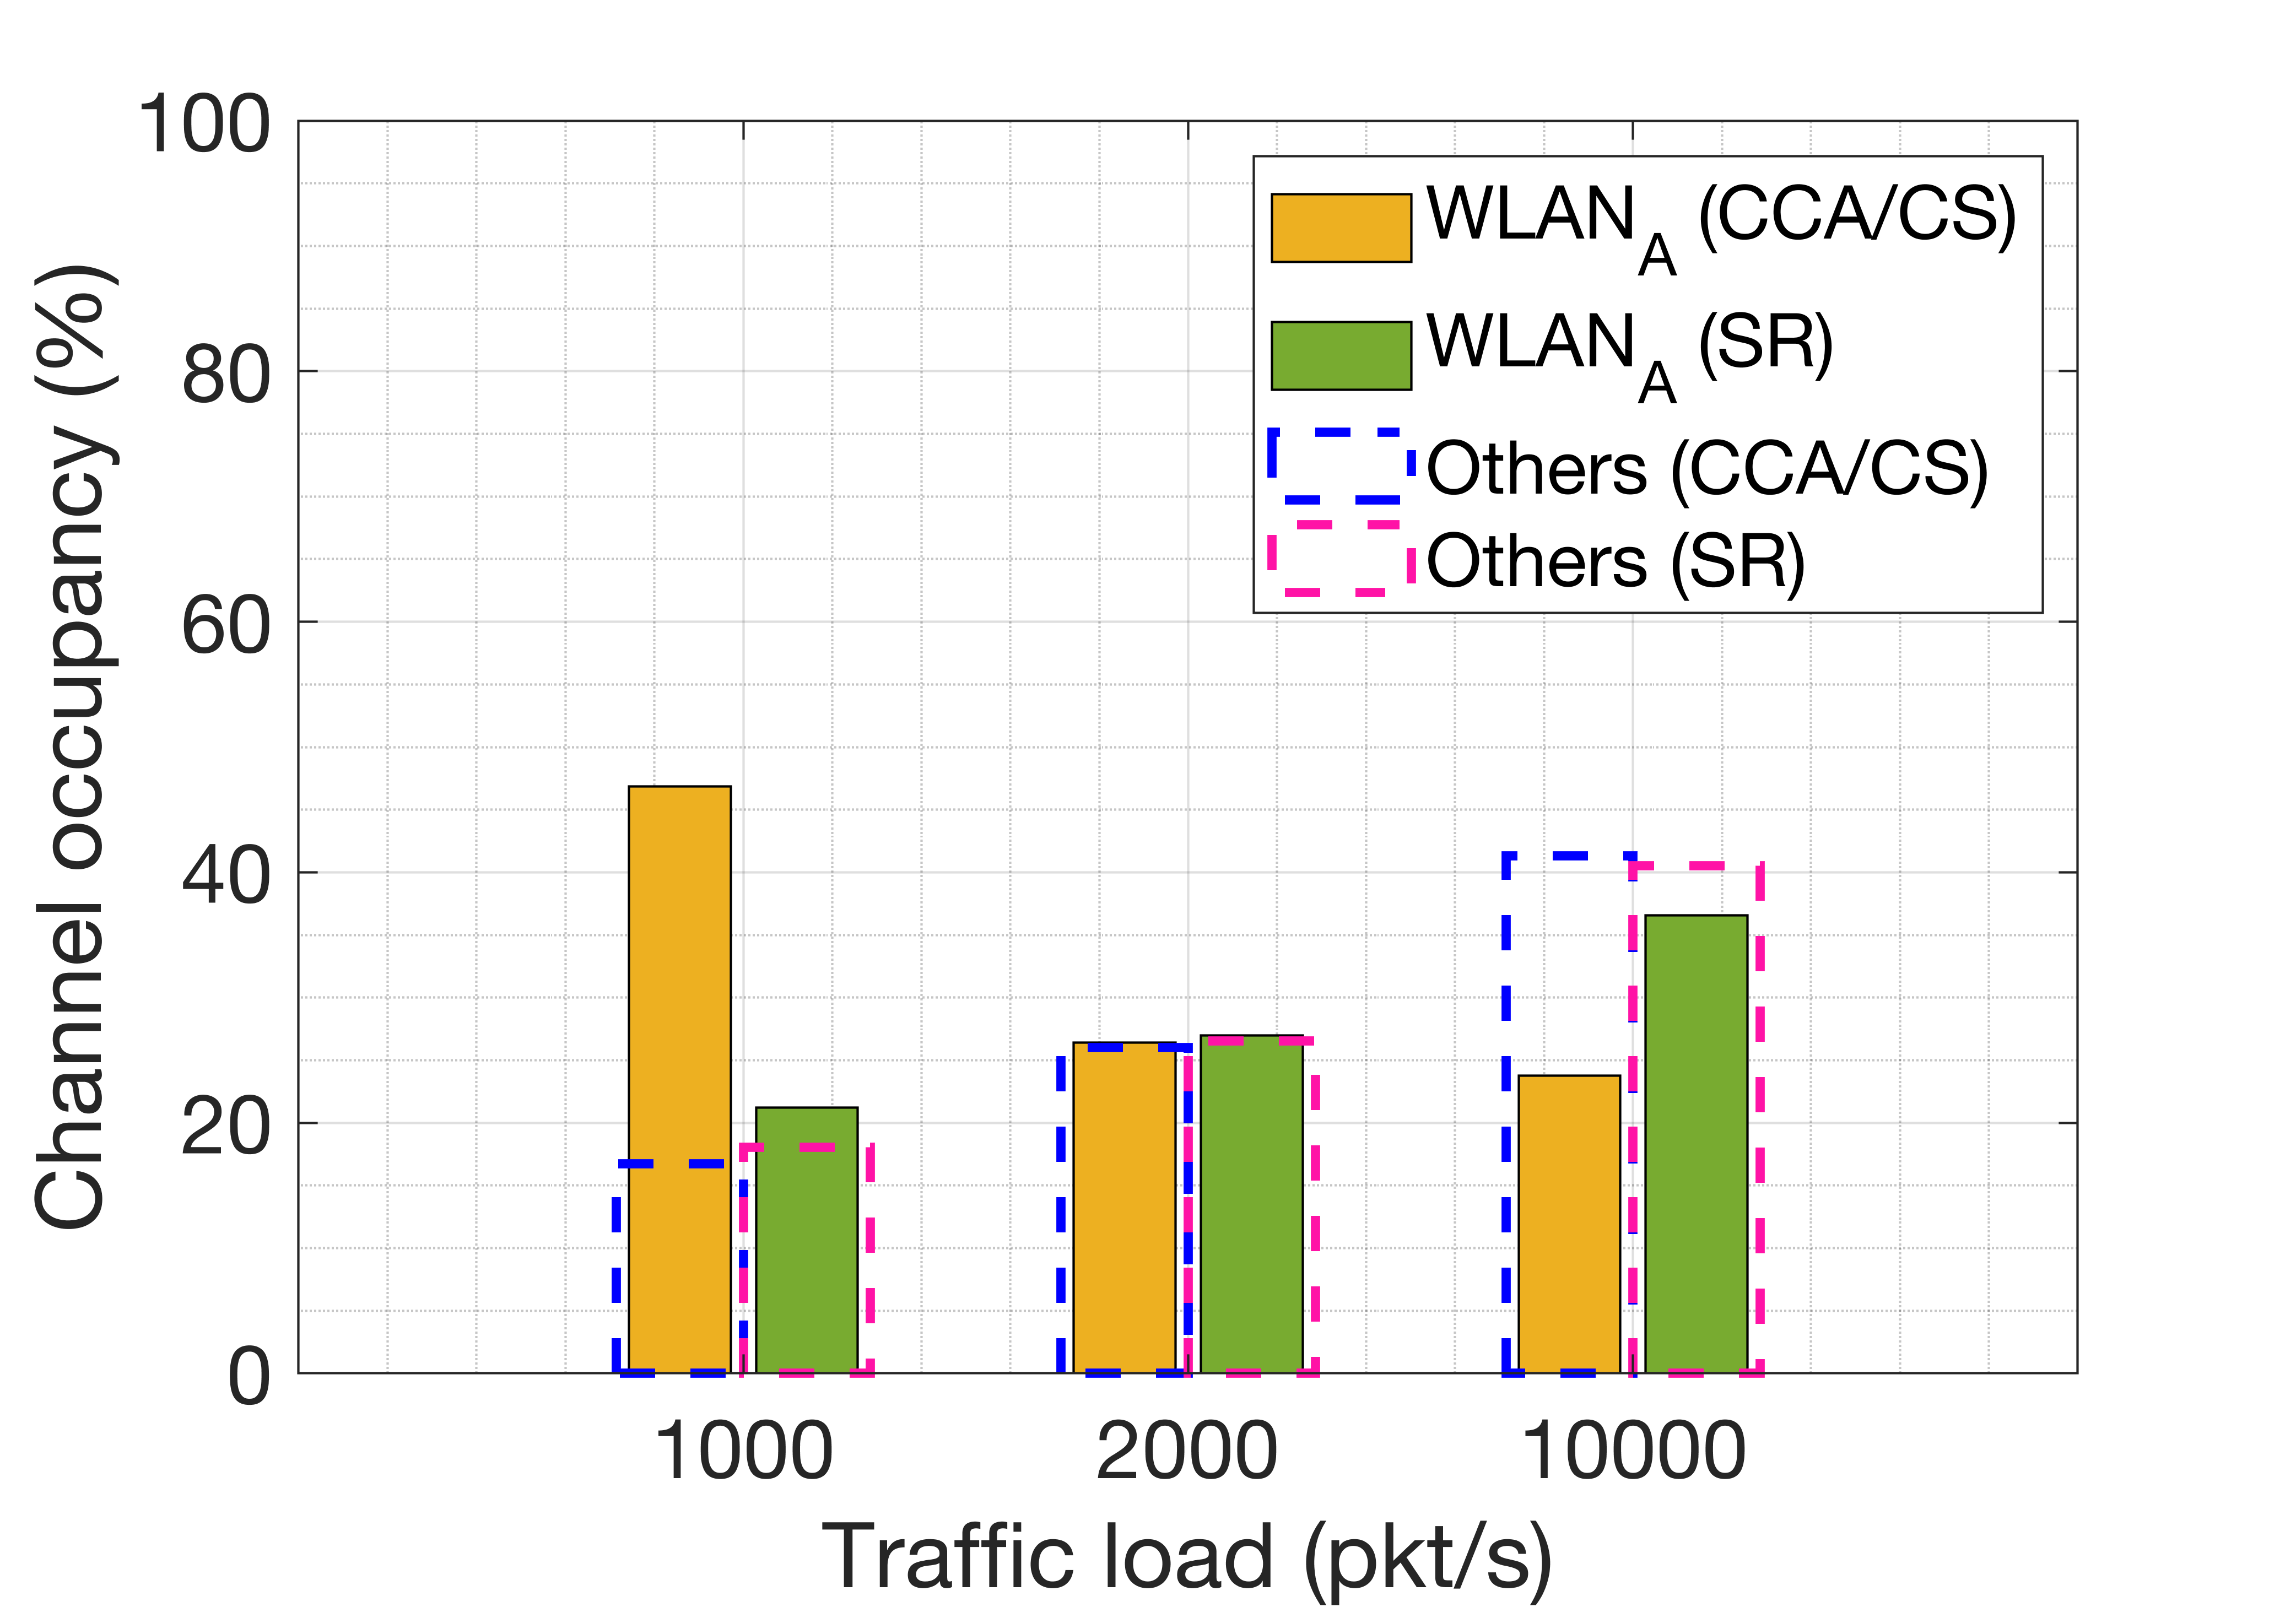
\includegraphics[width=\columnwidth]{SIM_2_2_1}
	\subfigure[Throughput]{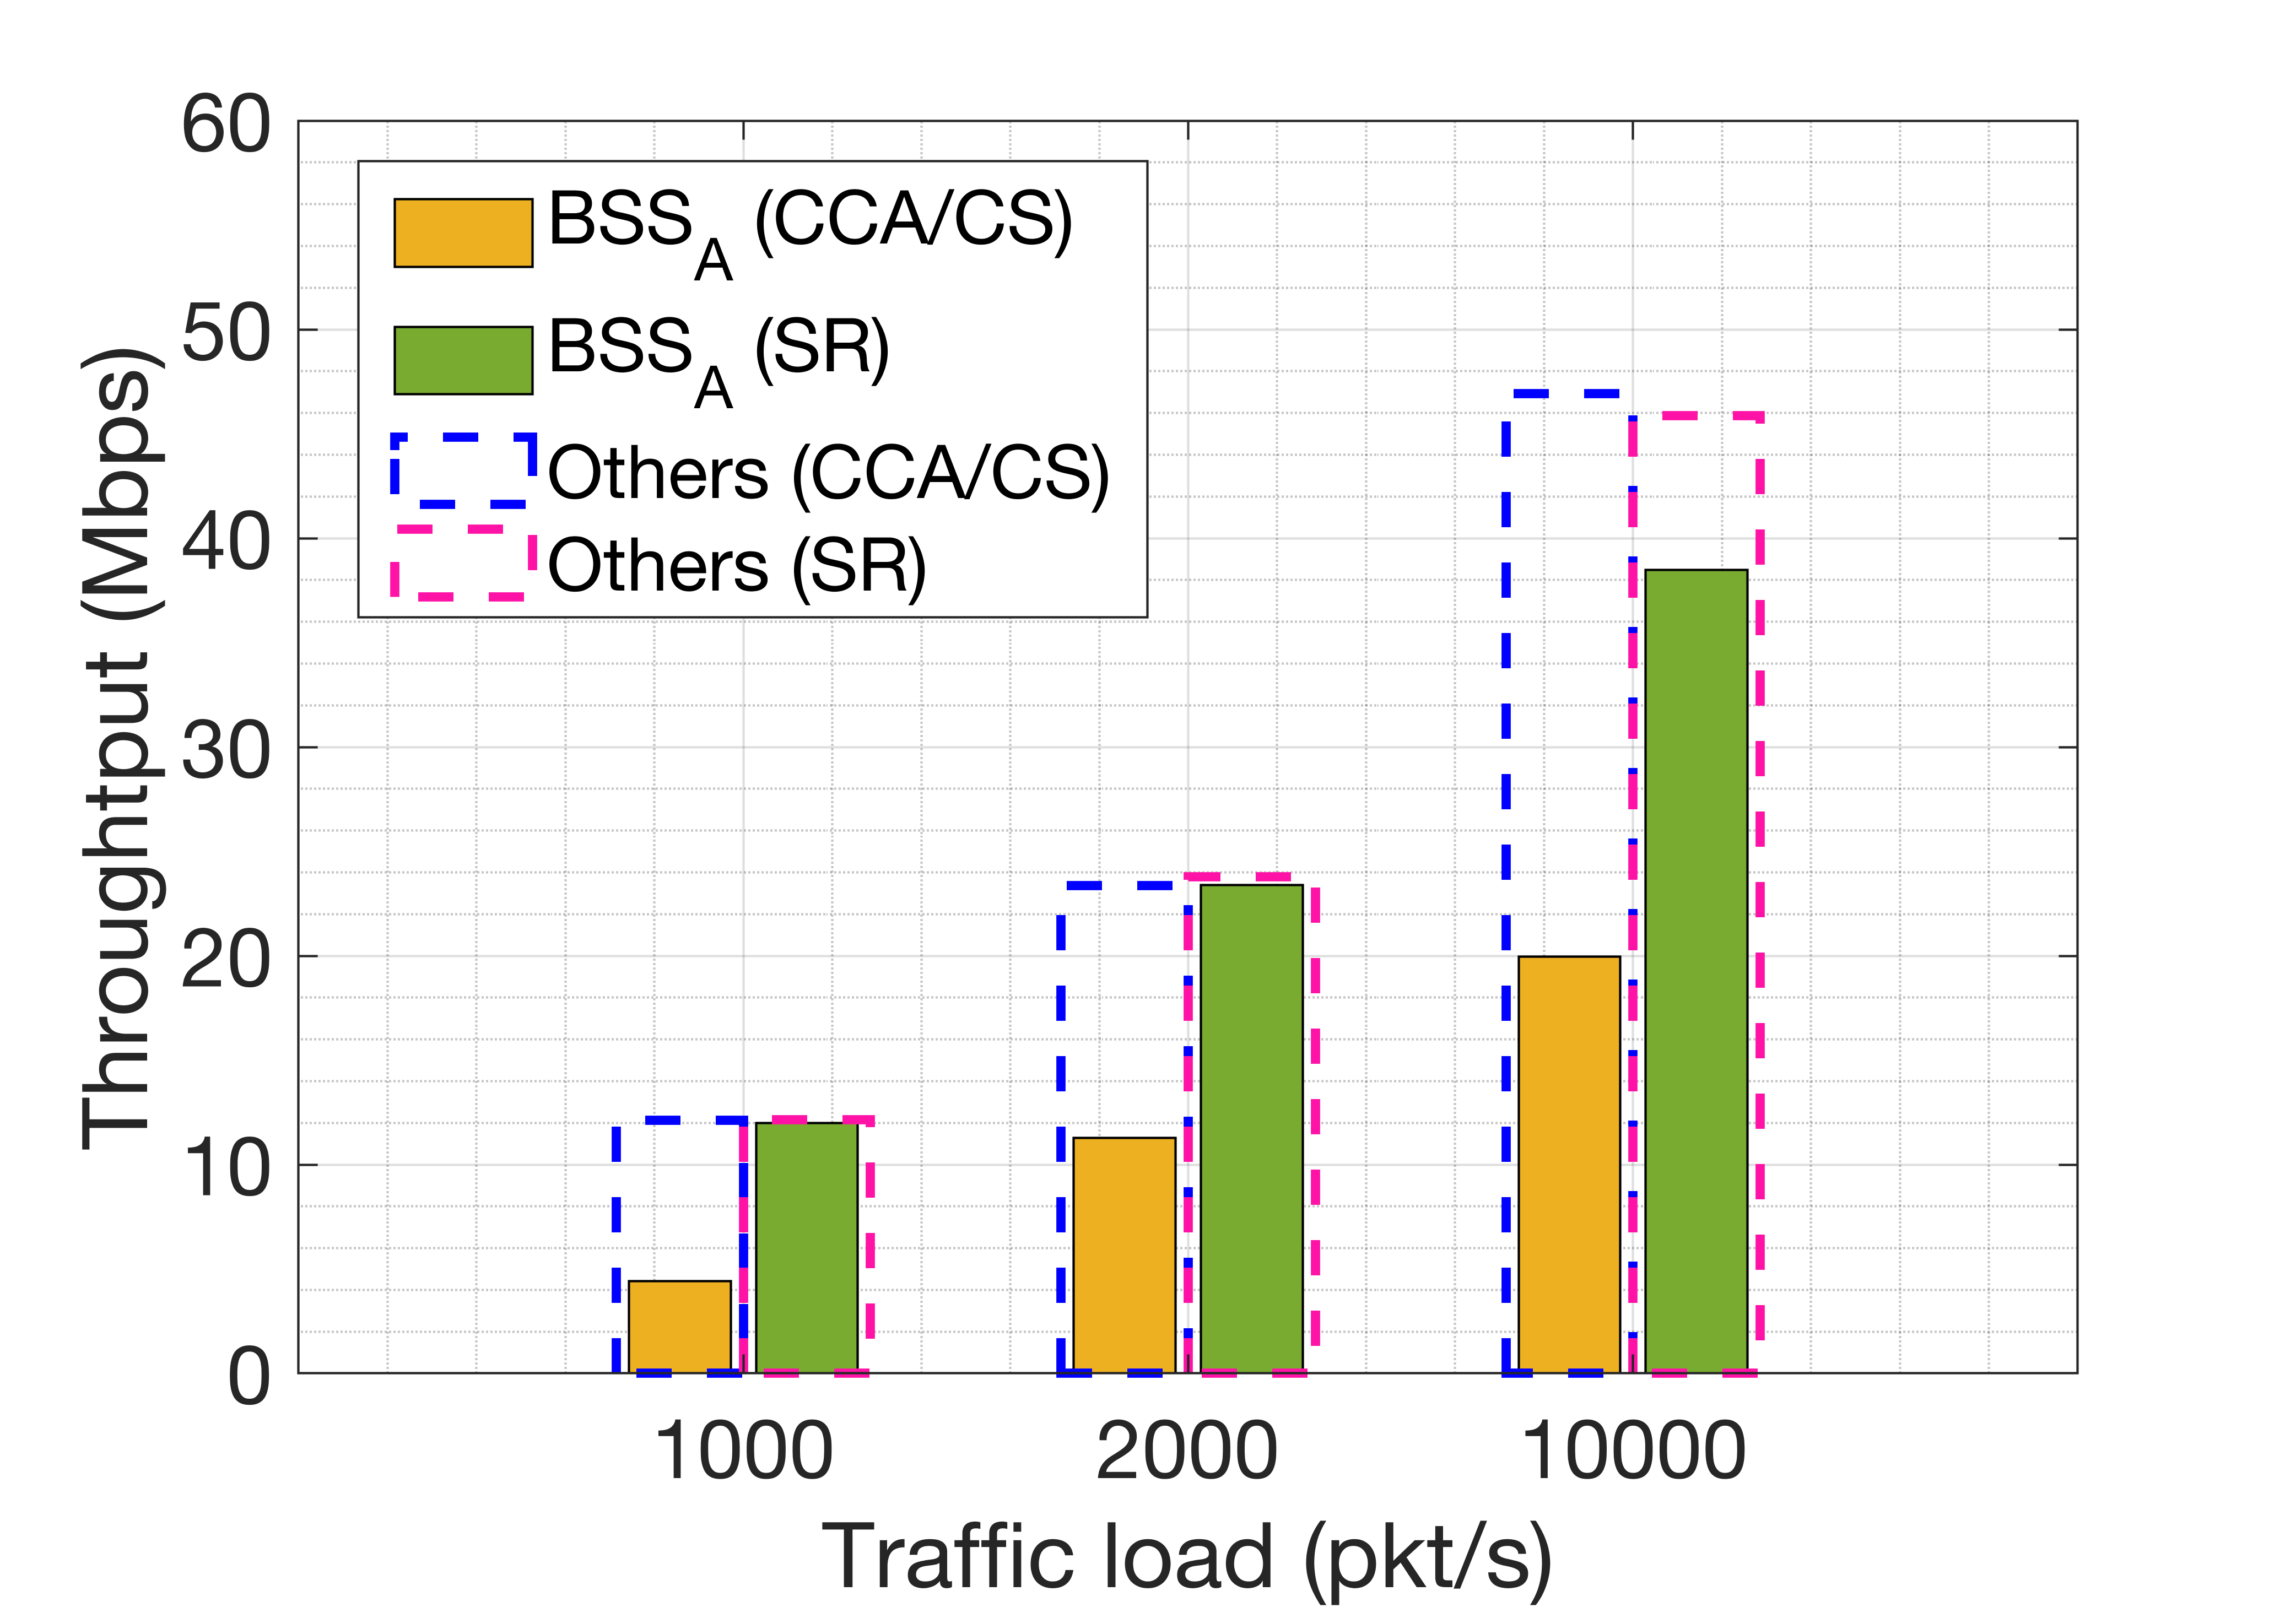
\includegraphics[width=.48\columnwidth]{SIM_2_2_2}\label{fig:SIM_2_2_2}}
	\subfigure[Channel occupancy]{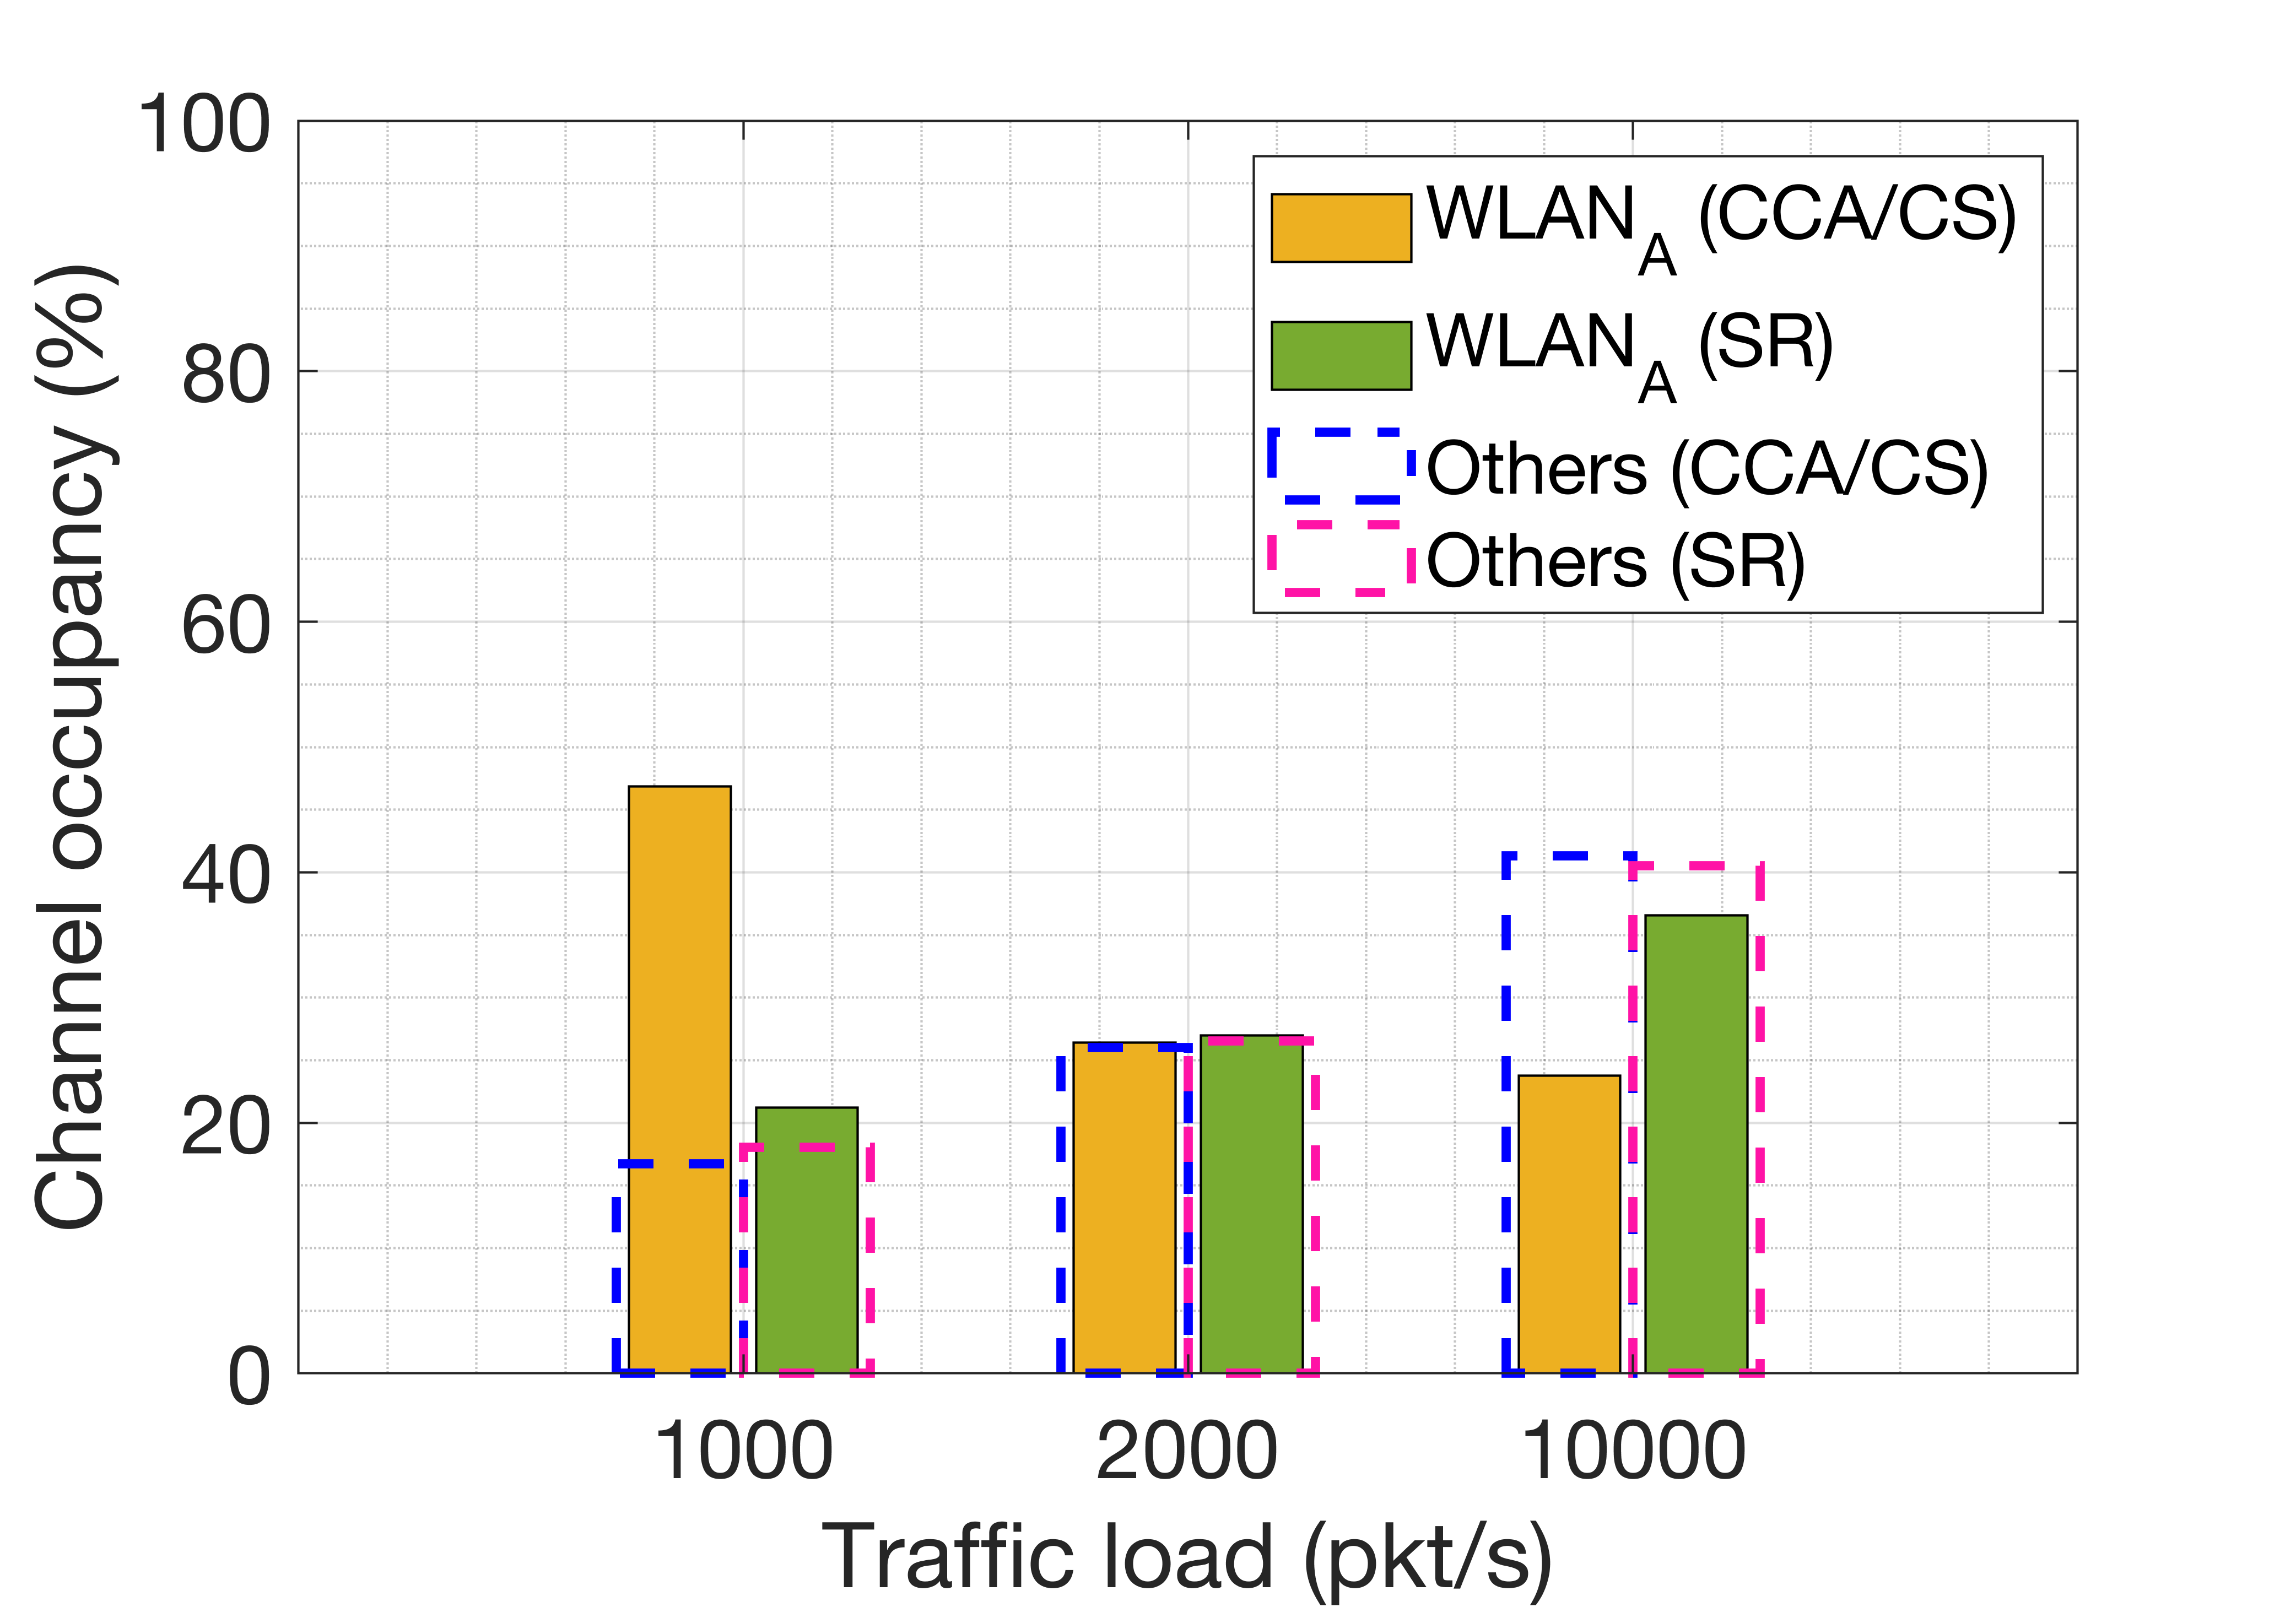
\includegraphics[width=.48\columnwidth]{SIM_2_2_1}\label{fig:SIM_2_2_1}}
	\caption{Mean throughput and channel occupancy achieved with and without applying the SR operation in $\text{BSS}_\text{A}$, for each traffic load. Results are shown for $\text{BSS}_\text{A}$ and for the rest of BSSs (others).}
	\label{fig:SIM_2_2}
\end{figure}

As shown in Fig.~\ref{fig:SIM_2_2_2}, $\text{BSS}_\text{A}$ obtains higher throughput gains as the traffic load increases. In particular, the highest gain is noticed for the largest traffic load (10,000 packets/s), which entails a saturation regime. This is \textcolor{black}{quite a} remarkable result since the interference noticed by $\text{BSS}_\text{A}$ is much higher when all the surrounding devices are constantly transmitting due to their high traffic load. \textcolor{black}{Note, as well, that we are considering a dense scenario, which entails that the probability for BSS$_\text{A}$ to sense the channel busy is significantly high even for the lowest traffic load.} Regarding channel occupation (shown in Fig.~\ref{fig:SIM_2_2_1}), an interesting phenomenon is observed for the lowest traffic load. The fact is that the legacy CCA/CS configuration provides a higher channel occupancy than the SR one. However, this is not translated into higher throughput due to the high number of experienced collisions. Notice that collisions entail a high number of re-transmissions, which cause the observed increase in the occupancy. Finally, it is worth pointing out that the performance of the other BSSs is not affected when $\text{BSS}_\text{A}$ applies SR.

%%% COLLABORATIVE SR
\subsection{Joint Spatial Reuse Operation}
\label{section:random_scenarios_collaborative}

\begin{figure*}[ht!]
	\centering		
	\subfigure[BSS$_\text{A}$]{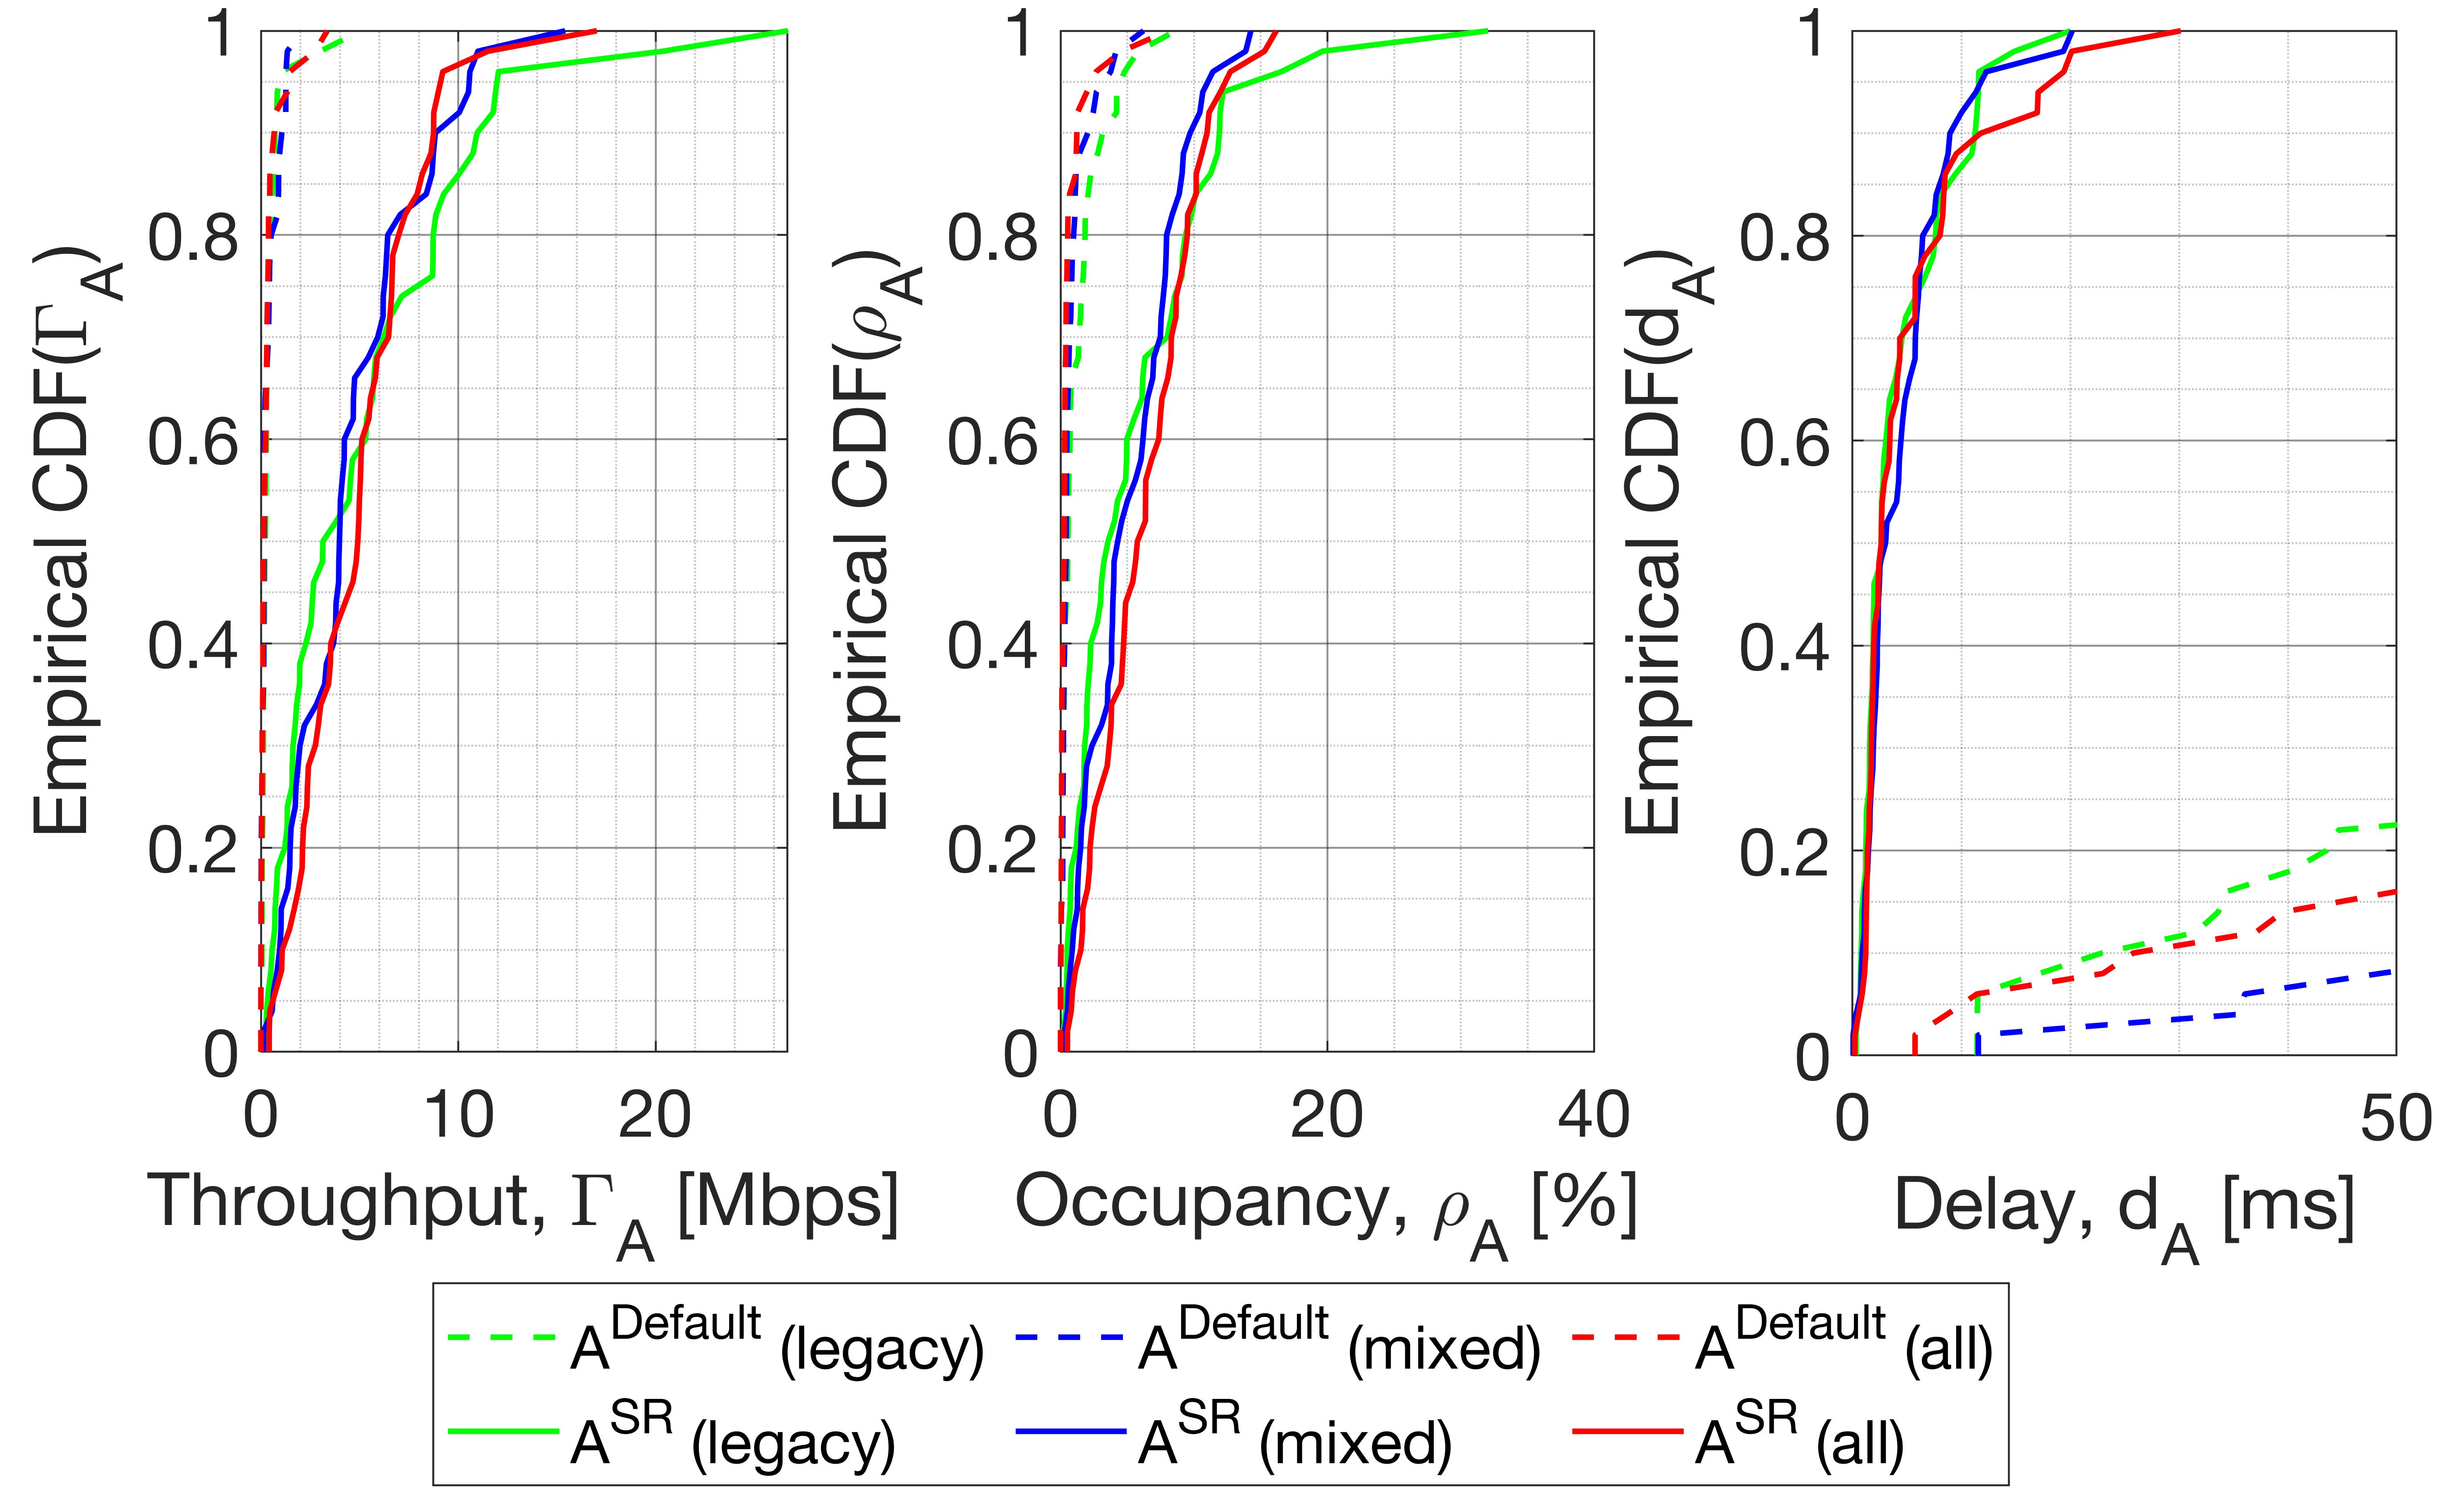
\includegraphics[width=.52\columnwidth]{SIM_2_3_1}\label{fig:SIM_2_3_1}}%
	\subfigure[Others]{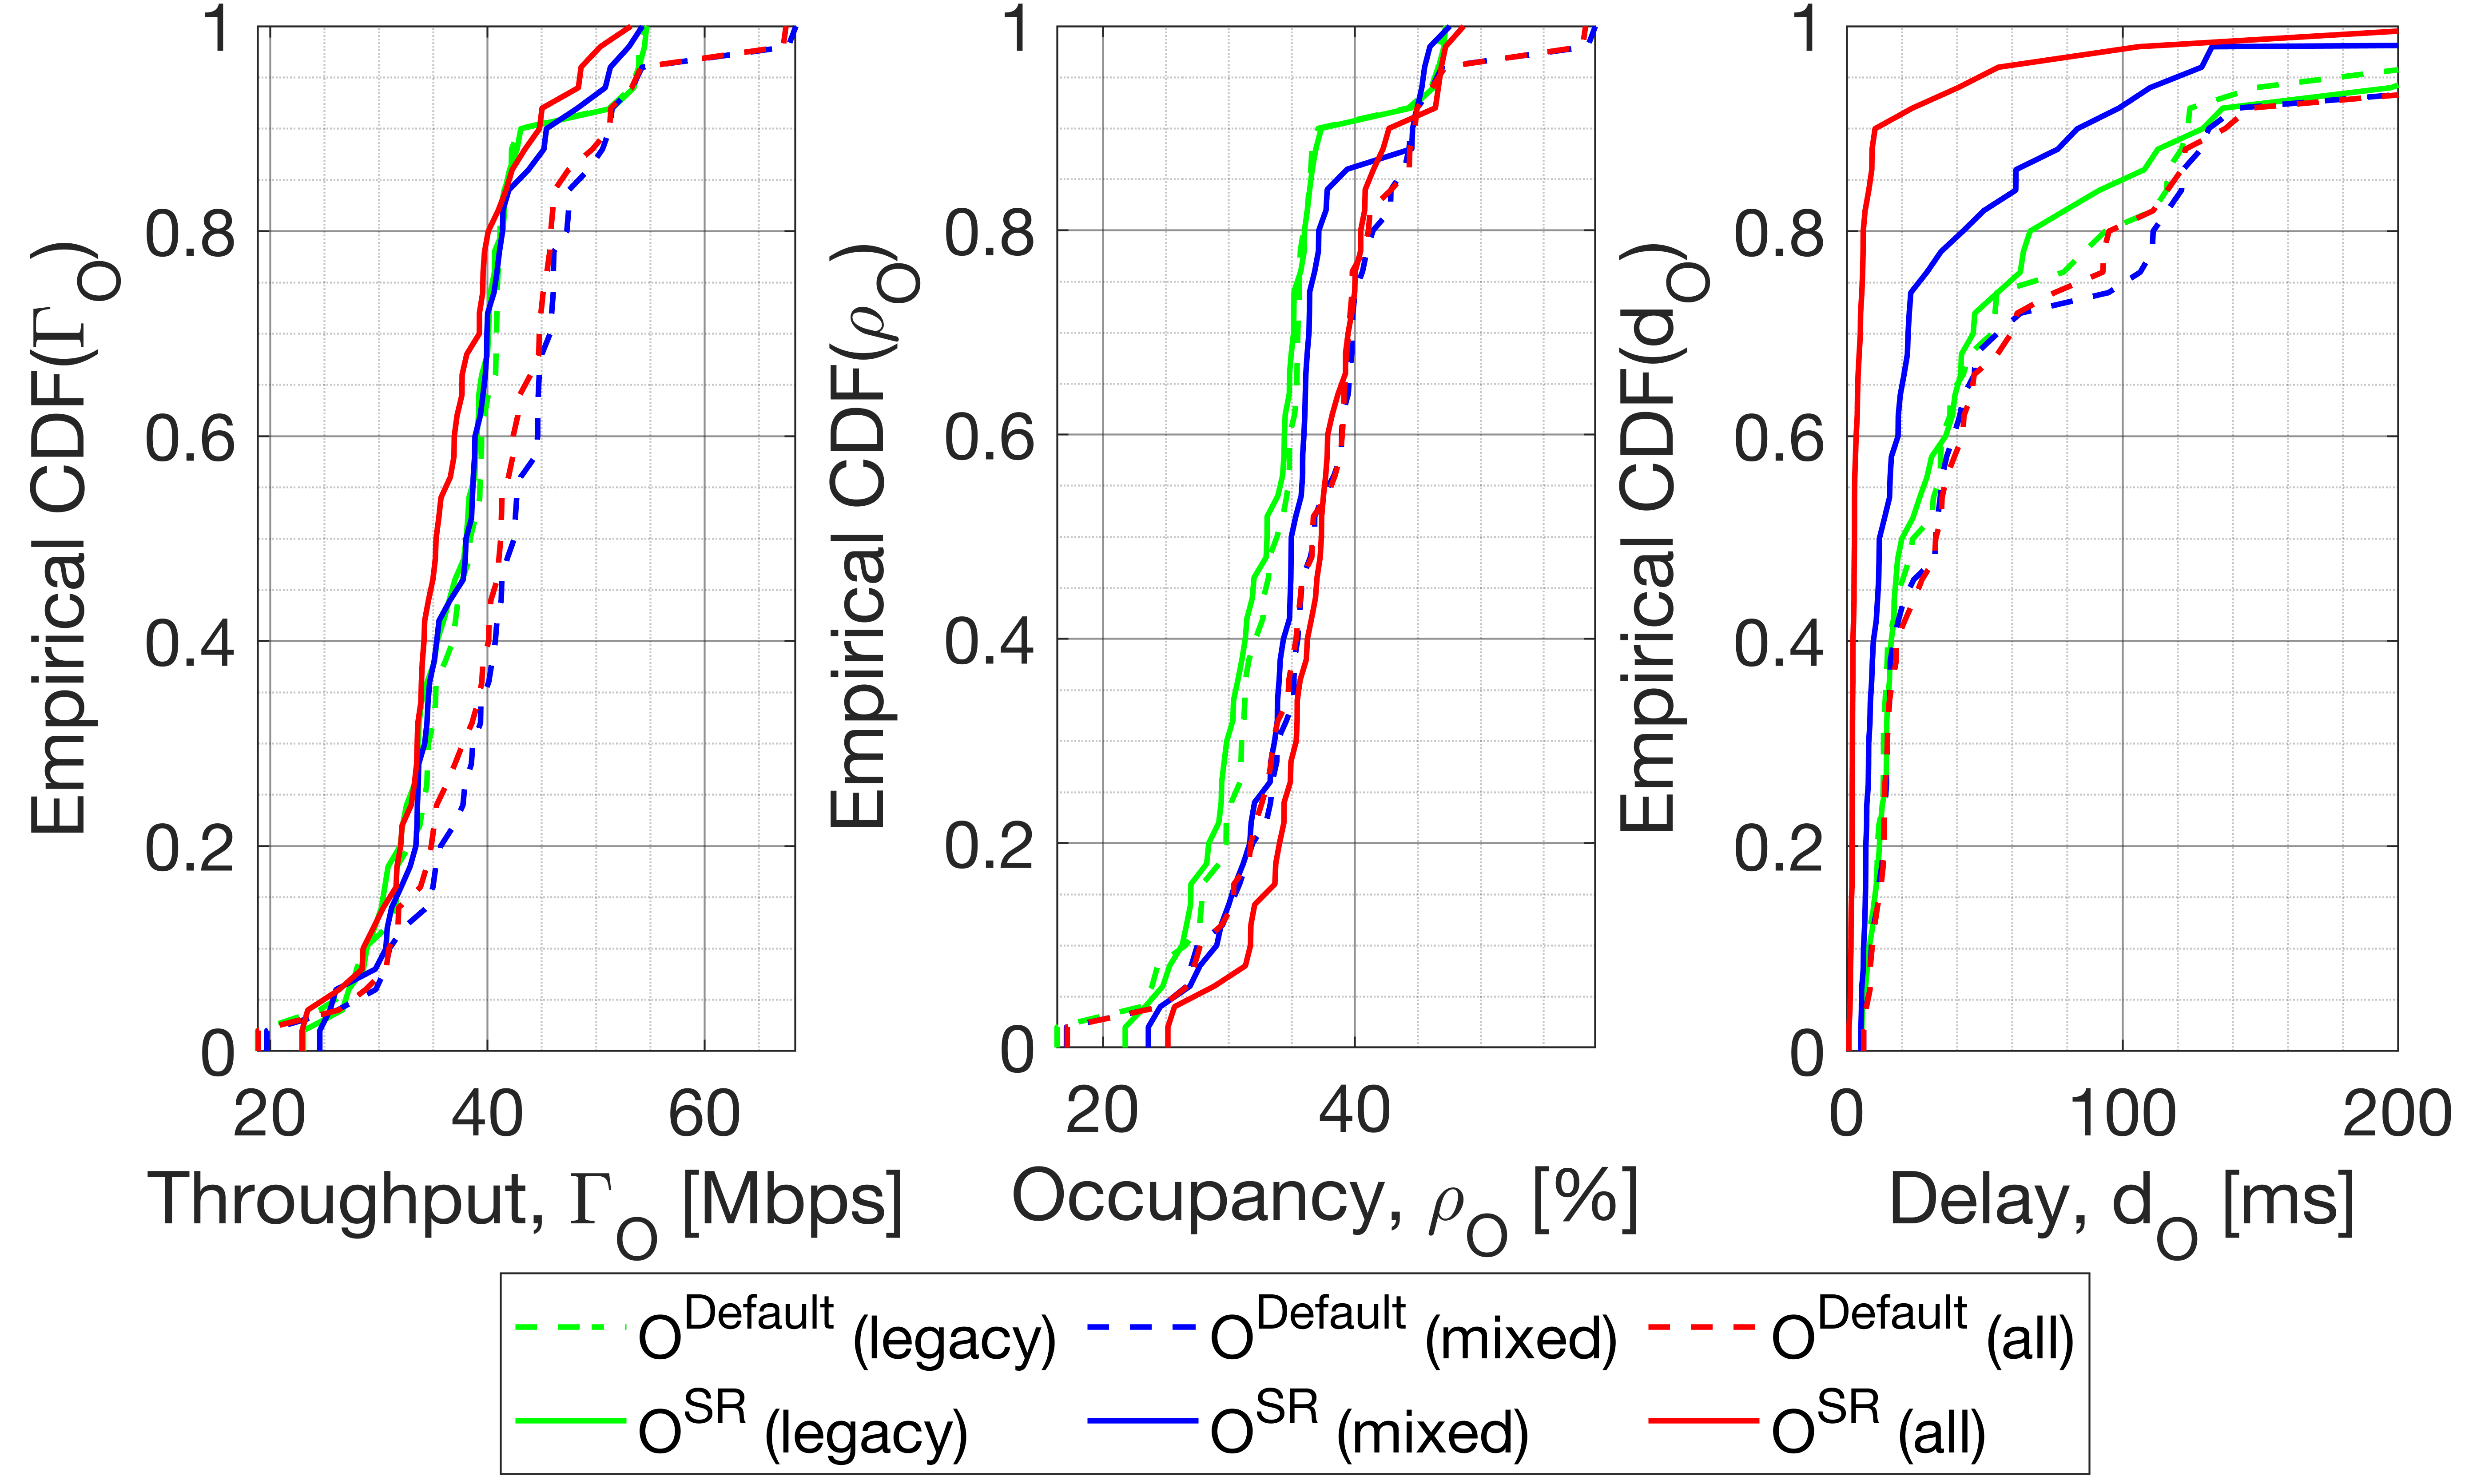
\includegraphics[width=.52\columnwidth]{SIM_2_3_2}\label{fig:SIM_2_3_2}}
	\caption{Mean performance improvements achieved for each SR setting by BSS$_\text{A}$ ($A$) and the others ($O$). The results are shown for the OBSS/PD values that maximize the performance of BSS$_\text{A}$.}\label{fig:SIM_2_3}
\end{figure*}

So far, we have studied the effects of applying SR at a single BSS (i.e., $\text{BSS}_\text{A}$). \textcolor{black}{Now, we focus on the concurrent behavior of the SR operation. Provided that $\text{BSS}_\text{A}$ always applies SR, we propose three study cases according to the set of neighbors that also apply it: }
\begin{itemize}
	\item \textbf{Legacy:} all the other BSSs employ the default CCA/CS.
	\item \textbf{Mixed SR:} at the beginning of the simulation, each BSS randomly decides (with the same probability) whether to apply the SR operation or to remain using the default configuration.
	\item \textbf{All SR:} all the BSSs apply the SR operation. 
\end{itemize}

\textcolor{black}{In particular, we have now considered the densest scenario ($25\times25$m) and the highest traffic load (10,000 packets/s), thus representing the worst-case situation. As done before, we have generated 50 random scenarios for averaging purposes, and, for each of them, we have tried all the possible OBSS/PD values to be used homogeneously by the BSSs applying the SR operation. Accordingly, we have used the best value to extract the maximum average improvement of SR with respect to the legacy configuration. In every situation (\emph{legacy}, \emph{mixed} and \emph{all SR}), we select the best OBSS/PD threshold from $\text{BSS}_\text{A}$'s point of view, which is also used to assess its impact on the others. Again, the SR configuration used for the channel occupancy is the one whereby $\text{BSS}_\text{A}$'s throughput is maximized.}

\textcolor{black}{Fig.~\ref{fig:SIM_2_3} shows the empirical cumulative distribution function (CDF) of the following performance metrics: \emph{i)} throughput ($\Gamma$), \emph{ii)} percentage of time occupying the channel ($\rho$), and \emph{iii)} average delay for transmitting a packet once it arrives at the queue ($d$). Notice that, for each metric, we consider the performance improvements achieved by $\text{BSS}_\text{A}$ (indicated with subindex \emph{A}), and the average across the rest of BSSs (indicated with subindex \emph{O}).} While Fig.~\ref{fig:SIM_2_3_1} shows the performance of BSS$_\text{A}$, Fig.~\ref{fig:SIM_2_3_2} focuses on the performance of the others.

As shown in Fig.~\ref{fig:SIM_2_3_1}, $\text{BSS}_\text{A}$ achieves similar performance improvements, regardless of whether the environment applies SR or not. In particular, a high gain is noticed on the average delay. Moreover, regarding the others' performance (Fig.~\ref{fig:SIM_2_3_2}), a null improvement is observed on the throughput, even for the \emph{all SR} context. In contrast, the delay is notably reduced as the number of BSSs using SR increases.

% ----------------------------------
% -
% 	-- Gaps --
% -
% ----------------------------------
\section{Ways Forward and Research Opportunities}
\label{section:ways_forwad}
The IEEE 802.11ax SR operation can potentially increase spectral efficiency in dense deployments. However, it is already in an early stage, and further developments are expected to sustain progress towards next-generation wireless deployments. 

\subsection{Unexplored Areas within the Spatial Reuse Operation}
In the context of the SR operation, the following areas have not been fully exploited yet:
\begin{itemize}
	\item \textbf{Assignment of BSS colors:} as discussed in Sections \ref{section:bss_coloring} and \ref{section:obss_pd_based}, BSS coloring is key for the OBSS/PD-based SR operation since it allows differentiating between intra and inter-BSS frames. However, the way BSS colors are assigned to BSSs is not specified, thus leading to potential collisions and miss-behaviors regarding the SR operation.
	\item \textbf{Election of SRGs:} similarly to the BSS color, the SRG is used to sub-classify inter-BSS frames, so that different PD policies can be applied to increase spectral efficiency. However, forming SRGs is not trivial since inter-BSS interactions must be carefully captured to properly taking advantage of the SR operation. The set of policies regarding SRGs may be decided by the APs, as a result of monitoring phases.% (e.g., after experiencing several packet losses).
	\item \textbf{Establishment of OBSS/PD thresholds:} the election of OBSS/PD thresholds for each type of frame (SRG, and non-SRG) entails a set of trade-offs. On the one hand, too low values may lead to null improvement, thus framing the legacy operation whereby the channel is shared. On the other hand, too high values may generate performance anomalies, such as the hidden terminal problem or flow starvation. A potential solution to properly establish each OBSS/PD threshold is to capture all the inter-BSS interactions on a per-STA basis.
	\item \textbf{Optimal transmit power:} the current transmit power restriction is useful to prevent the accentuation of unfair situations. However, the SR operation's performance may be further increased in case of properly leveraging the transmit power according to the noticed interactions among nodes.
	\item \textbf{Disabling the SR operation:} there are situations in which the SR operation may be harmful to certain devices (e.g., in terms of fairness). Therefore, a given BSS must be able to identify whether the SR operation must be disabled or not. This can be achieved by setting the OBSS/PD threshold to the default CCA/CS value. Alternatively, the SR operation can only be disabled at STAs, leading to an AP-only SR setting. In this regard, AP-AP interactions would be mostly targeted.
\end{itemize}

Solving most of the problems mentioned above is not straightforward and requires an in-depth analysis to offer optimal or close-to-optimal solutions. While BSS color assignment may appear to be straightforward (e.g., through graph coloring techniques), defining OBSS/PD thresholds is a complex task that embraces many variables. In particular, \textcolor{black}{inter-BSS interactions have been shown in this paper to vary depending on the selected OBSS/PD values significantly}. Since the performance of IEEE 802.11 BSSs is not linear with the sensitivity and the transmission power (due to the nature of CSMA/CA), the optimal OBSS/PD threshold cannot be computed explicitly. Notice that the number of total combinations in an N-BSS scenario is $C = 21^\text{N}$, for 21 different non-SRG OBSS/PD thresholds. Therefore, the problem is intractable. If considering SRGs, the problem becomes even more \textcolor{black}{complicated} since the number of combinations is $C = (21\times21)^\text{N}$ (provided that we have 21 values to be used for SRG and non-SRG OBSS/PD thresholds).

\subsection{Integration of the Spatial Reuse Operation with other Techniques}

% Other ways forward
In addition to problems specific to the SR operation, the integration with many other novel mechanisms remains unexplored. Among them, we highlight OFDMA \cite{bankov2018ofdma, dovelos2018optimal}, multiple antenna systems \cite{liao2016mu}, and scheduled transmissions \cite{nurchis2019target}. The potential of SR goes further when combined with other techniques. 

For instance, the combination of SR with directional transmissions may lead to efficient and \textcolor{black}{optimized} communications, where SR is applied on a per-beam basis. Fig.~\ref{fig:sr_and_beamforming} devises the potential of combining SR with directional transmissions. As illustrated, $\text{BSS}_\text{A}$ applies the SR operation on a per-beam basis, while $\text{BSS}_\text{B}$ remains using the default CCA/CS. In particular, collisions by hidden nodes may be experienced for $\text{STA}_\text{A3}$, in case of using the inter-BSS OBSS/PD. However, channel reuse can be enhanced for transmissions to $\text{STA}_\text{A1}$ and $\text{STA}_\text{A2}$, which are out of range of $\text{AP}_\text{B}$. Therefore, the inter-BSS OBSS/PD can be used only for transmissions involving those two STAs, while a more conservative threshold can be employed for $\text{STA}_\text{A3}$.

\begin{figure}[ht!]
	\centering        
	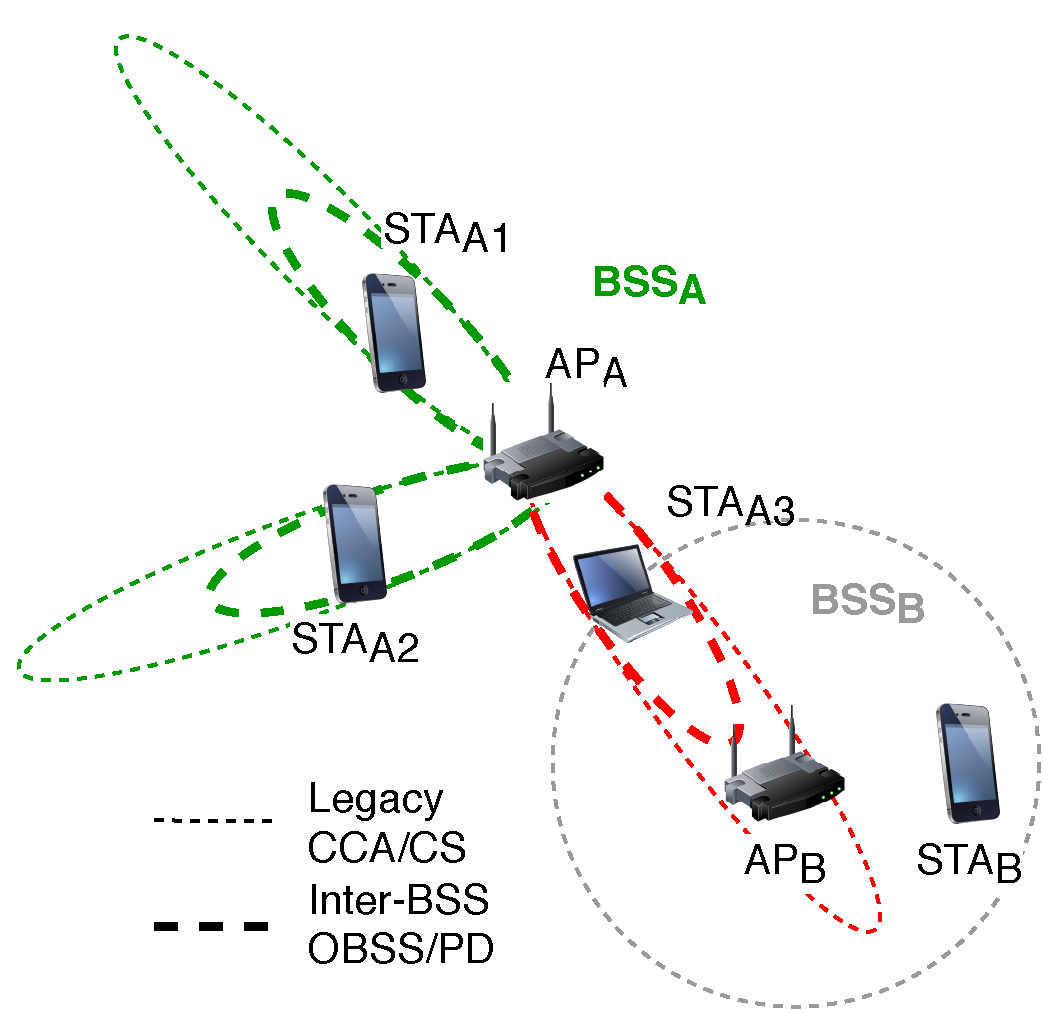
\includegraphics[width=0.4\columnwidth]{sr_and_beamforming}
	\caption{Potential application of SR combined with directional transmissions.}
	\label{fig:sr_and_beamforming}
\end{figure}

\begin{figure*}[ht!]
	\centering        
	\subfigure[Scenario]{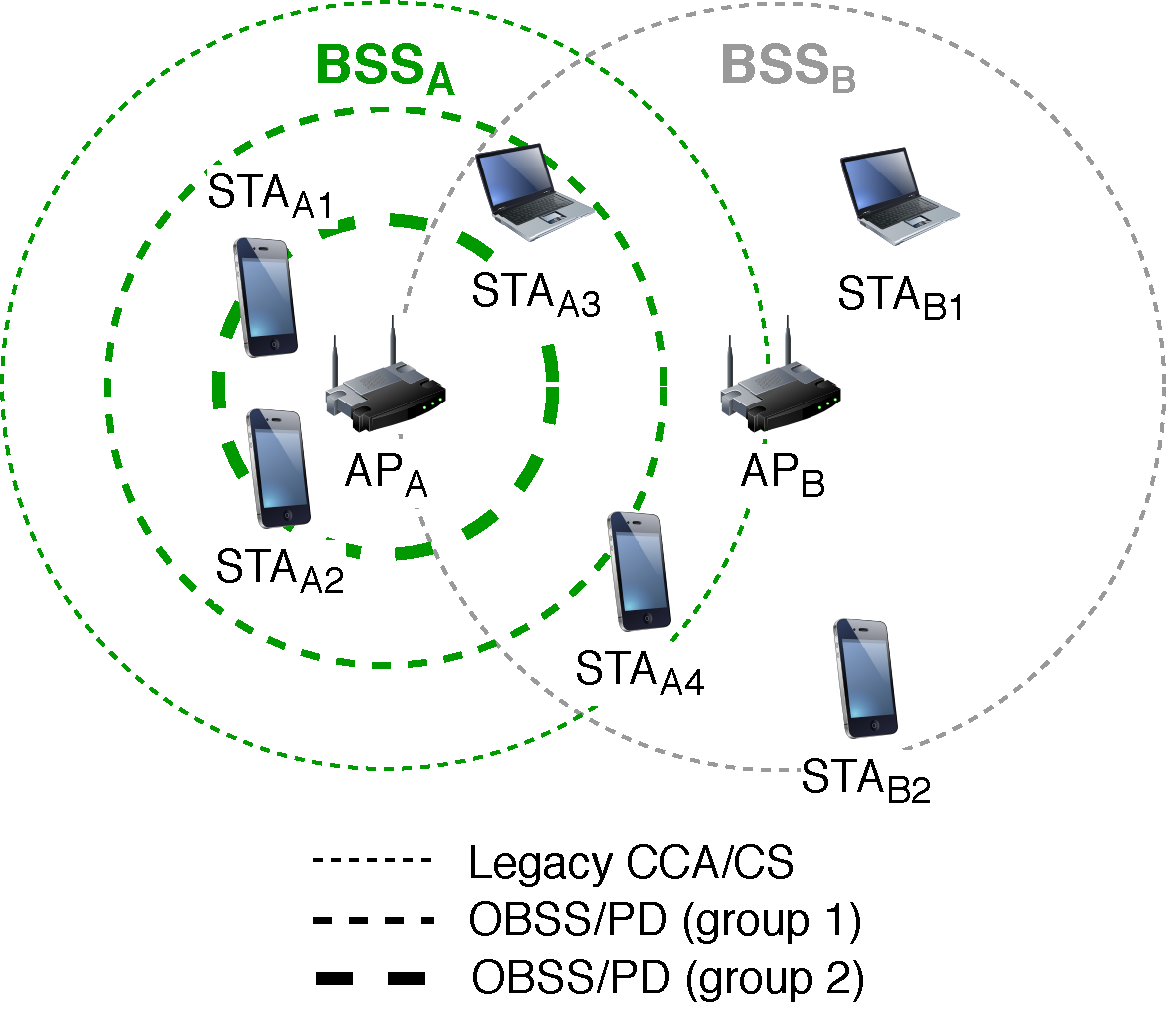
\includegraphics[width=0.4\columnwidth]{sr_and_tb}\label{fig:sr_and_tb_a}}
	\subfigure[Packets exchange]{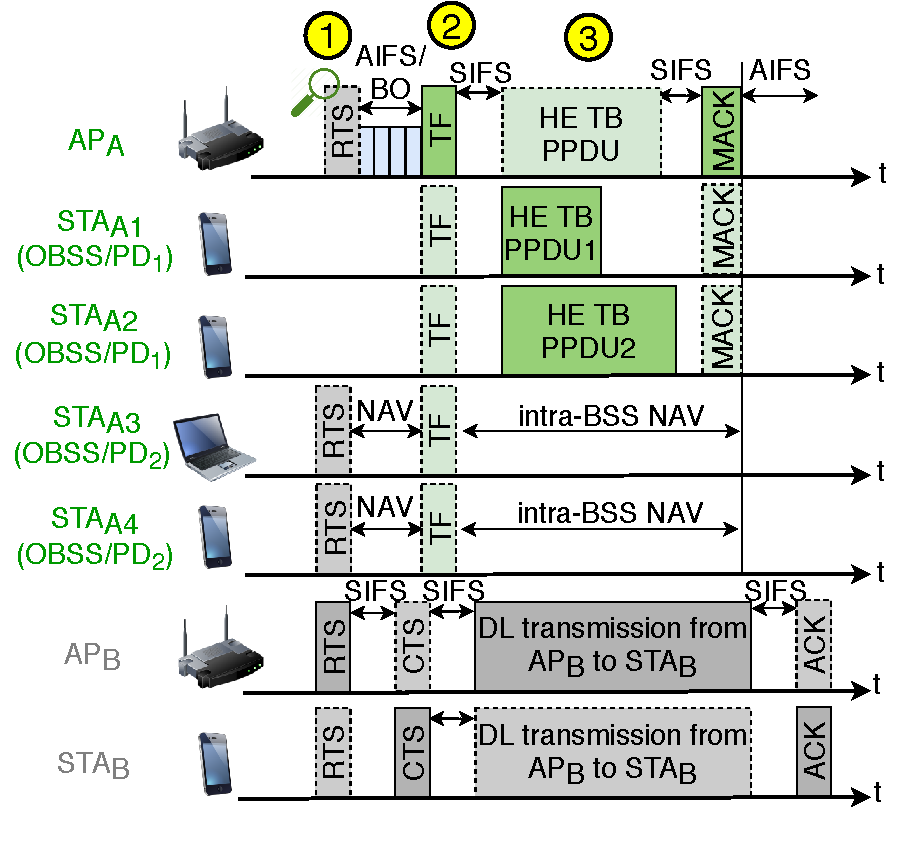
\includegraphics[width=.5\columnwidth]{sr_and_tb_b}\label{fig:sr_and_tb_b}}
	\caption{Potential application of SR combined with TB communications.}        
	\label{fig:sr_and_tb}
\end{figure*}

Similarly to the integration with directional antennas, the potential of SR can be further exploited through TB communications. In this case, users of a given BSS can be categorized into different types, so that different inter-BSS OBSS/PD values are assigned to them. Fig. \ref{fig:sr_and_tb_a} shows how users can be grouped based on different OBSS/PD thresholds. As a result, transmissions within the same BSS can be scheduled \textcolor{black}{differently}, thus improving spectral efficiency. In the proposed example, $\text{STA}_\text{A1}$ and $\text{STA}_\text{A2}$ belong to the first group because of their privileged position with respect to $\text{AP}_\text{A}$. Therefore, a more aggressive OBSS/PD threshold is employed when scheduling transmissions to these stations. The same reasoning can be applied to $\text{STA}_\text{A3}$, which, in this case, requires the usage of a more conservative OBSS/PD threshold for being scheduled in combination with SR. Finally, the legacy CCA/CS is used for $\text{STA}_\text{A4}$, in order to prevent negative interactions \textcolor{black}{concerning} $\text{BSS}_\text{B}$. It is worth pointing out that users belonging to different groups can be scheduled together, provided that the most restrictive OBSS/PD threshold is used. 

In Fig. \ref{fig:sr_and_tb_b}, we show a data transmission resulting from the combination of TB communications and SR. In the yellow point \#1, $\text{AP}_\text{A}$ detects an inter-BSS transmission from $\text{AP}_\text{B}$, which can be ignored by using the most aggressive OBSS/PD, i.e., the one devoted for STAs in group 1. Accordingly, it schedules an uplink transmission from $\text{STA}_\text{A1}$ and $\text{STA}_\text{A2}$ (yellow point \#2). Finally, $\text{AP}_\text{A}$ receives the scheduled transmissions from group 1 (yellow point \#3).

\subsection{Artificial Intelligence to Address Spatial Reuse Optimization}
In light of the challenges posed by the 11ax SR operation, Artificial Intelligence (AI) emerges as a potential solution. In particular, WLANs are characterized by being highly varying in terms of users and channel dynamics. Moreover, we typically find decentralized deployments, at which none or little coordination is allowed. Hence, online learning stands as a suitable technique to address the optimization of SR in WLANs. In fact, many works on OBSS/PD adjustment, such as DSC \cite{smith2015dynamic} and COST \cite{selinis2018control}, are based on iterative methods. 

\textcolor{black}{Machine Learning (ML), and more precisely, Reinforcement Learning (RL), can improve the existing methods' performance. RL has been shown to fit with the decentralized nature of IEEE 802.11 WLANs \cite{long2007non, naddafzadeh2010distributed, zhou2011reinforcement, ghadimi2017reinforcement, wilhelmi2019collaborative, wilhelmi2019potential}. In particular, the usage of RL allows capturing subtle information that cannot be predicted before-hand (for instance, regarding inter-BSS interactions). Such information enables conducting a learning-based procedure, which is aimed at increasing performance while reducing the number of undesired situations (e.g., poor fairness).}

% ----------------------------------
% -
% 	-- Conclusions --
% -
% ----------------------------------
\section{Conclusions}
\label{section:conclusions}
In this paper, we have provided an extensive tutorial of the IEEE 802.11ax SR operation, which aims to maximize the performance of next-generation WLANs by increasing the number of parallel transmissions. Our purpose has been to do so in a clear and easy-to-understand manner. Thus, significant efforts have been made in providing meaningful examples of the different specifications related to SR. %First of all, we have presented the concepts that enable such an operation, which mostly refer to BSS coloring, SRGs, and scheduled transmissions. From there, we described the 11ax SR specification, which has been supported with illustrative examples. 

Apart from the tutorial, we have modeled the SR operation analytically using CTMNs. Through this model, we have analyzed the new kind of inter-BSS interactions that may result from applying SR in an OBSS. In particular, we have considered BSSs with a single STA, but more complex interactions are expected to happen when applying the SR operation in BSSs with multiple STAs. Apart from the analytical analysis, we have implemented the 11ax SR operation in the Komondor simulator. The potential of SR in large-scale scenarios has been evaluated through extensive simulations. \textcolor{black}{These results open the door to new contributions concerning the evaluation of the 11ax SR operation in more sophisticated environments, including nodes mobility, complex uplink/downlink traffic models, or heterogeneous deployments.}	

\textcolor{black}{Besides the} significant improvements achieved by the SR operation, other important aspects have been identified. First of all, it is important to highlight the non-intrusive characteristic of the SR operation. In particular, devices using SR can increase their performance without affecting other overlapping networks or preventing them \textcolor{black}{from transmitting}. This is a key feature to sustain performance growth. Moreover, the SR operation has been shown to perform better in scenarios with a high level of interference, i.e., high-density scenarios with a high traffic load. This confirms the utility of the SR for dense next-generation wireless networks.

However, finding the best SR configuration is far from trivial (it is a combinatorial problem), and remains an open problem. Indeed, the 11ax amendment does not provide \textcolor{black}{any specifications and guidelines} on this matter. We left as future work the design of mechanisms able to find the optimal parameters within the IEEE 802.11ax SR operation. For that purpose, the usage of RL can be particularly targeted. \textcolor{black}{Besides}, SR can evolve and be combined with other novel techniques such as directional transmissions or distributed OFDMA \textcolor{black}{to achieve further performance gains.}

\appendices
\section{IEEE 802.11ax Frames}
\label{section:frames}
In this Section, we introduce the type of frames that are considered in the 11ax amendment. Such information is key \textcolor{black}{to understand the SR operation better.}

% HE PPDUs
\subsection{HE PPDU formats}
Below, we briefly describe the Physical Protocol Data Unit (PPDU) formats available in the 11ax:
\begin{itemize}
	\item SU (Single User) HE PPDU: are meant for single user communications.
	\item  HE Extended Range HE PPDU: are meant for single user long-range transmissions, hence only contemplate 20 MHz bandwidths in a single spatial stream.
	\item  MU (Multi-User) HE PPDU: due to the OFDMA operation, such kind of PPDUs are meant for multiple transmissions to one or more users.
	\item Trigger-Based (TB) HE PPDU: in this case, MU UL transmissions are scheduled by the AP, which decides which STAs are expected to transmit during a specific elapse of time. The TB HE PPDUs can make use of OFDMA and/or MU-MIMO.
\end{itemize}

The new fields included in the abovementioned HE PPDU formats are HE Signal A Field (HE-SIG-A), HE Signal B Field (HE-SIG-B), HE Short Training Field (HE-STF), and HE Long Training Field (HE-LTF), which are shown in Fig. \ref{fig:appendix_1}.
\begin{figure}[ht!]
	\centering
	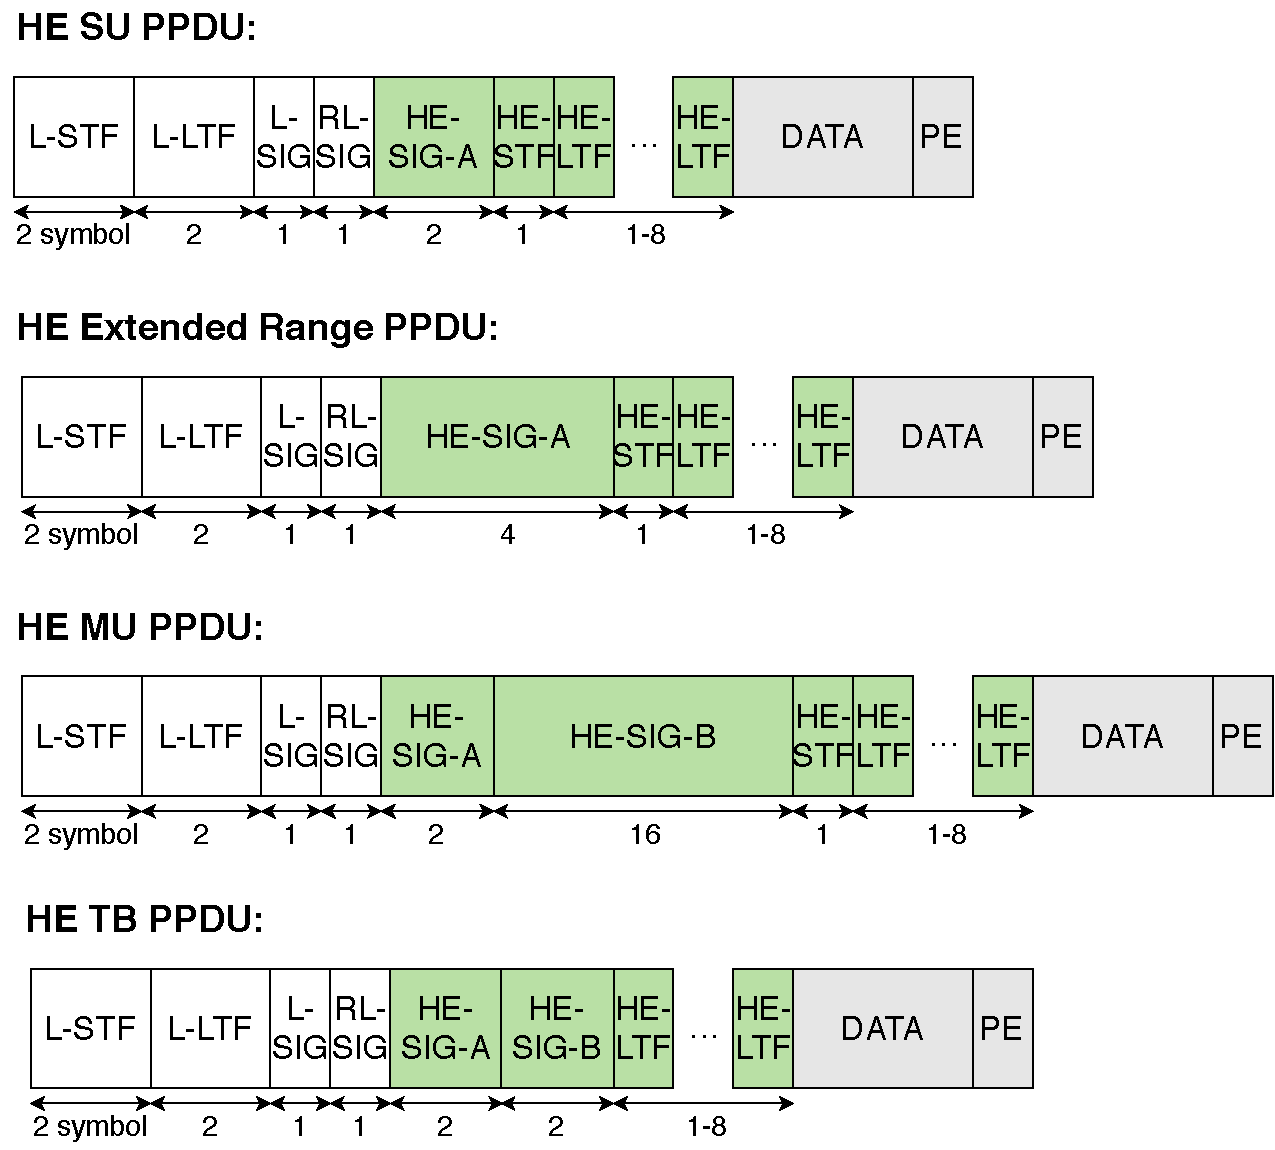
\epsfig{file=fig_25.pdf, width=.55\columnwidth}
	\caption{HE PPDU formats. New IEEE 802.11ax fields are highlighted in green.}
	\label{fig:appendix_1}
\end{figure}

Among the new fields, we highlight HE-SIG-A, which includes the following elements related to the SR operation:
\begin{itemize}
	\item BSS color: it is used as an identifier of the BSS (refer to Section \ref{section:bss_coloring}).
	\item Spatial Reuse: this field indicates whether the HE node supports the SR operation. If this is the case, the field also indicates the limit on the transmission power to be used during the SR opportunities that can potentially be detected. Notice that a single Spatial Reuse field (of length of 4 bits) is carried in HE SU/MU/ER PPDUs,  while HE TB PPDUs may include up to four Spatial Reuse fields. In particular, each field is meant for the SR operation in each allowed channel width (i.e., 20 MHz, 40 MHz, 80 MHz, and 160 MHz).
\end{itemize}

Besides supporting HE PPDU formats, HE STAs are required to be compatible with legacy formats. More information regarding HE PPDU formats can be found in \cite{rhode2017whitepaper}. 

% Other
\subsection{Management Fields for Spatial Reuse}
Some operations auxiliary to SR are enabled by control frames, which are Beacon, Probe Response, and (Re)Association Response frames. Beacons are used by APs to announce the presence of a BSS and to provide details of it. \textcolor{black}{In particular, by means of Beacons, an AP may request an STA to gather information regarding the environment:} information of BSSs matching a particular BSSID and/or SSID, channel-specific report, or HE Operation element of neighboring HE APs. With this information, the AP can make decisions related to the SR operation. Regarding Probe Responses, they are meant to carry the information requested by devices scanning the area through Probe Requests. Finally, (Re)Association Response frames are sent by APs to which a STA attempts to associate.

The abovementioned kind of frames are important to the SR operation because they carry, among other fields, the following information:
\begin{itemize}
	\item \textbf{HE Capabilities:} it is used by HE STAs to announce support for certain HE capabilities.
	\item \textbf{HE Operation:} it defines the operation of HE STAs. For instance, it indicates whether BSS coloring is enabled or not.
	\item \textbf{BSS Color Change Announcement:} it is used by HE APs to indicate the utilization of a new BSS color so that the associated STAs and the surrounding devices can be aware of the change.
	\item \textbf{Spatial Reuse Parameter Set (SRPS) element:} this element provides the necessary information to carry out the OBSS/PD-based SR operation, which is defined in Section \ref{section:obss_pd_based}. The SRPS element is further defined in Appendix \ref{section:srps}.
\end{itemize}

\subsubsection{Spatial Reuse Parameter Set element}
\label{section:srps}
The format of the SRPS element is optionally present in Beacons, Probe Responses and (Re)Association responses. Fig. \ref{fig:appendix_2} shows the SRPS element in detail.
% SR PARAMETER SET ELEMENT
\begin{figure}[ht!]
	\centering
	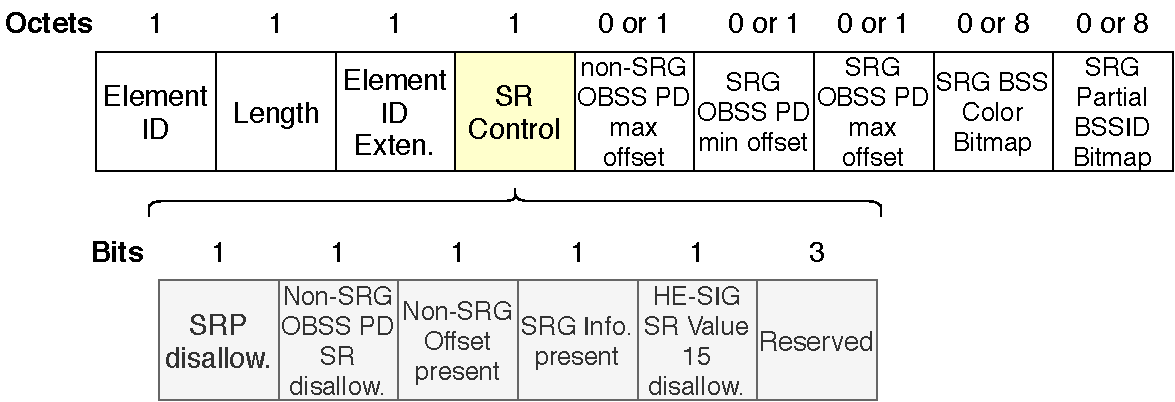
\epsfig{file=fig_26.pdf, width=.7\columnwidth}
	\caption{Spatial Reuse Parameter Set element.}
	\label{fig:appendix_2}
\end{figure}

Each item in the SRPS element is next described:
\begin{itemize}
	\item Element ID: set to 255.
	\item Length: not defined.
	\item Element ID extension: set to 39.
	\item SR Control field: contains the following parameters:
	\begin{itemize}
		\item PSR Disallowed: indicates whether PSR transmissions are allowed or not at non-AP STAs associated with the AP that transmitted this element.
		\item Non-SRG OBSS/PD SR Disallowed: indicates whether non-SRG OBSS/PD SR transmissions are allowed or not at non-AP STAs associated with the AP that transmitted this element.
		\item Non-SRG Offset Present: indicates whether the Non-SRG OBSS/PD Max Offset subfield is present in the element.
		\item SRG Information Present: indicates whether the SRG OBSS/PD Min Offset, SRG OBSS/PD Max Offset, SRG BSS Color Bitmap, and SRG Partial BSSID Bitmap subfields are present in the element.
		\item HE-SIG-A Spatial Reuse Value 15 disallow: indicates whether non-AP STAs associated with the AP that transmitted this element may set the TXVECTOR parameter SPATIAL\_REUSE to PSR\_AND\_NON-SRG-OBSS-PD\_PROHIBITED to avoid PSR transmissions.
	\end{itemize}
	\item Non-SRG OBSS/PD Max Offset: integer to generate the maximum Non-SRG OBSS/PD threshold.
	\item Non-SRG OBSS/PD Min Offset: integer to generate the minimum Non-SRG OBSS/PD threshold.
	\item SRG OBSS/PD Max Offset: integer to generate the maximum SRG OBSS/PD threshold.
	\item SRG BSS Color Bitmap: indicates which BSS Color values are used by the members of the SRG.
	\item SRG Partial BSSID Bitmap: indicates which partial BSSID values are used by members of the SRG.
\end{itemize}

\section*{Acknowledgment}

This  work  has  been  partially  supported  by  the  Spanish Ministry of Economy and Competitiveness under the Maria de Maeztu  Units  of  Excellence  Programme  (MDM-2015-0502), by PGC2018-099959-B-100 (MCIU/AEI/FEDER,UE), by the Catalan Government under SGR grant for research support (2017-SGR-11888), by SPOTS project (RTI2018-095438-A-I00) funded by the Spanish Ministry of Science, Innovation and Universities, and  by a Gift from the Cisco University Research Program (CG\#890107, Towards Deterministic Channel Access in High-Density WLANs) Fund, a corporate advised fund of Silicon Valley Community Foundation.
The authors would like to thank Malcolm Smith and Adrian Garcia for their thorough reviews and insightful comments.
	
%%%%%%%%%%%%%%%%%%%%%%%%%
%%%  BIBLIOGRAPHY    
%%%%%%%%%%%%%%%%%%%%%%%%%

\bibliographystyle{unsrt}
\bibliography{references}

\end{document}